\begin{figure*}
	\centering
	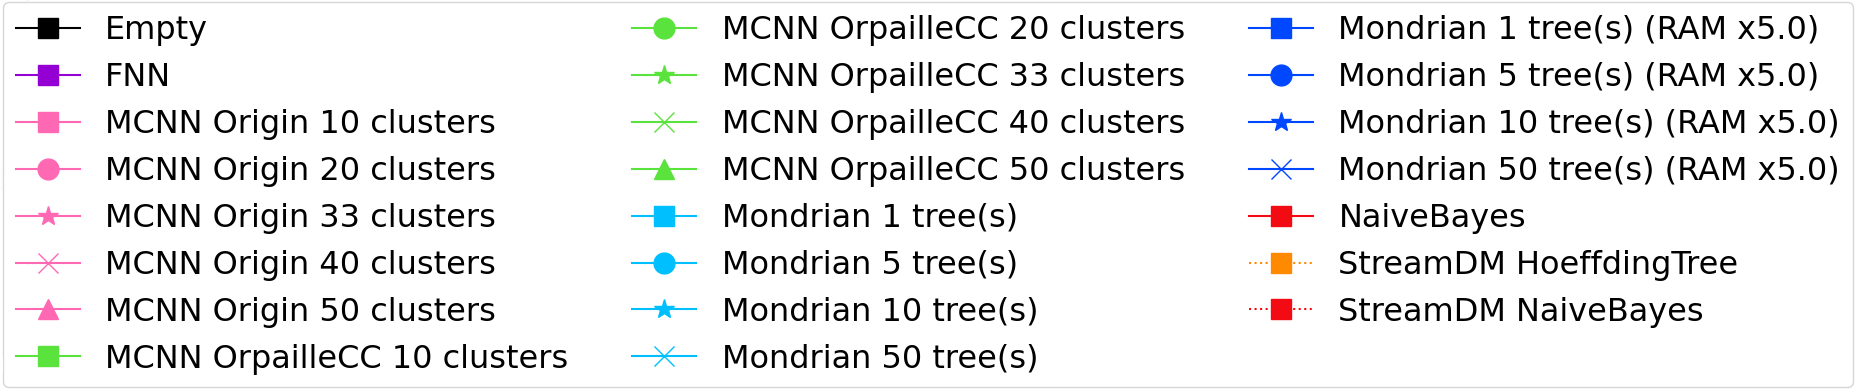
\includegraphics[width=0.8\linewidth]{figures/legend.png}
	\begin{subfigure}[t]{.49\linewidth}
		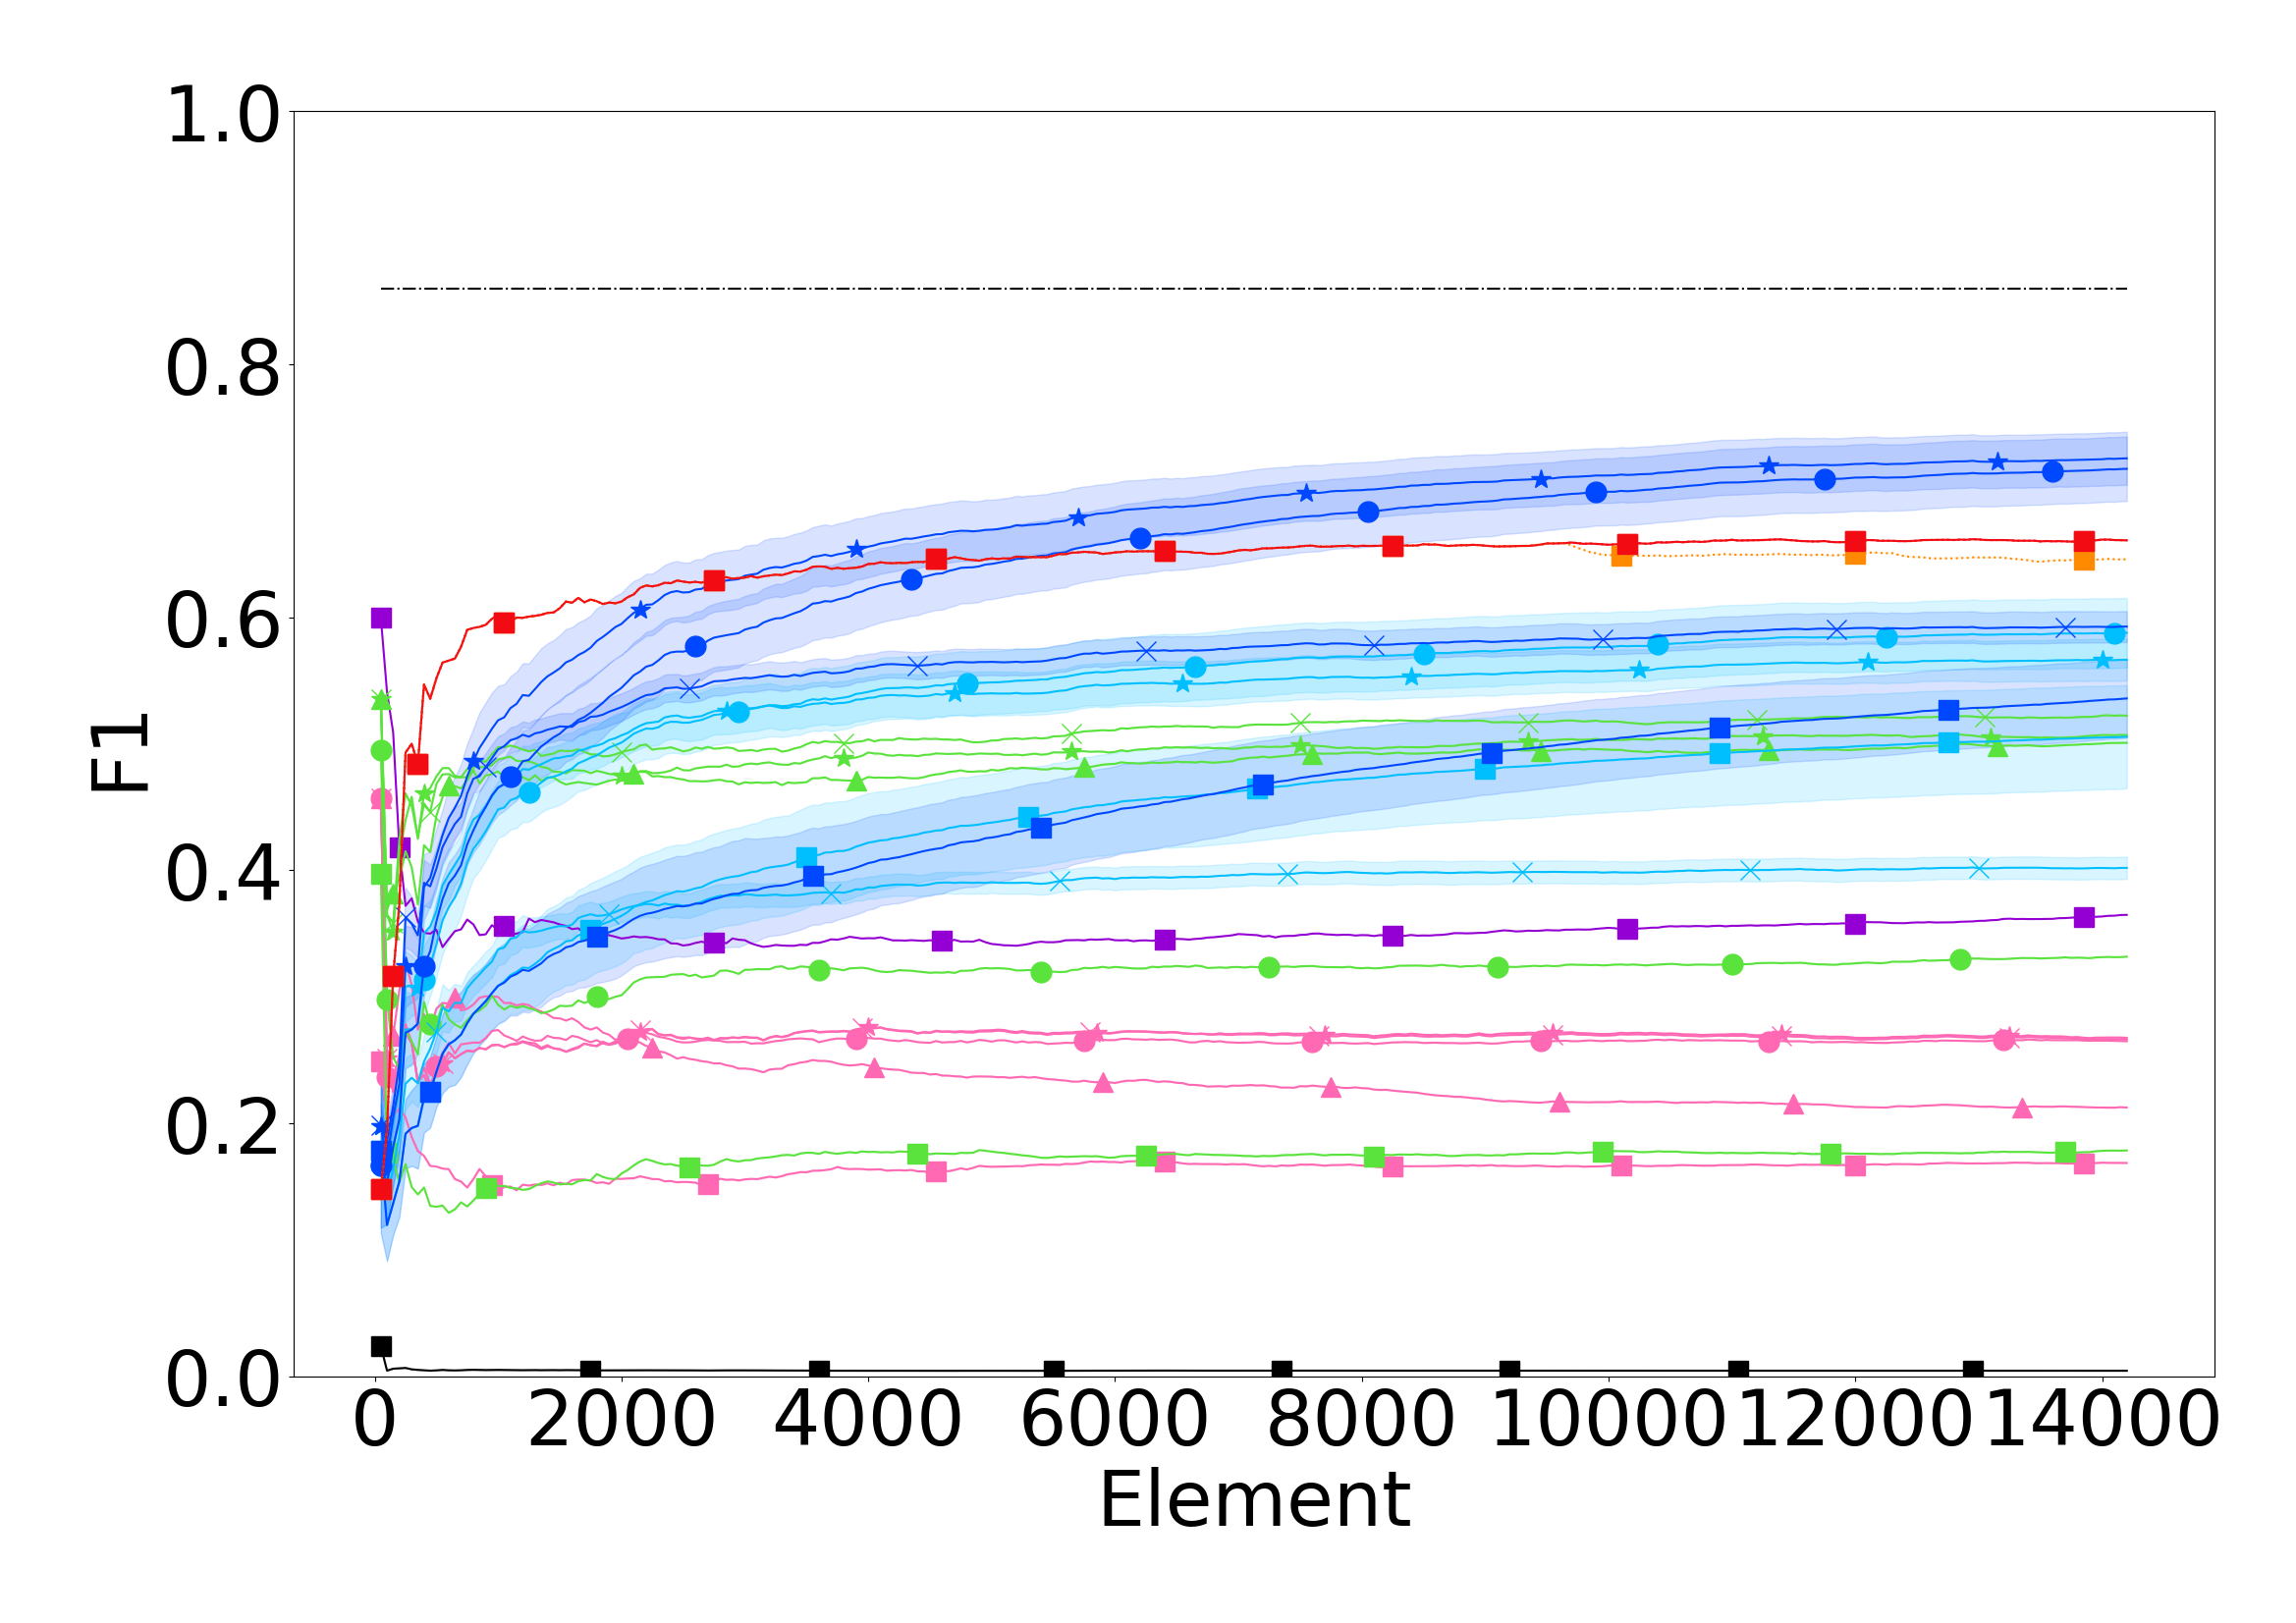
\includegraphics[width=\linewidth]{figures/results/banos_6_f1_std.png}
		\caption{\banosdataset}
		\label{fig:f1-banos}
	\end{subfigure}
	\begin{subfigure}[t]{.49\linewidth}
		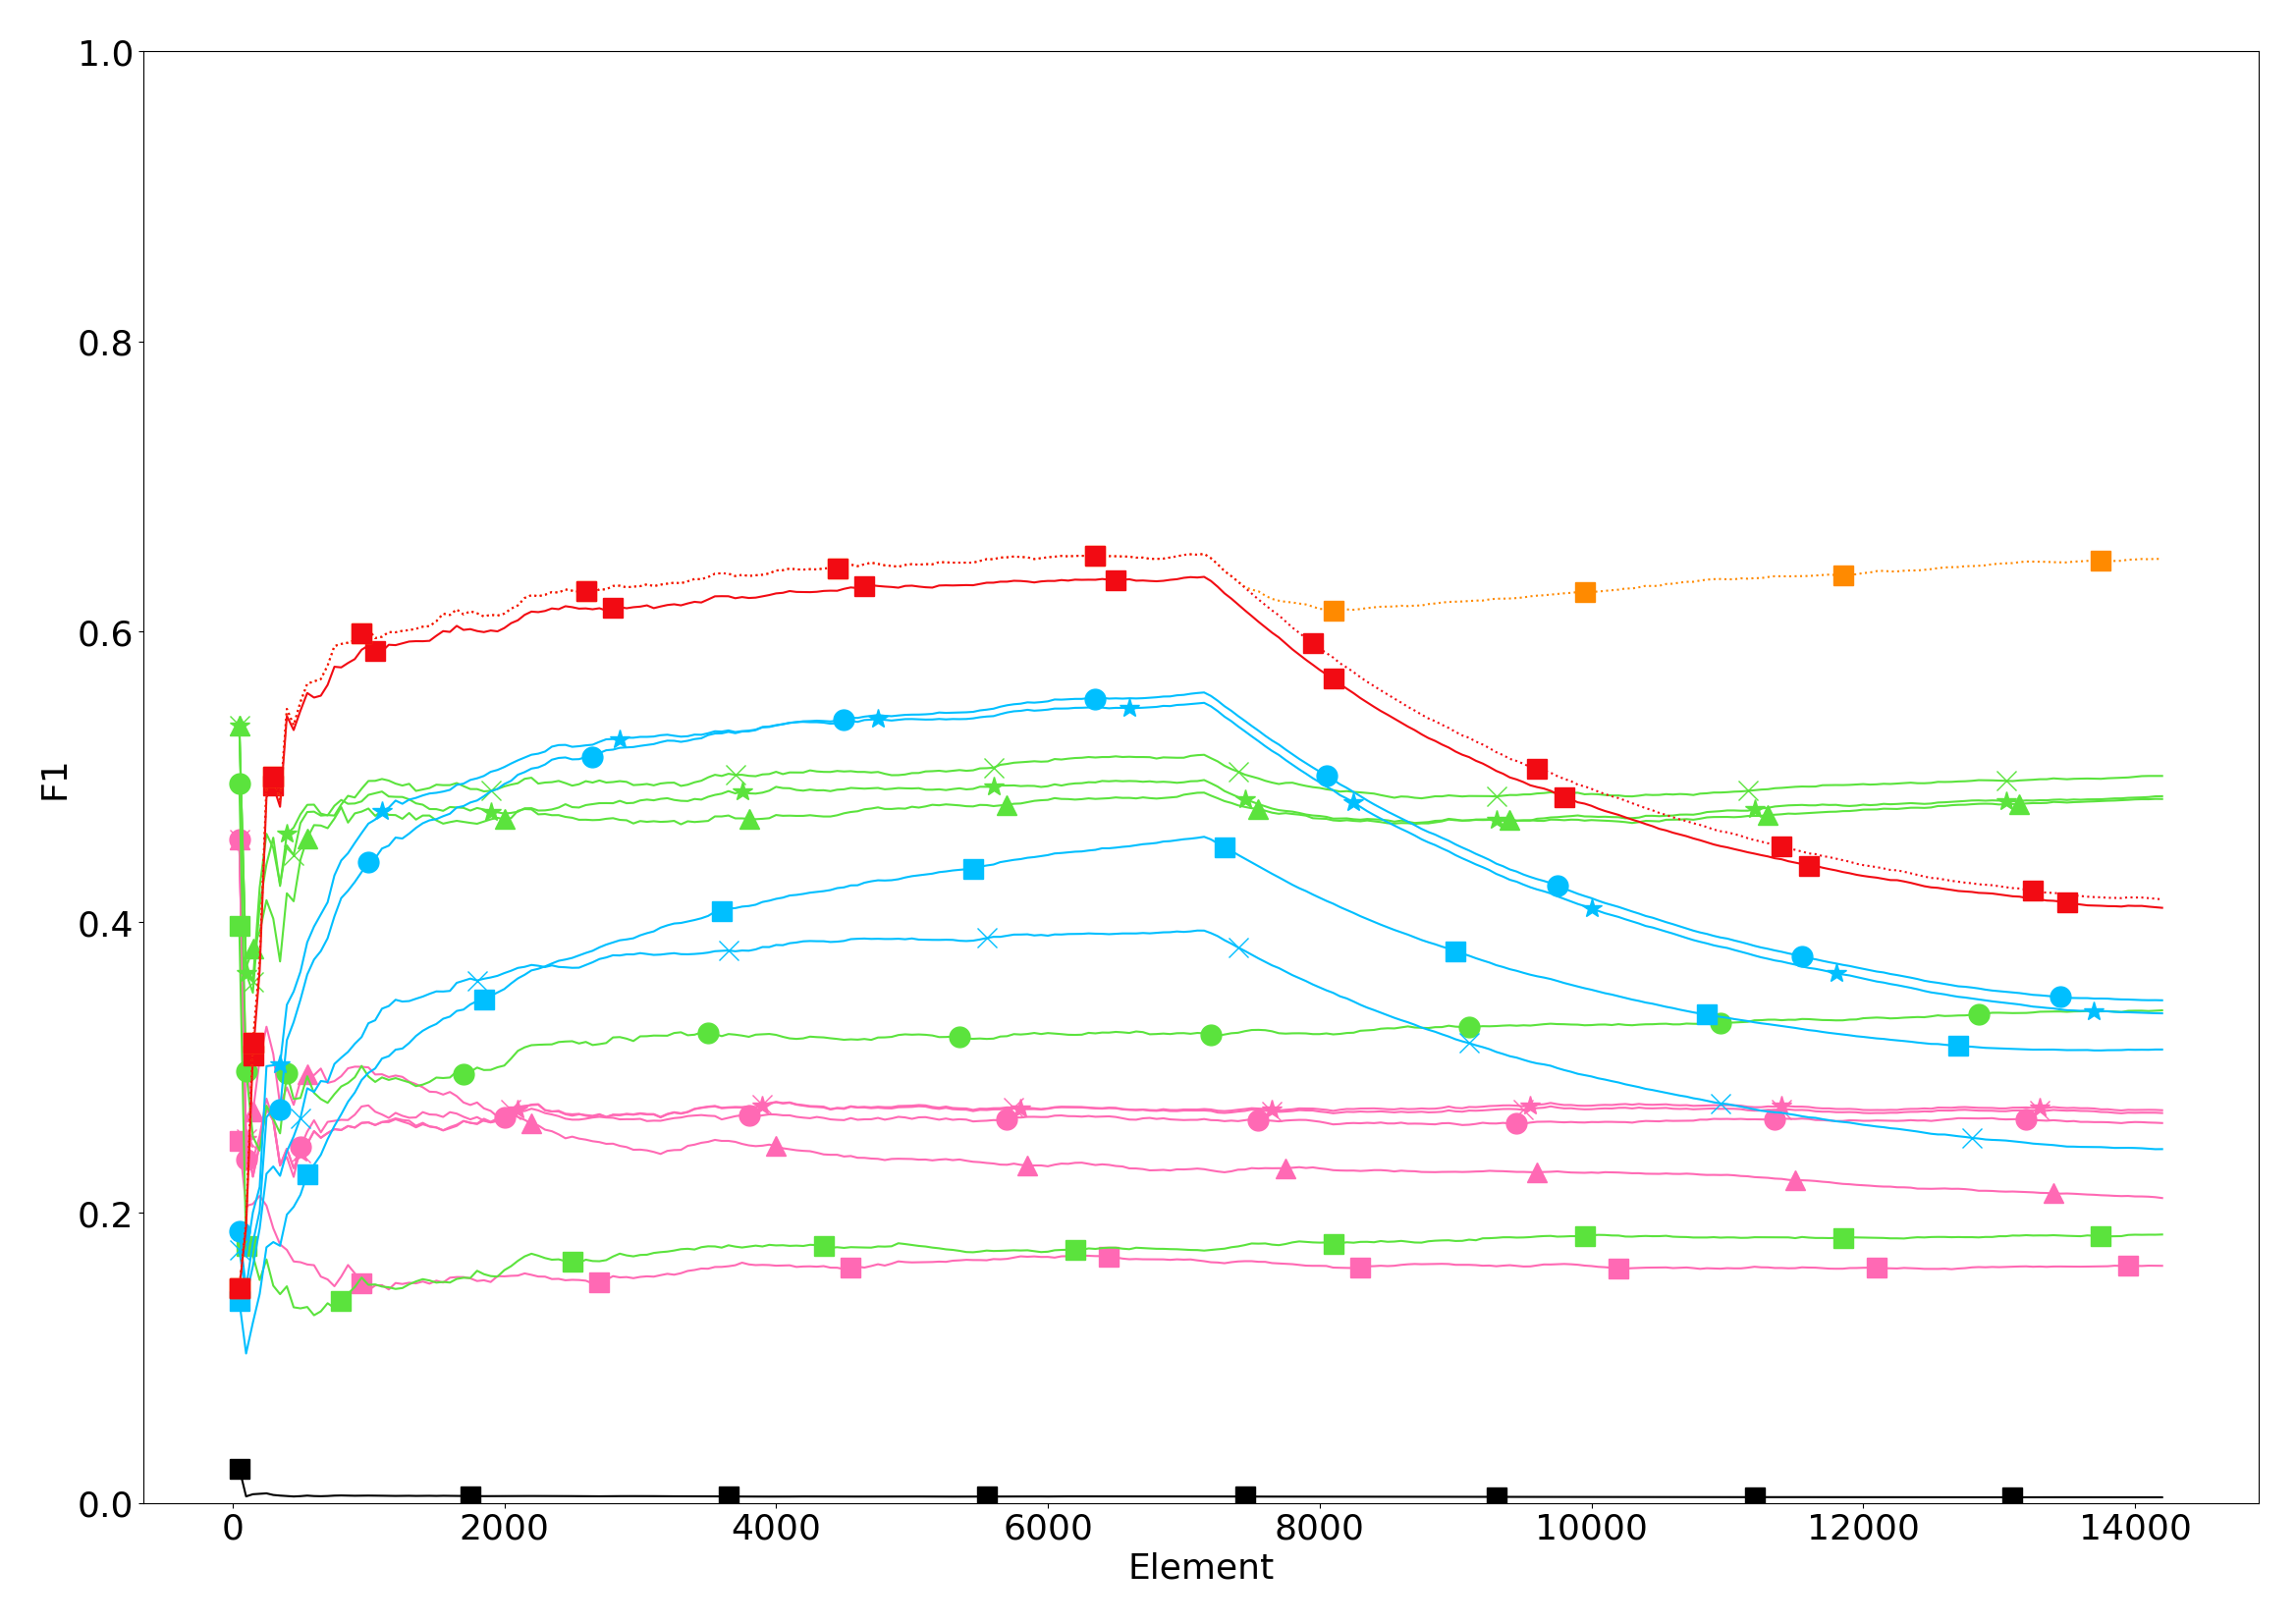
\includegraphics[width=\linewidth]{figures/results/drift_6_f1.png}
		\caption{\banosdataset (with Drift)}
		\label{fig:f1-drift}
	\end{subfigure}\\
	\begin{subfigure}[t]{.49\linewidth}
		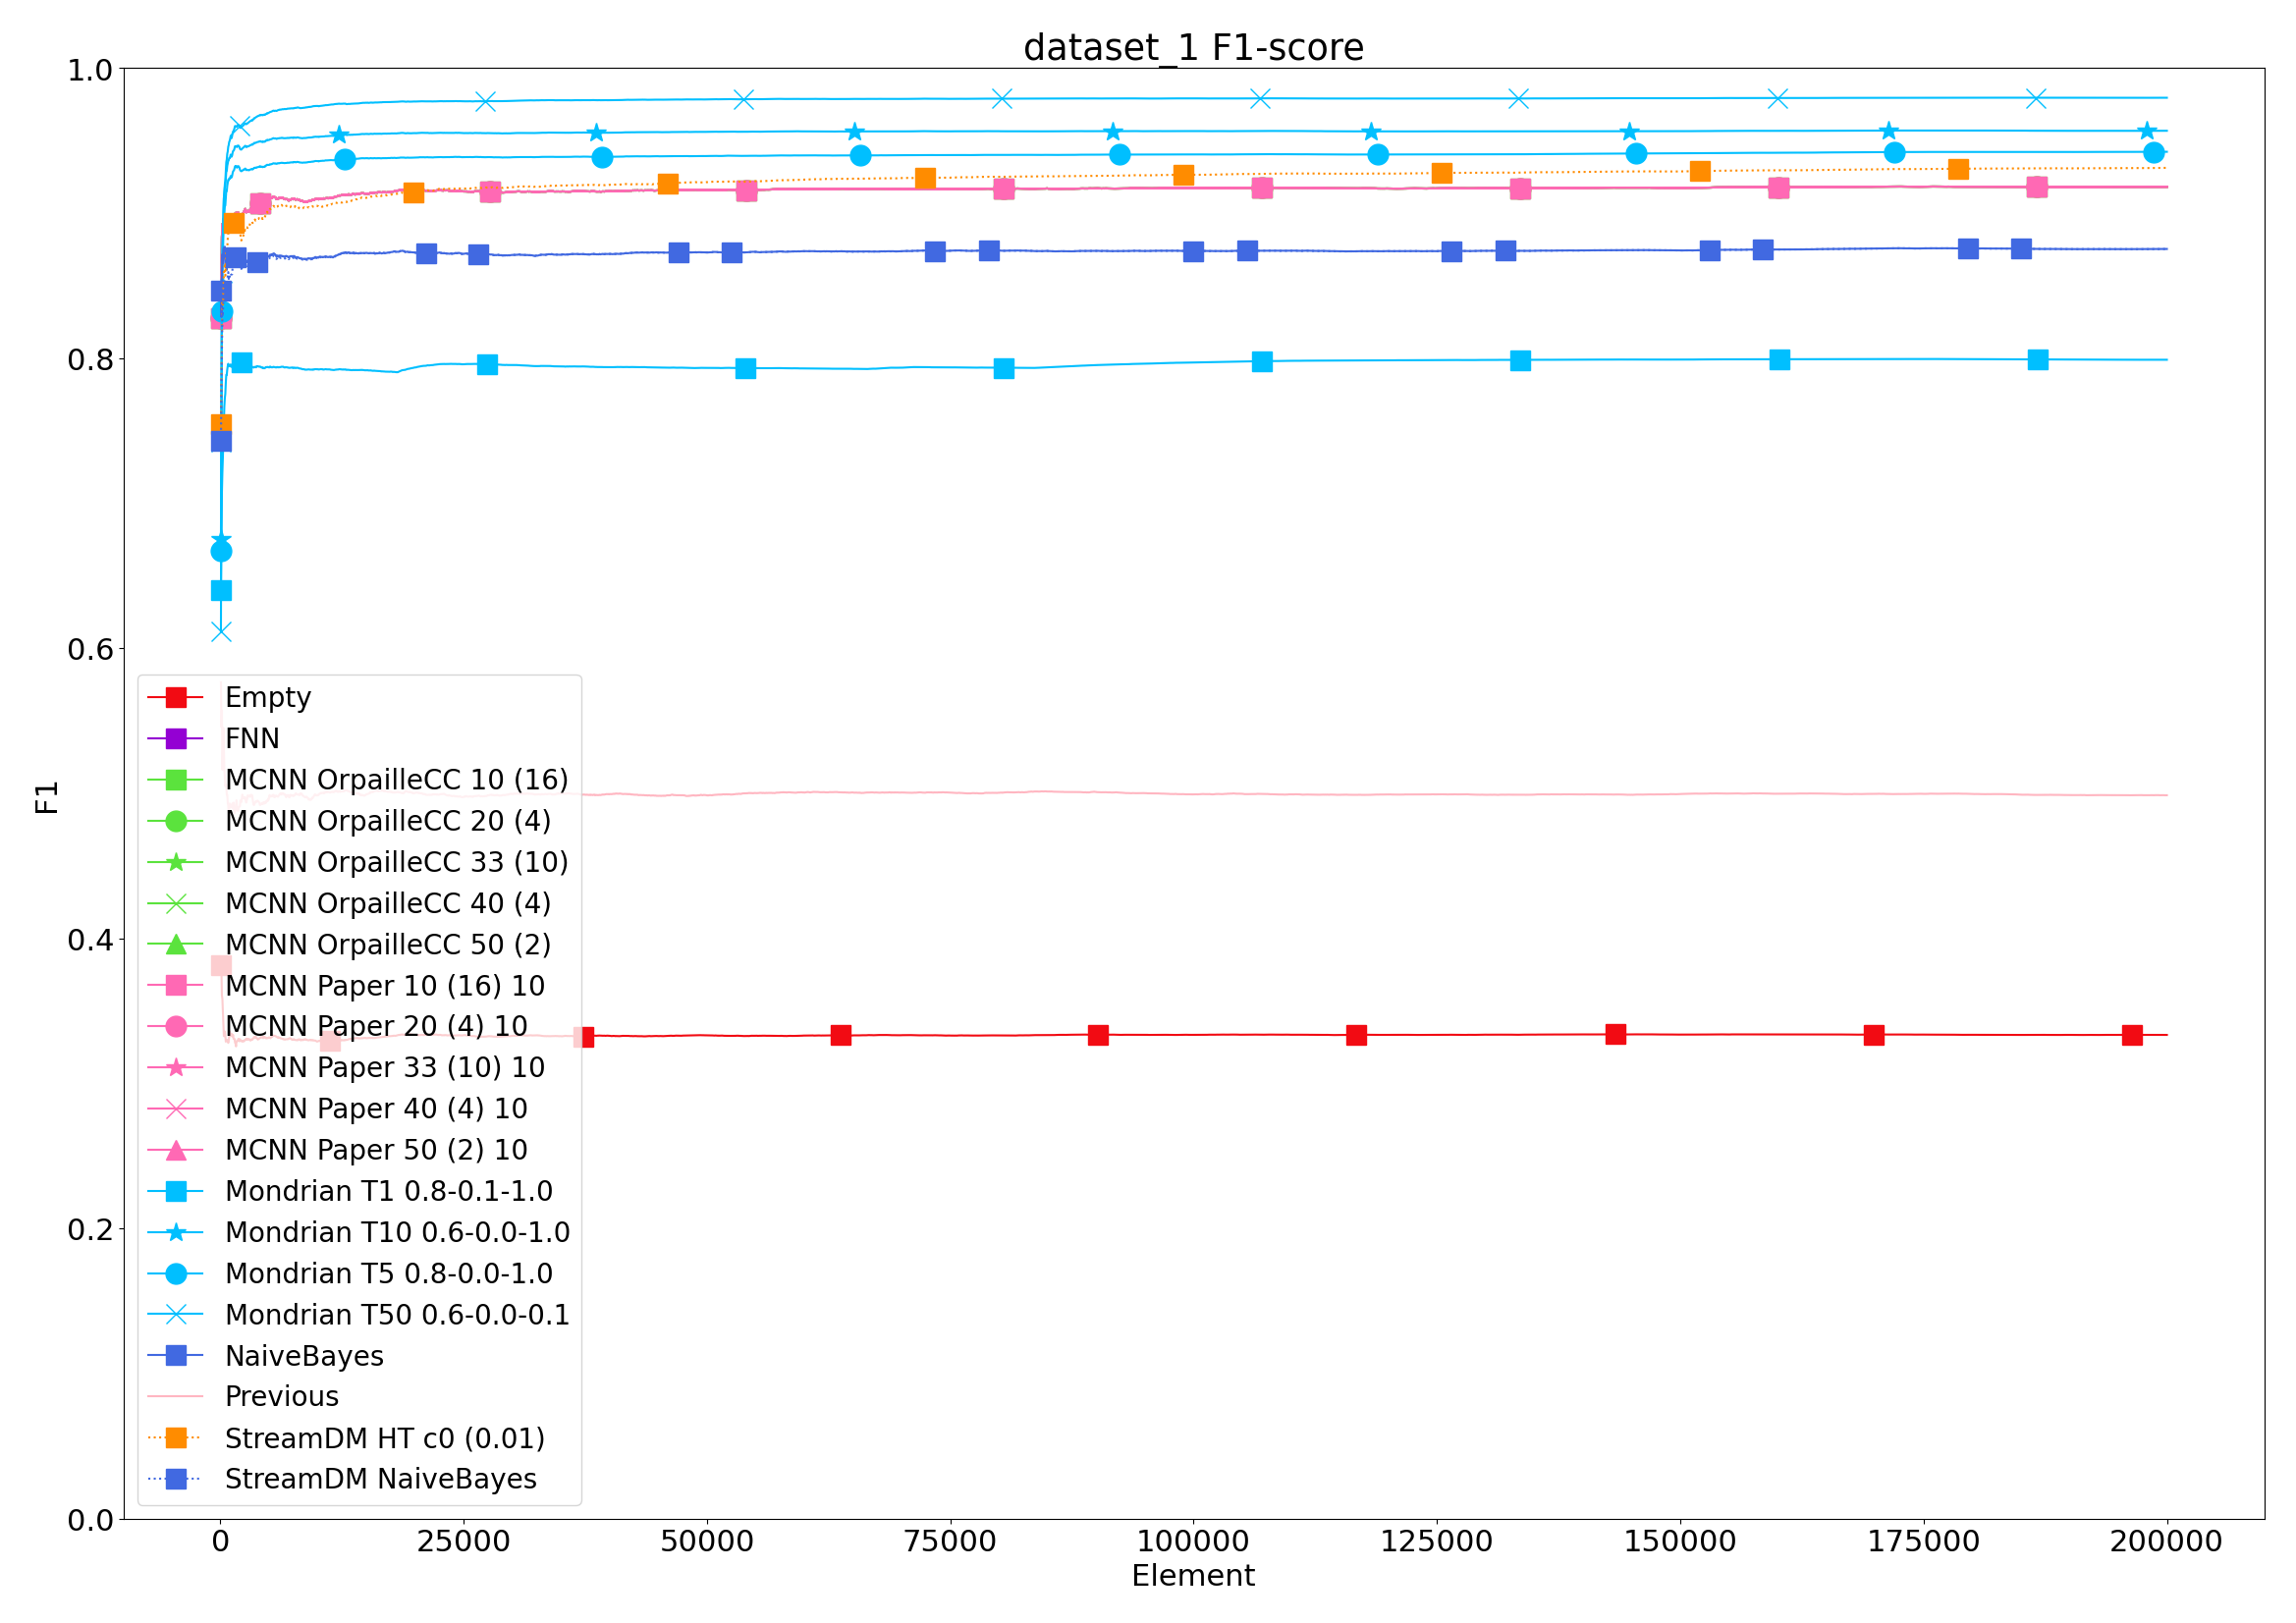
\includegraphics[width=\linewidth]{figures/results/dataset_1_f1.png}
		\caption{Hyperplane (MOA)}
		\label{fig:f1-dataset_1}
	\end{subfigure}
	\begin{subfigure}[t]{.49\linewidth}
		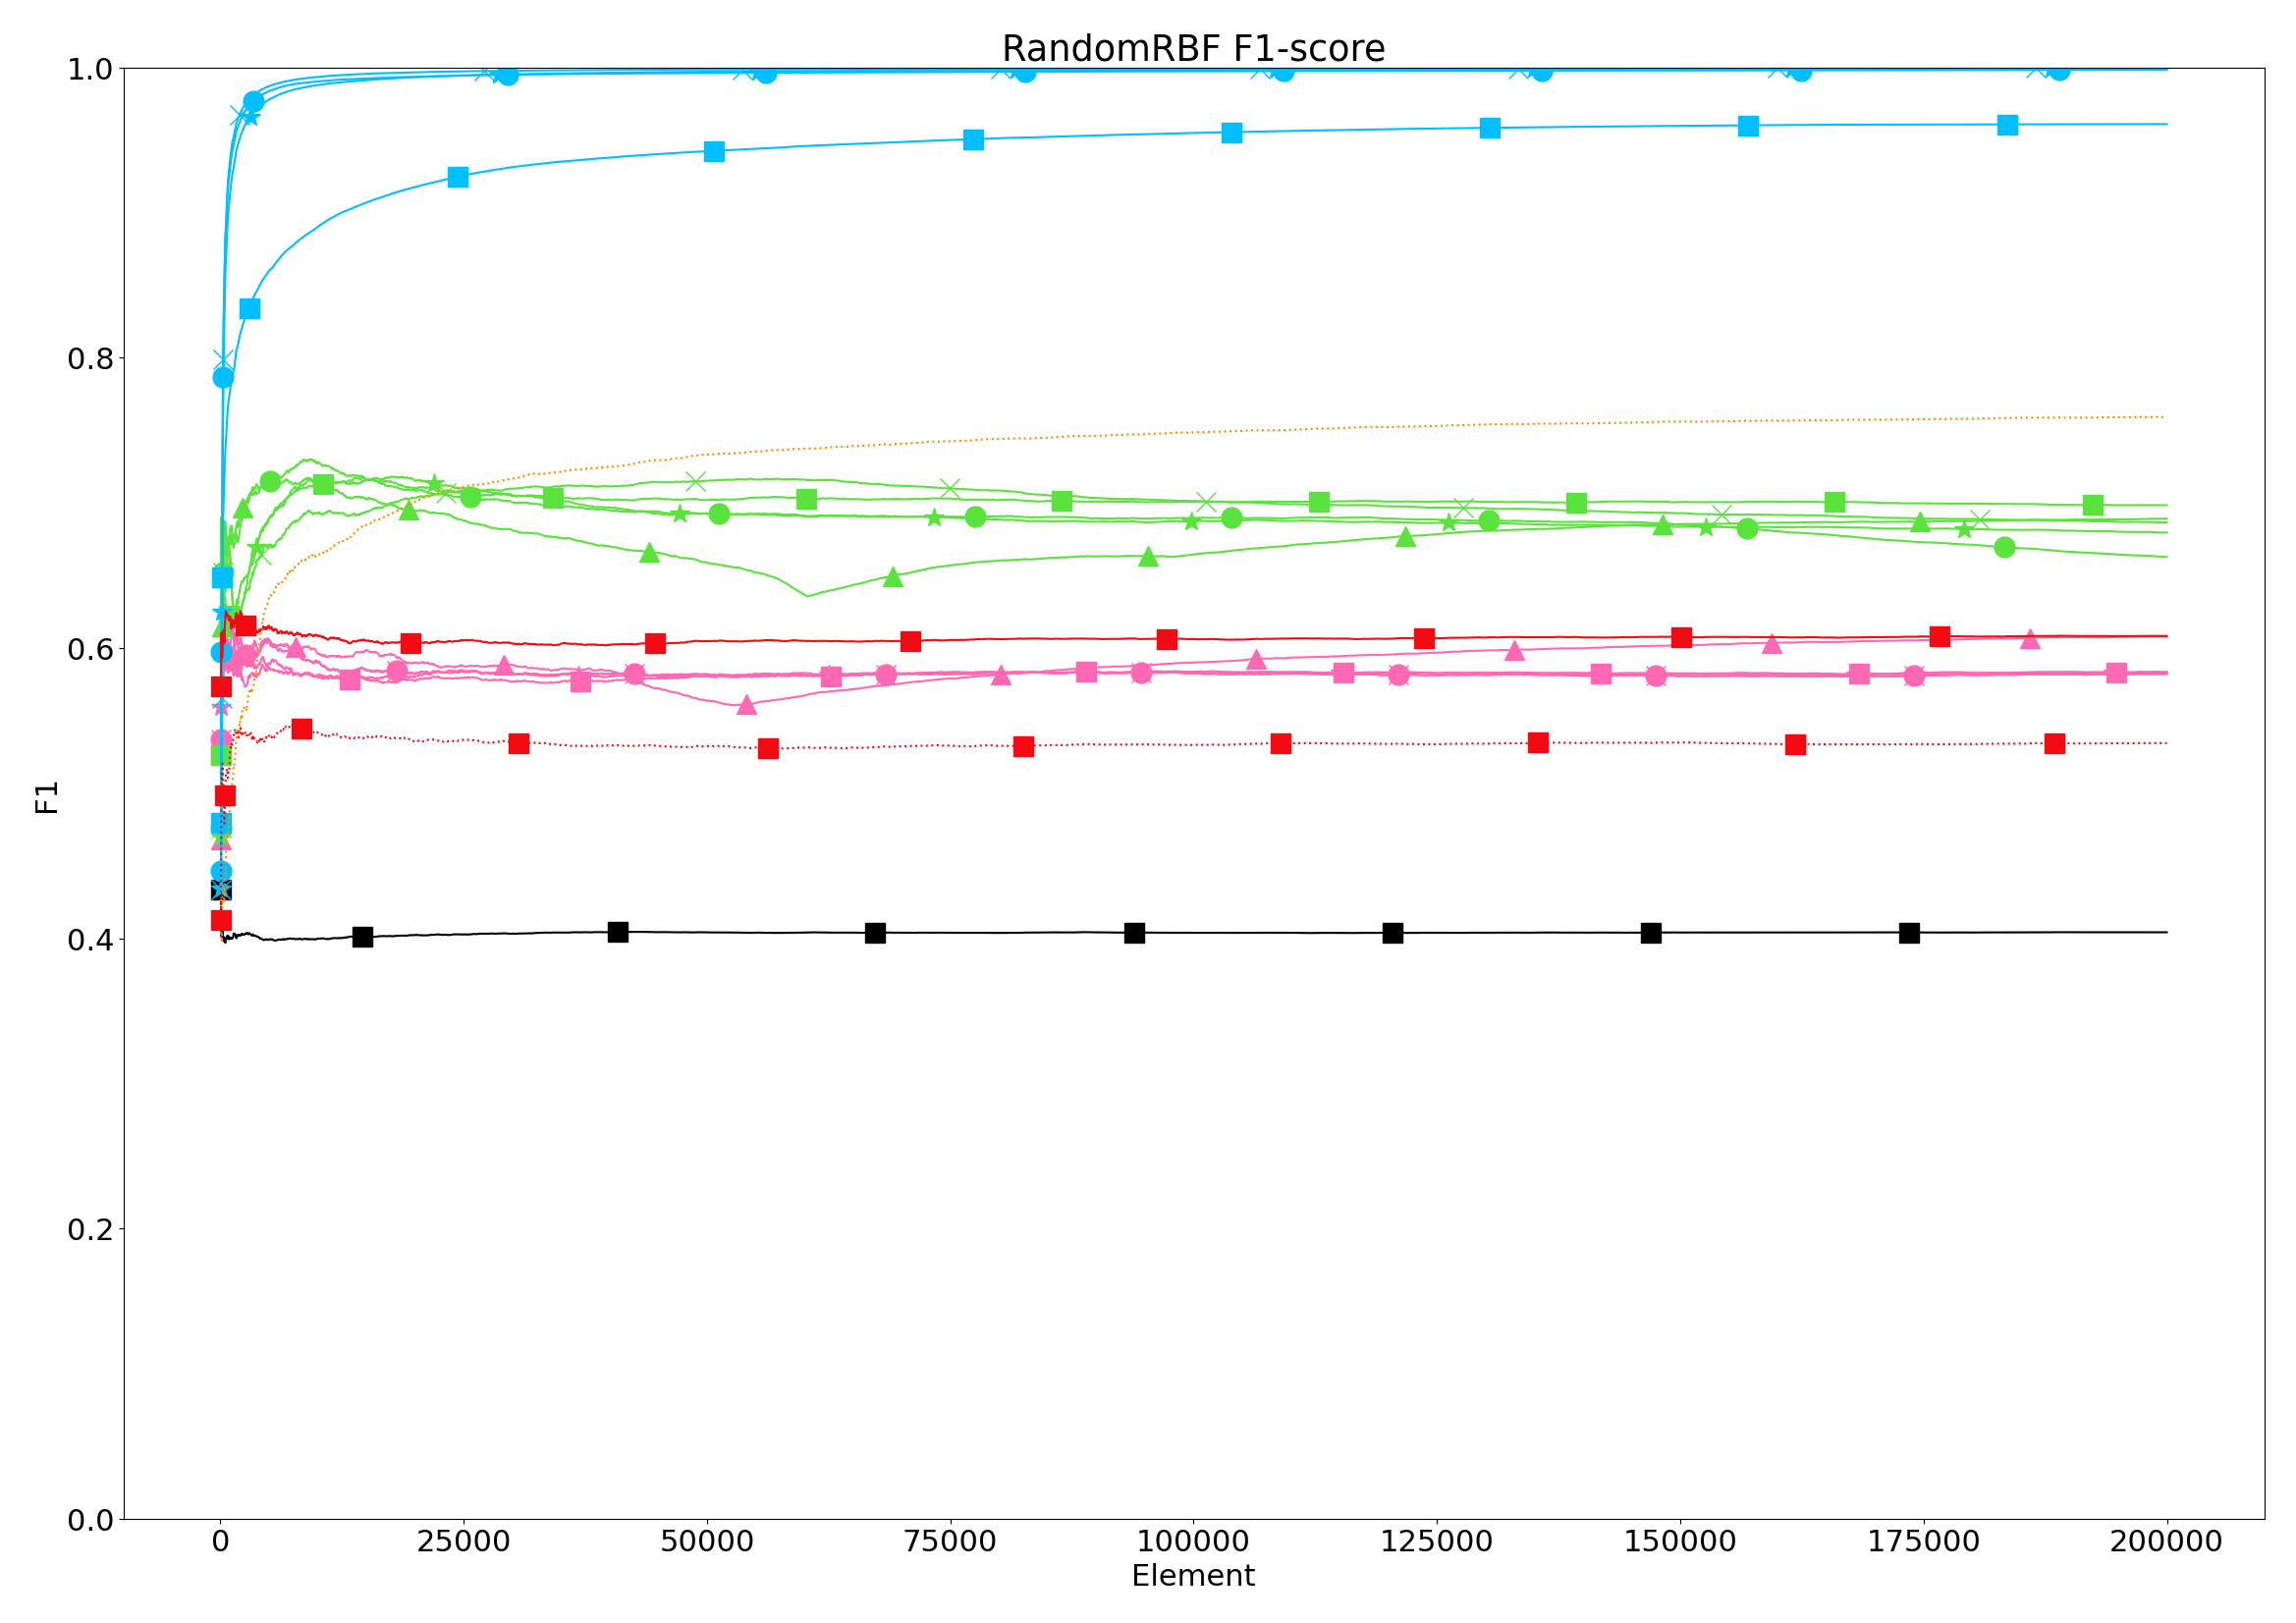
\includegraphics[width=\linewidth]{figures/results/dataset_2_f1.png}
		\caption{RandomRBF (MOA)}
		\label{fig:f1-dataset_2}
	\end{subfigure}\\
	\begin{subfigure}[t]{.49\linewidth}
		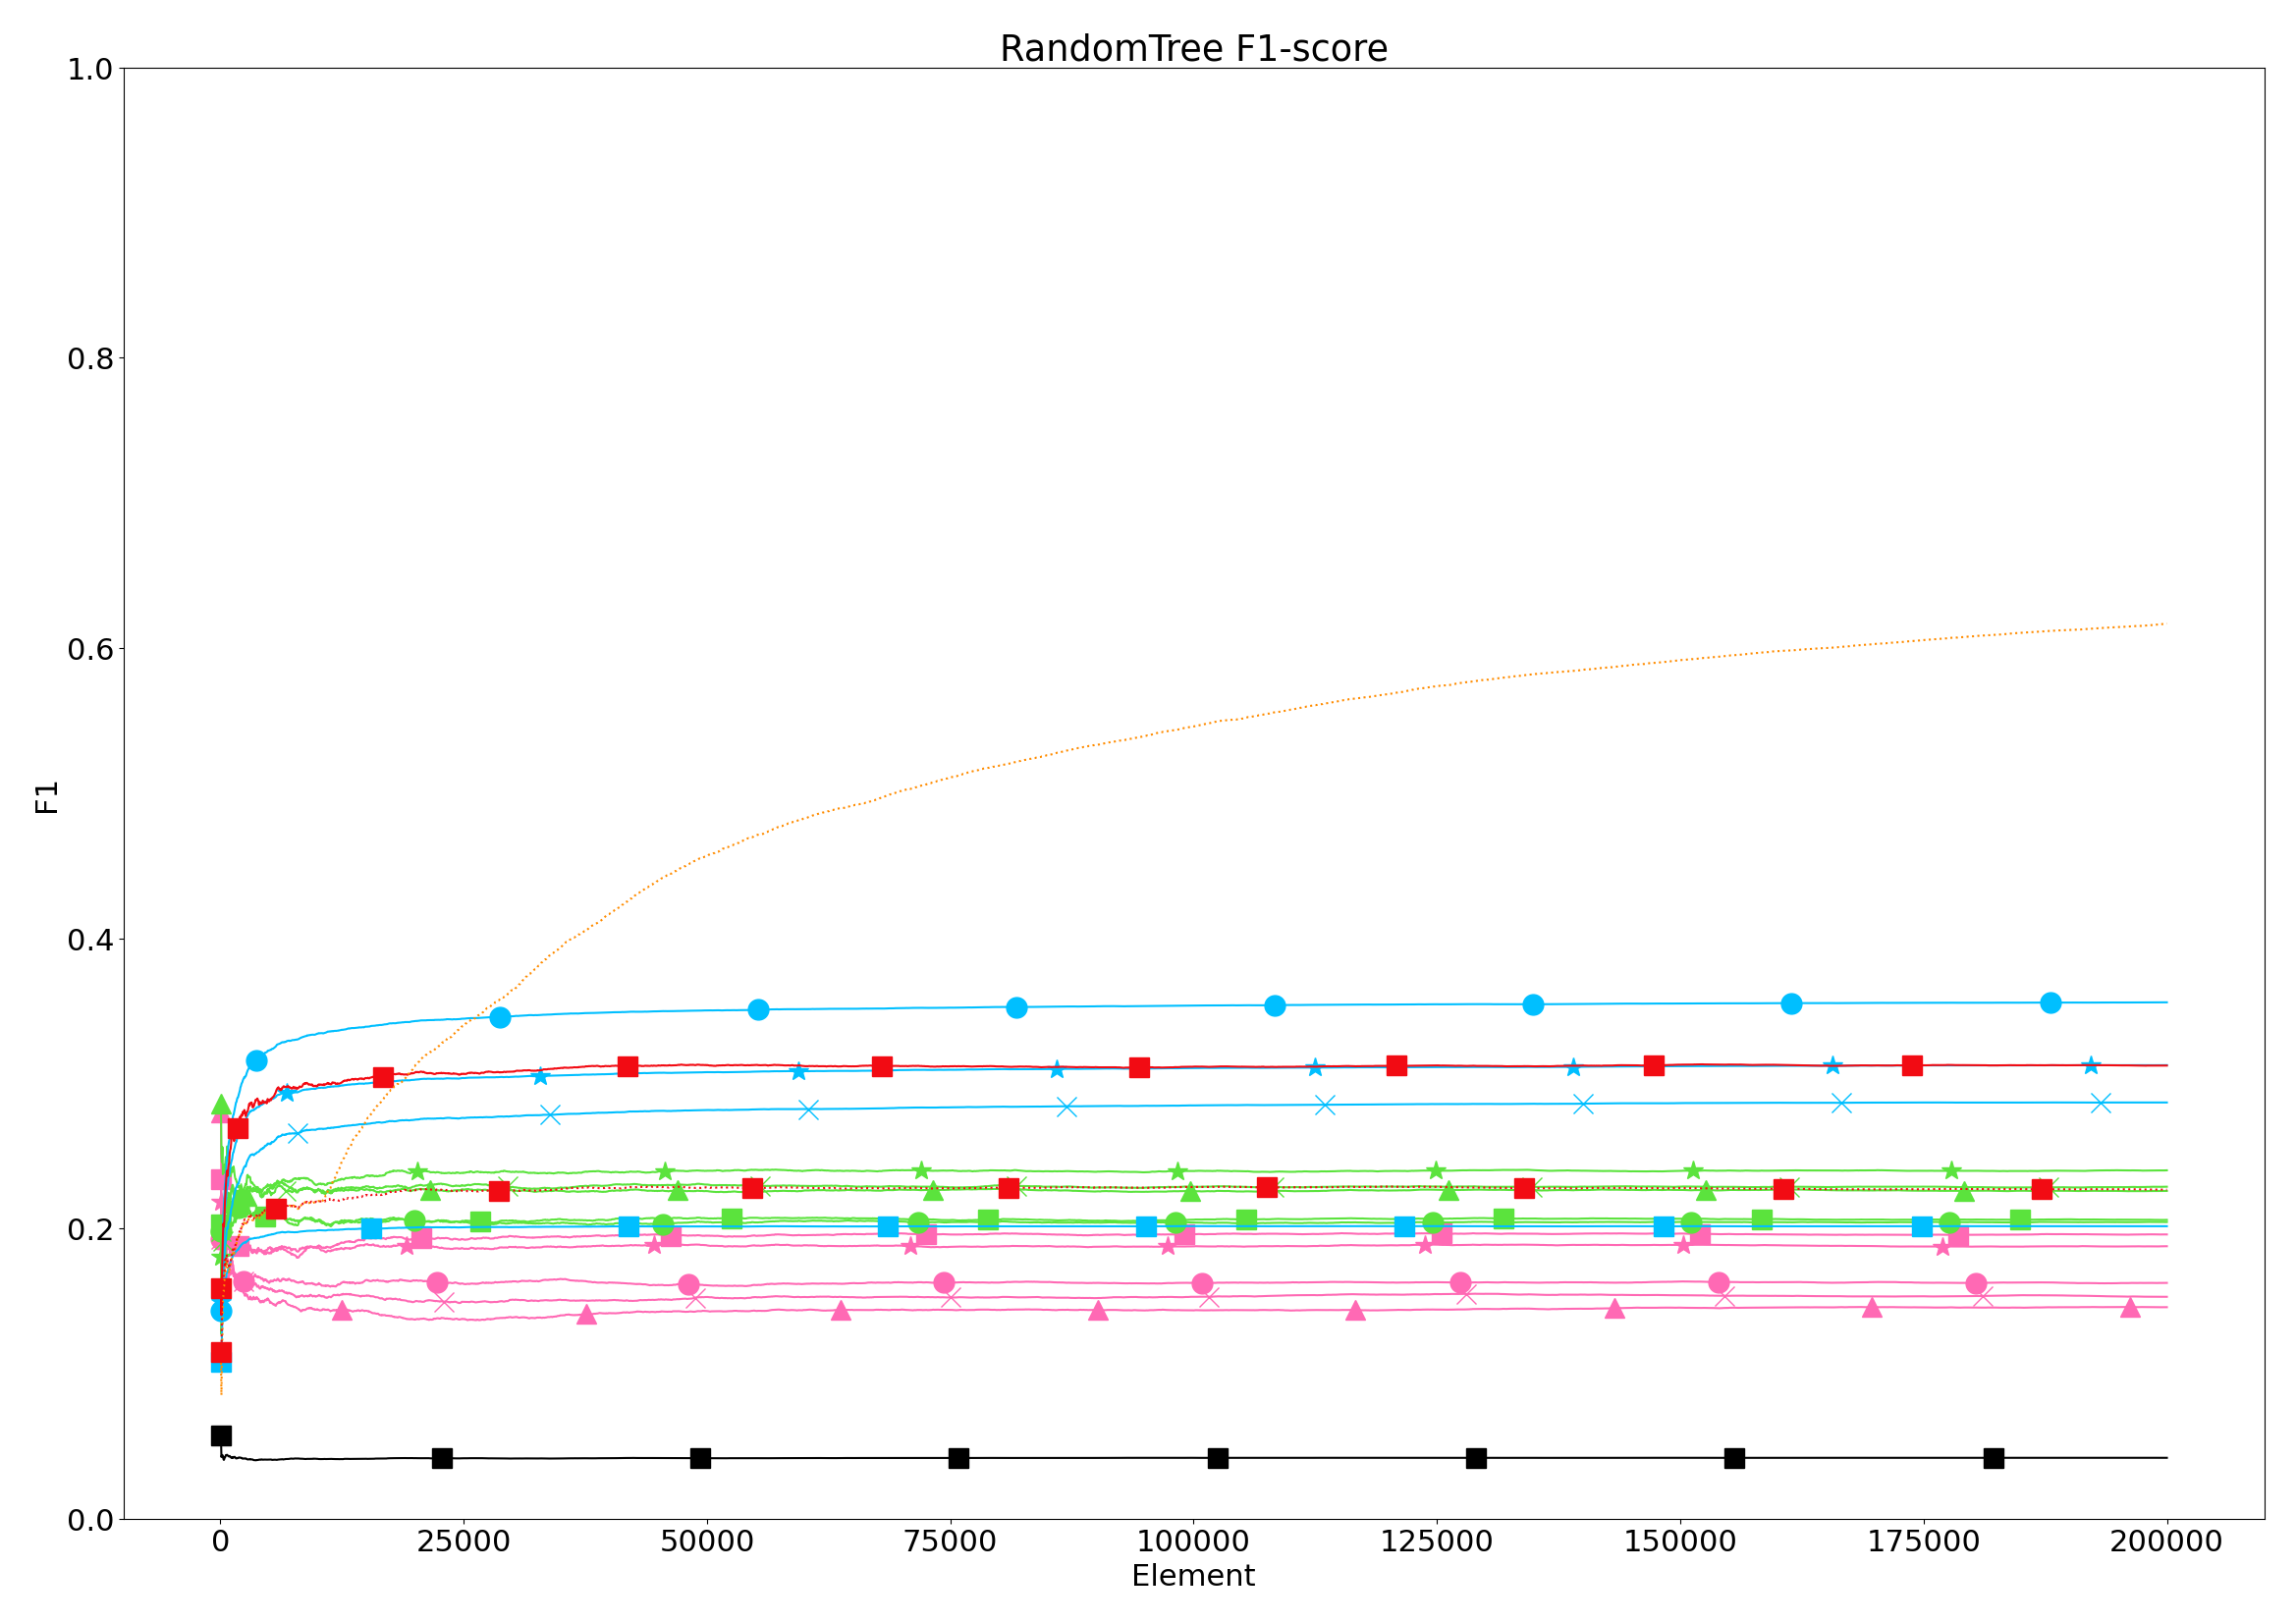
\includegraphics[width=\linewidth]{figures/results/dataset_3_f1.png}
		\caption{RandomTree (MOA)}
		\label{fig:f1-dataset_3}
	\end{subfigure}
	\begin{subfigure}[t]{.49\linewidth}
		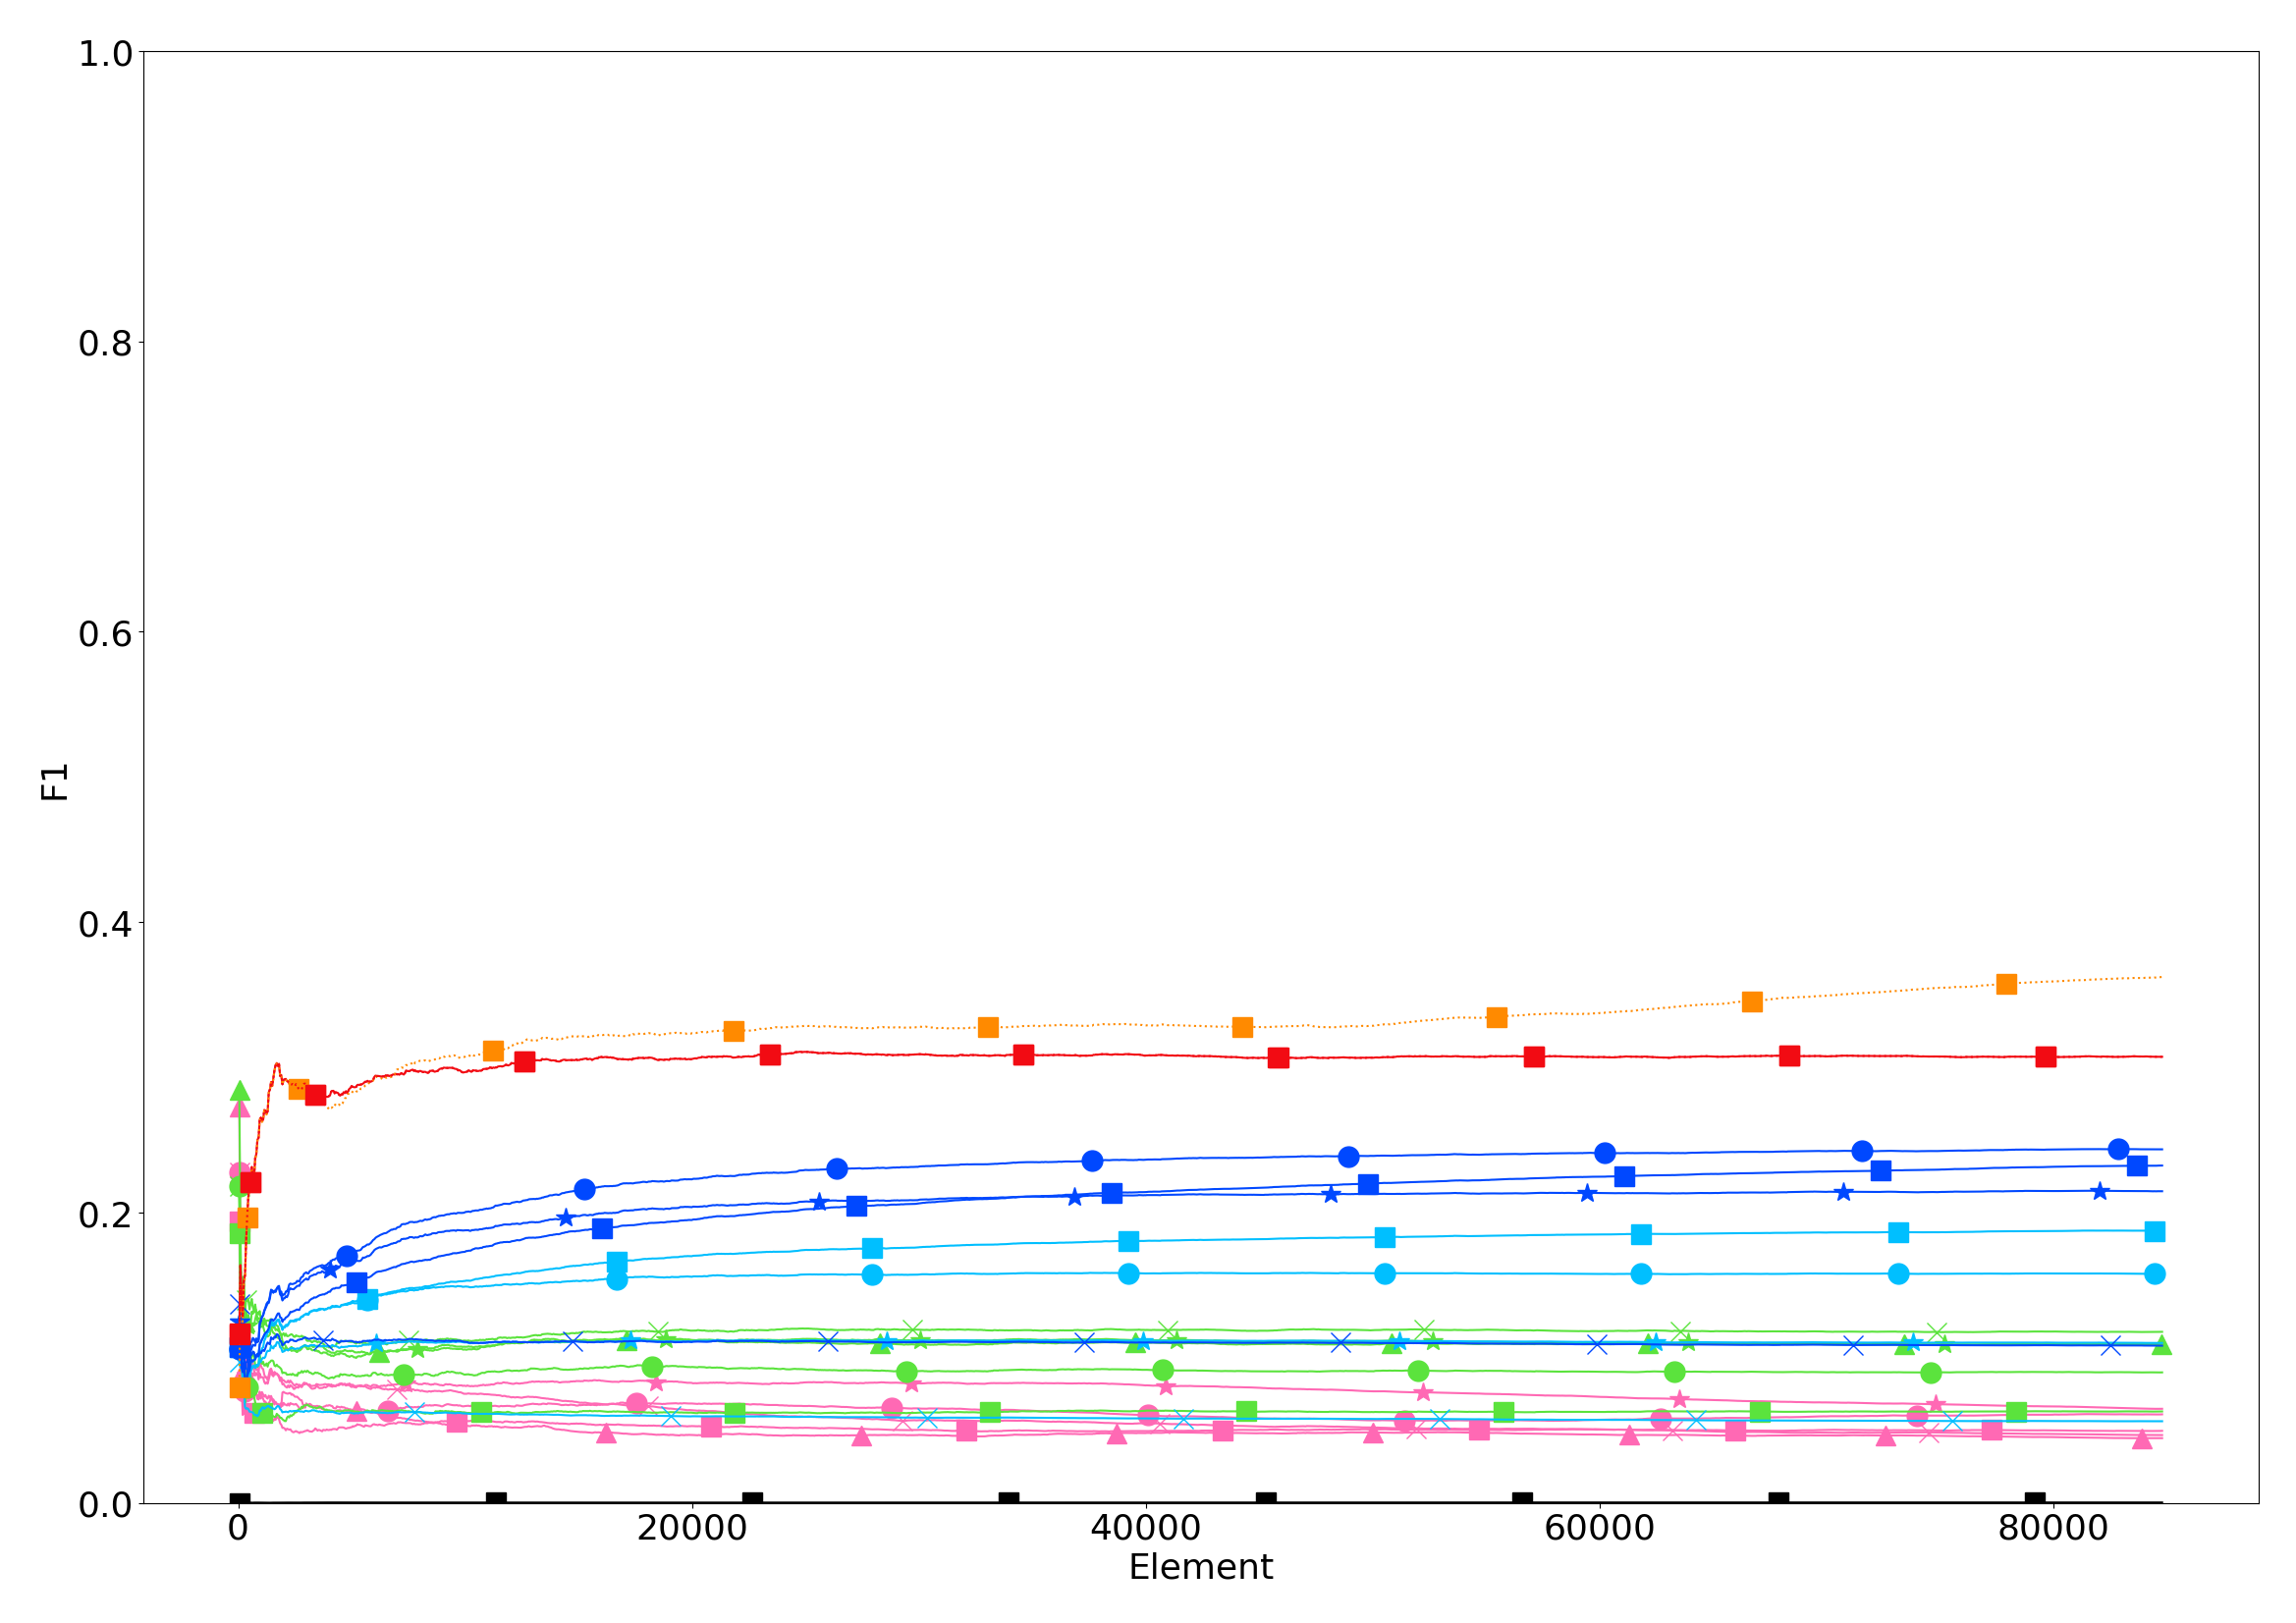
\includegraphics[width=\linewidth]{figures/results/recofit_6_f1.png}
		\caption{\recofitdataset}
		\label{fig:f1-recofit}
	\end{subfigure}
	\caption{F1-scores for the six datasets (average over 20 repetitions). The horizontal dashed green line indicate the offline KNN F1-score.}
	\label{fig:f1}
\end{figure*}

\section{Results}
This section presents our benchmark results and the corresponding
hyperparameter tunning experiments.

\subsection{F1-score}
Figure~\ref{fig:f1} compares the F1-scores obtained by all classifiers on the
six datasets.  \naivebayes and the \hoeffdingtree outperform the other
classifiers on the two real datasets (\banosdataset and \recofitdataset) even
though the F1-scores observed remained low (0.6 and 0.35) compared to offline
results (green horizontal line). On the other hand, the \mondrianforest (cyan)
with 5 or 10 trees achieves the best performances on 2 synthetic datasets.  The
\mondrianforest is also the third classifier on the two real datasets.
Finally, the \hoeffdingtree outperforms all other classifiers on the RandomTree
dataset, where it is followed by the \mondrianforest. We also note that the
\FNN remains better than \mcnn Origin but it is quite low compare to other
classifiers with the same dataset.

F1-score values vary greatly across the datasets.  While the highest
observed F1-score is above 0.95 on the Hyperplane and RandomRBF datasets,
it barely reaches 0.65 for the \banosdataset dataset, and it remains under
0.4 on the \recofitdataset and RandomTree datasets. This trend is
consistent for all classifiers.

The main difference between these datasets is the lower complexity of RandomRBF
and Hyperplane. Indeed, these two datasets have two classes with three
attributes while the others have at least ten classes. This suggest that the
number of classes may have an impact in the classification performance.

Figure~\ref{fig:f1-banos} includes the variance of the F1-score for
\mondrianforest classifiers, the only ones to involve randomness. The
variance decreases with the number of trees, as expected.
\TG{I dont find the last two sentences particularly
informative and this figure doesn't bring much at the end of the day. Could
you just add variance to figure 3?}.

The StreamDM \hoeffdingtree algorithm achieves better performance than the
\naivebayes except for the \banosdataset dataset.  Both of them start close
together because the \hoeffdingtree uses a \naivebayes in its leaves.  However,
they start diverging most likely because the \hoeffdingtree improves by reshaping its tree
structure.  This is caused by a sufficient amount of element and the difference
is more noticable when a concept drift occurs.

On all datasets, \mcnn OrpailleCC achieves better performances than \mcnn
Original. Presumably due to the fact that \mcnn Original removes clusters too
fast even with a low participation threshold.  Besides, on the real datasets
(\banosdataset and \recofitdataset), the \mcnn OrpailleCC classifier appears to
be learning faster than the \mondrianforest, although \mondrianforest catches
up after a few thousand elements. 

\subsubsection{\FNN}
Figure~\ref{fig:f1-banos} has shown that the \FNN has a low
F1-score compared to other classifiers. It contradicts the results
depicted in~\cite{omid_2019} where \FNN achieves more than 95\% 
accuracy. The main difference between~\cite{omid_2019} and this study comes
from the training set. In~\cite{omid_2019}, not only the training set includes examples from every
subjects, but also the windows are overlapping and wider than the ones we used.
Therefore, we expect the \FNN to have already encountered
most of the datapoints from the testing set. When instead of using only the
first subject of the \banosdataset dataset we used a sample of 10\% of of all datapoints in the \banosdataset dataset, we
managed to reach an F1-score slightly above 0.6, which is close to the \naivebayes.

Note that the pre-training of the \FNN is slightly different from the other
classifiers. Indeed, the hyperparameters tuning of the other classifiers
implies that they start the testing phase with no prior knowledge of the
dataset even about the element seen in the tuning phase. On the other hand, the
\FNN starts with its weights already set, therefore we can say that it has
already seen part of the dataset. We proceed that way because it takes many
epochs for the weights to adjust correctly so if the weights were randomly
initialized for the testing phase, the \FNN would answer randomly.

We deviated from the method for the \FNN classifier because neural networks have
shown a wide range of classification abilities depending on how they are used.
Therefore, we tried to follow~\cite{omid_2019} which exhibits high classification
performance.

\subsubsection{Bounded Memory}
Surprisingly, a \mondrianforest with 50 trees performs worse than with 5 or 10
trees on most datasets. The only exception is the Hyperplane dataset where
50 trees F1-score is between 5 and 10 trees. This is due to the fact that
our \mondrianforest implementation is memory bounded, which is
useful on connected objects but limits tree growth when the allocated memory is
full. Because 50 trees fill the memory faster than 10 or 5 trees, the
classifier learning is blocked faster, when the trees have not learned enough
from the data.
We differentiate bounded memory from constant space complexity because in the
first case, a limited amount of memory may force the classifier to find a way
around this lack of memory: stop growing or making space for new data.
Therefore, influencing its performance.  On the other hand, a constant space
complexity is a feature of a classifier and its performances are not expected
to change no  matter the amount of memory available. The classifier is simply
supposed to fail without the required amount of memory. From the algorithm
involved in this study, \mondrianforest has a bounded memory policy while
\naivebayes is a classifier with a constant space complexity.

This dependency of the \mondrianforest to memory allocation is shown in
Figures~\ref{fig:f1-banos}-\ref{fig:f1-recofit}, where an additional
configuration with five time more memory (total of 3MB) is shown (deep blue).  The memory
increase induces a F1-score difference greater than 0.1, except when only one
tree is used. In which case the improvement caused by the memory is less than
0.05.

Note that the selected the memory bound does not match all situations. Indeed,
depending on the connected object the memory limit can range from few KB to GB.
In this study, the \mondrianforest is limited to 600~KB.

The \hoeffdingtree appears to be the most robust to concept drifts
(Figure~\ref{fig:f1-drift}), while the \mondrianforest and \naivebayes
classifiers are the most impacted. \mcnn classifiers are only marginally impacted.
The low resilience of \mondrianforest to concept drifts can be attributed to
two factors. First, existing nodes in trees of a \mondrianforest cannot be updated.
Second, when the memory limit is reached, \mondrianforest cannot grow
or reshape their structure anymore.

Figure~\ref{fig:f1-banos} shows that the F1-score of the \FNN
is around 0.3 \TG{Why isn't it shown in the other figures?}. 

Finally, we note that the StreamDM and OrpailleCC implementations of
\naivebayes are indistinguishable from each other, which confirms our
implementation in OrpailleCC.

In this study, we focused on using one sensor rather than all the sensors
available in the real datasets. In the case of more sensor used, we would
expect an F1-score improvement for all classifiers because they would have
access to more data in order to discriminate the classes. On the other hand we
would expect an increase in the memory footprint because more sensors means
more attribute extracted. This should have minimal impact on classifier such as
\naivebayes because their footprint is already low. However, the
\mondrianforest, the \hoeffdingtree, and \mcnn memory footprints are expected to grow
significatively because more sensors means more attributes for each leaf or cluster.

\begin{figure*}
	\begin{subfigure}[t]{.49\linewidth}
		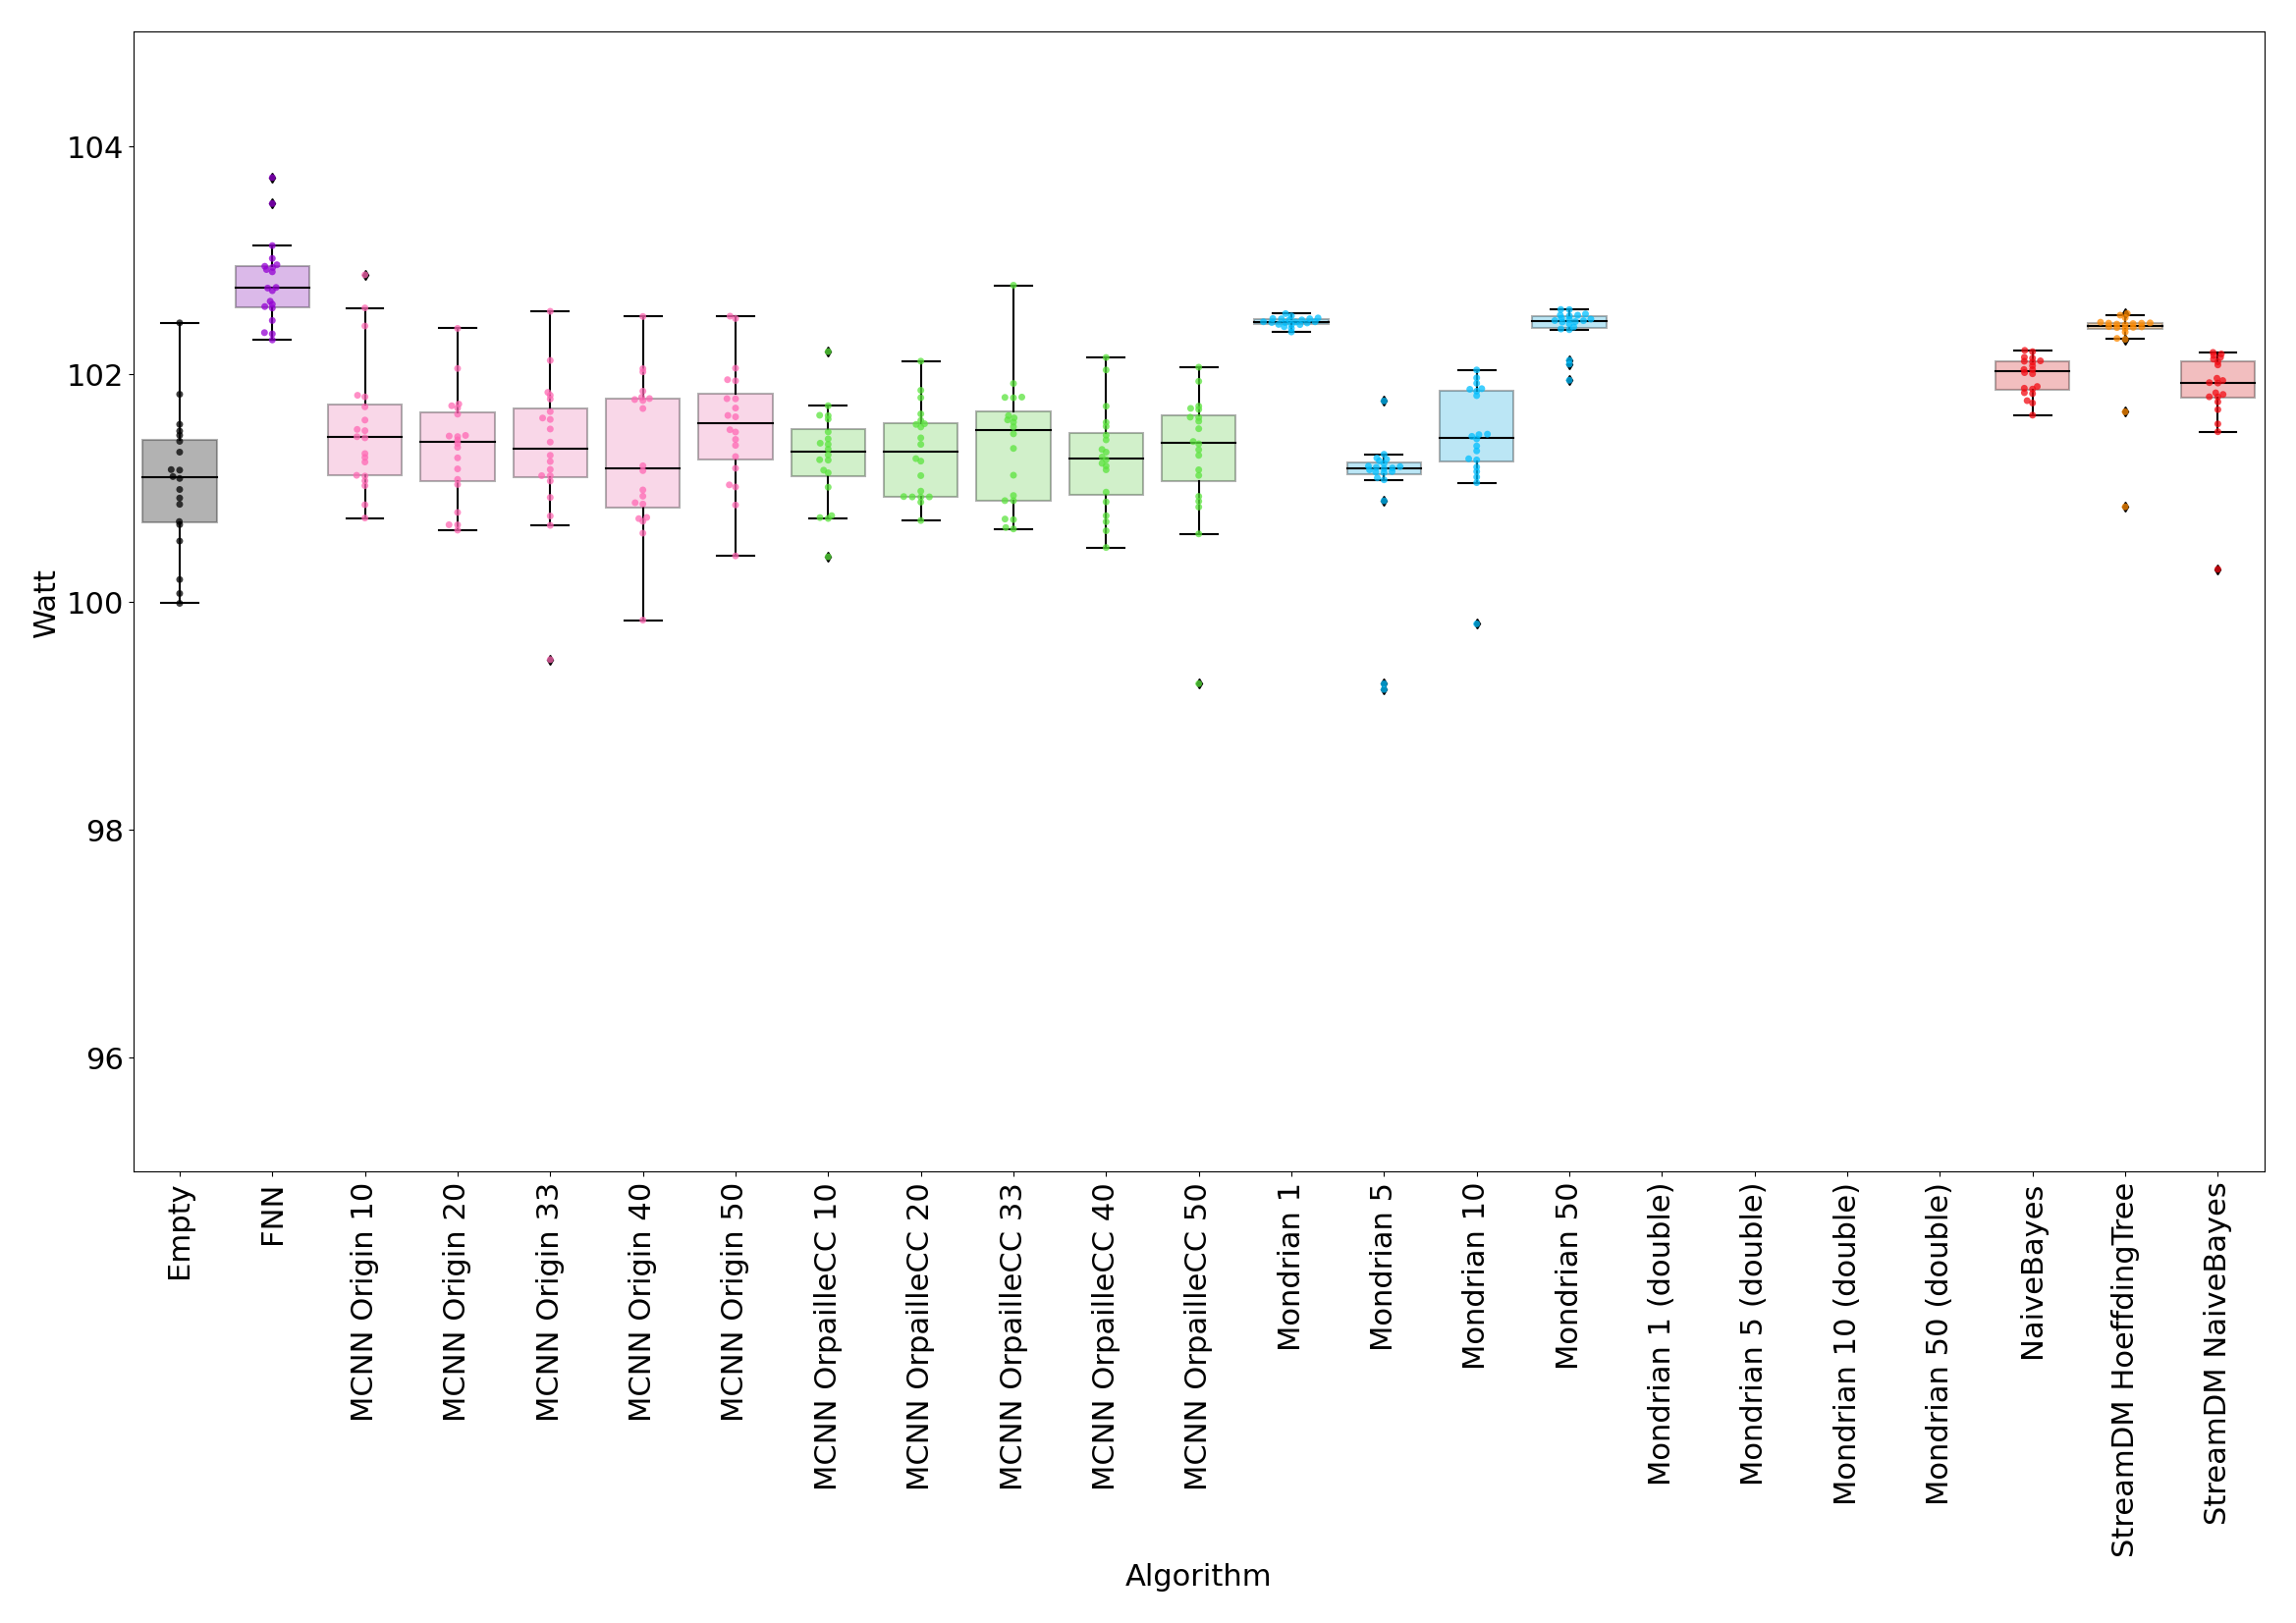
\includegraphics[width=\linewidth]{figures/results/banos_3_watt.png}
		\caption{\banosdataset}
		\label{fig:power-banos}
	\end{subfigure}
	\hfill
	\begin{subfigure}[t]{.49\linewidth}
		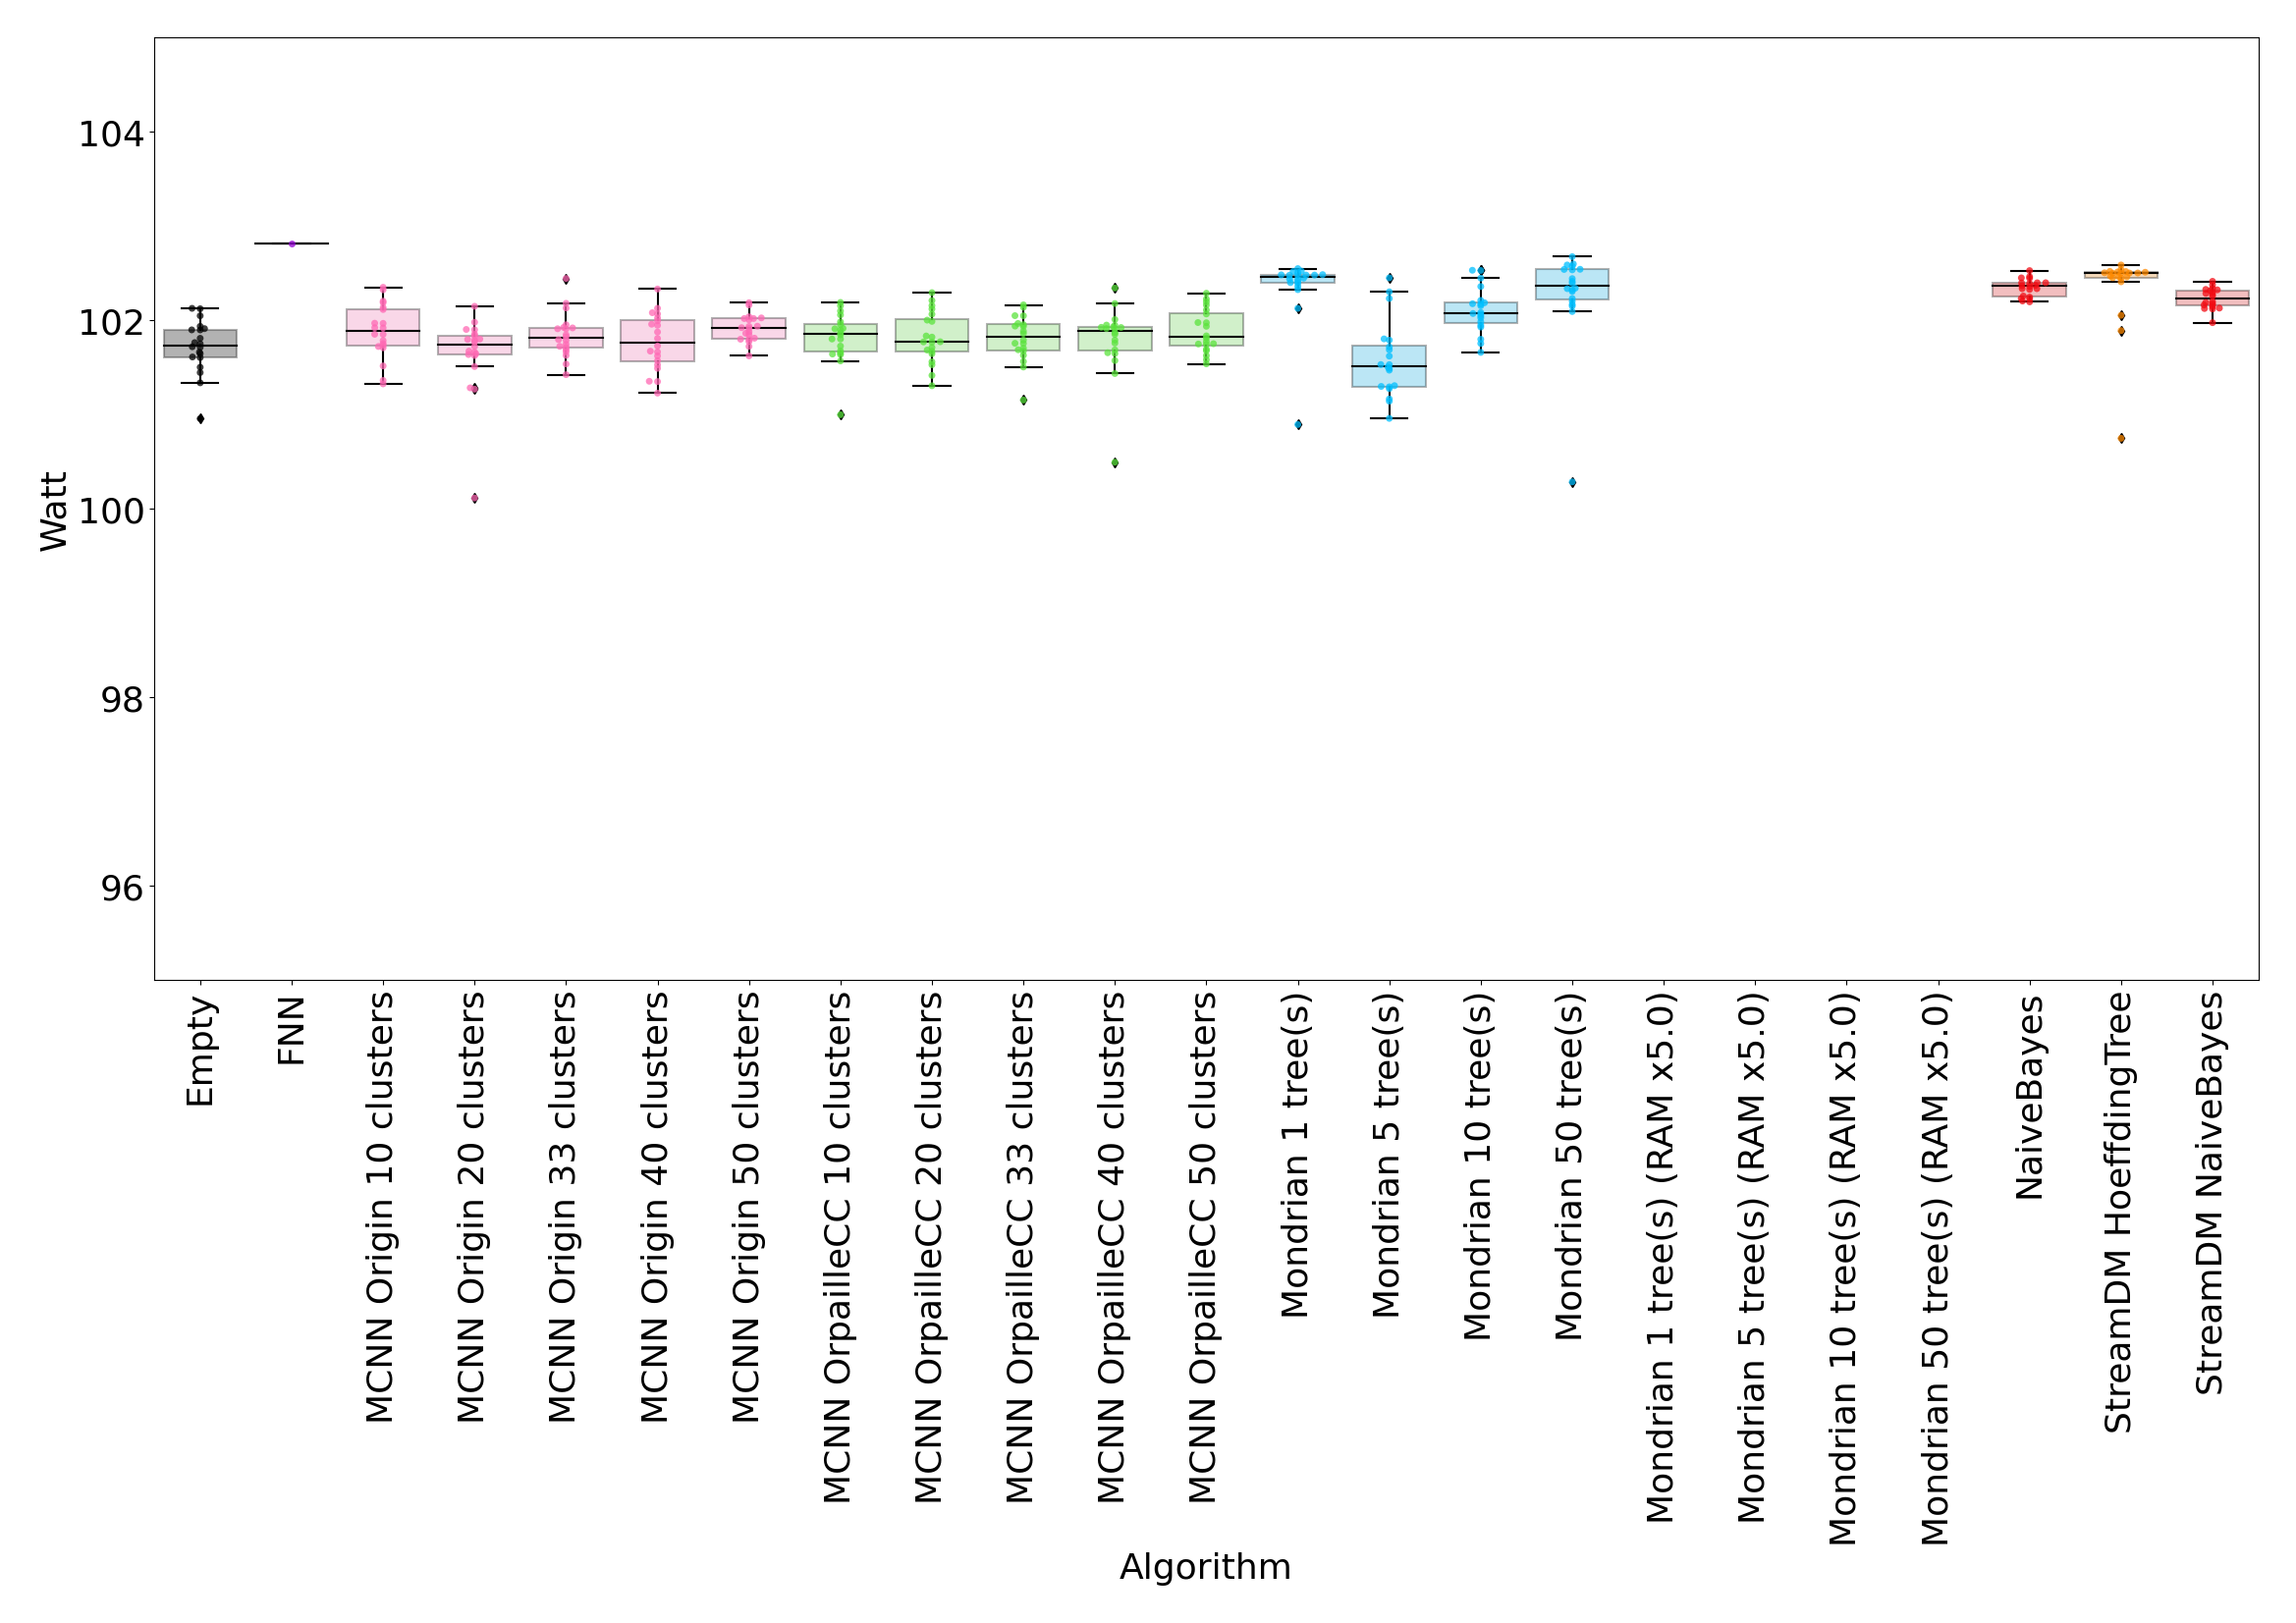
\includegraphics[width=\linewidth]{figures/results/drift_6_watt.png}
		\caption{\banosdataset with drift.}
		\label{fig:power-drift}
	\end{subfigure}\\
	\begin{subfigure}[t]{.49\linewidth}
		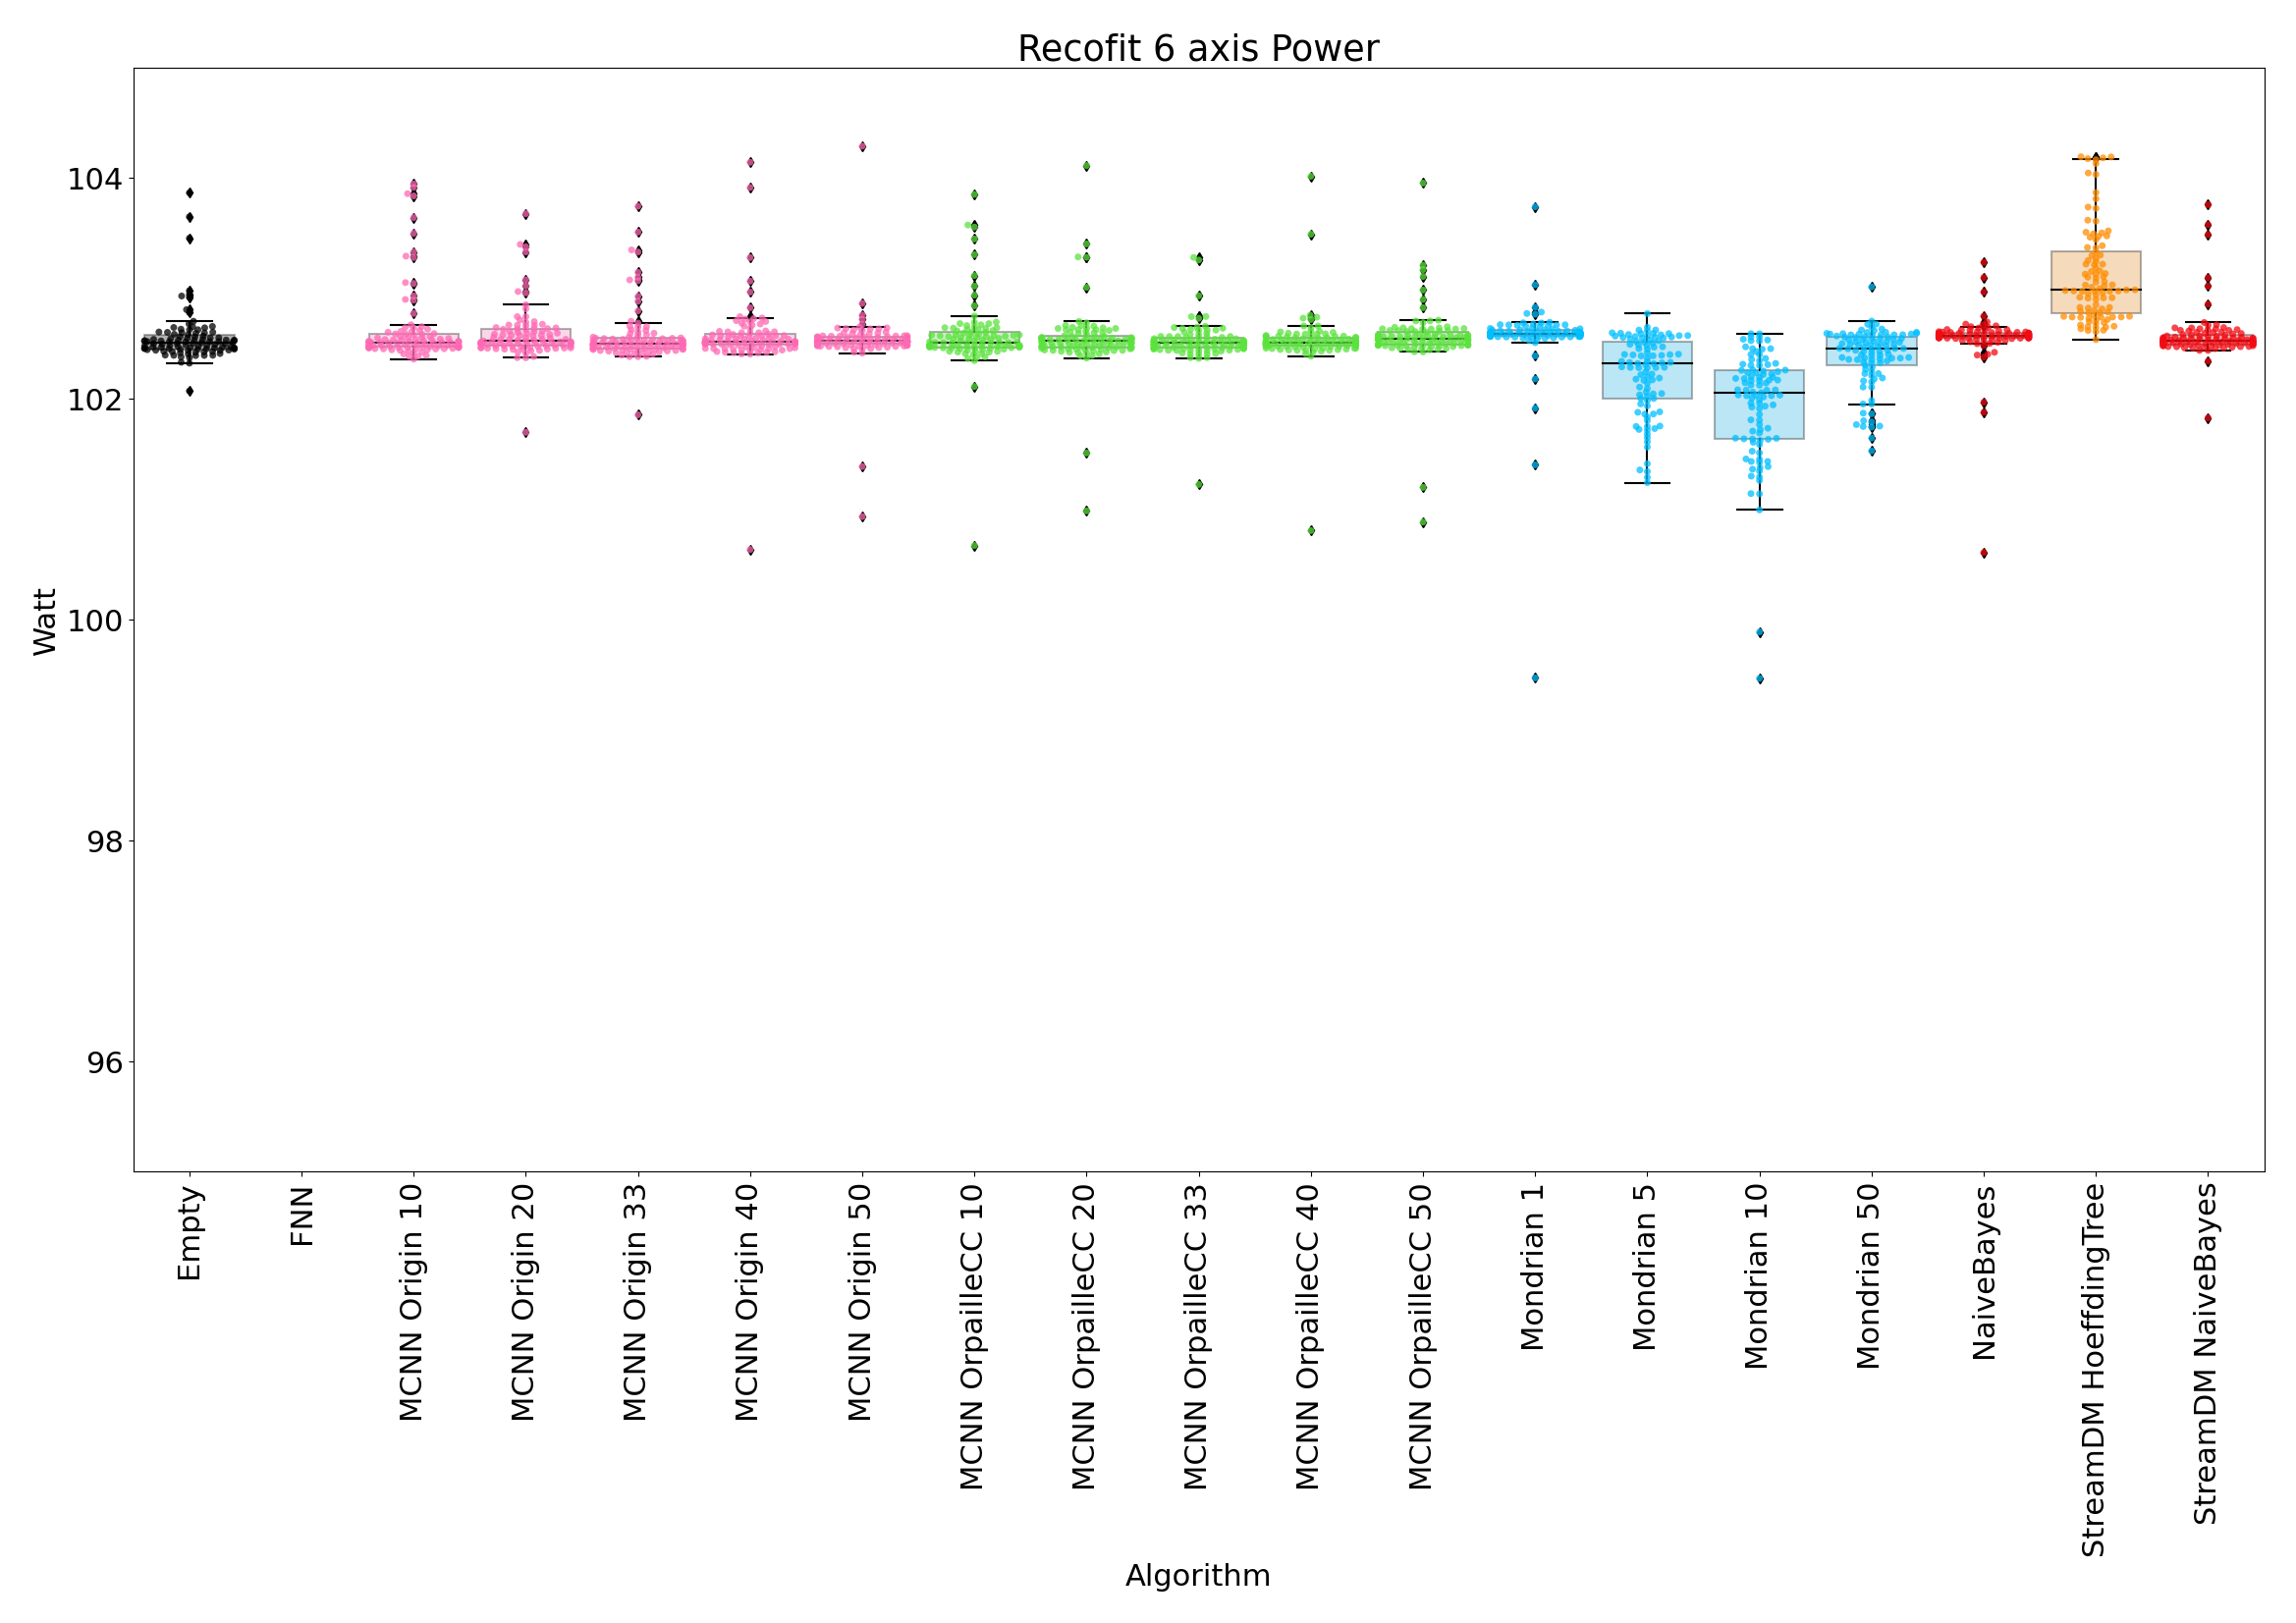
\includegraphics[width=\linewidth]{figures/results/recofit_6_watt.png}
		\caption{\recofitdataset}
		\label{fig:power-recofit}
	\end{subfigure}
	\hfill
	\begin{subfigure}[t]{.49\linewidth}
		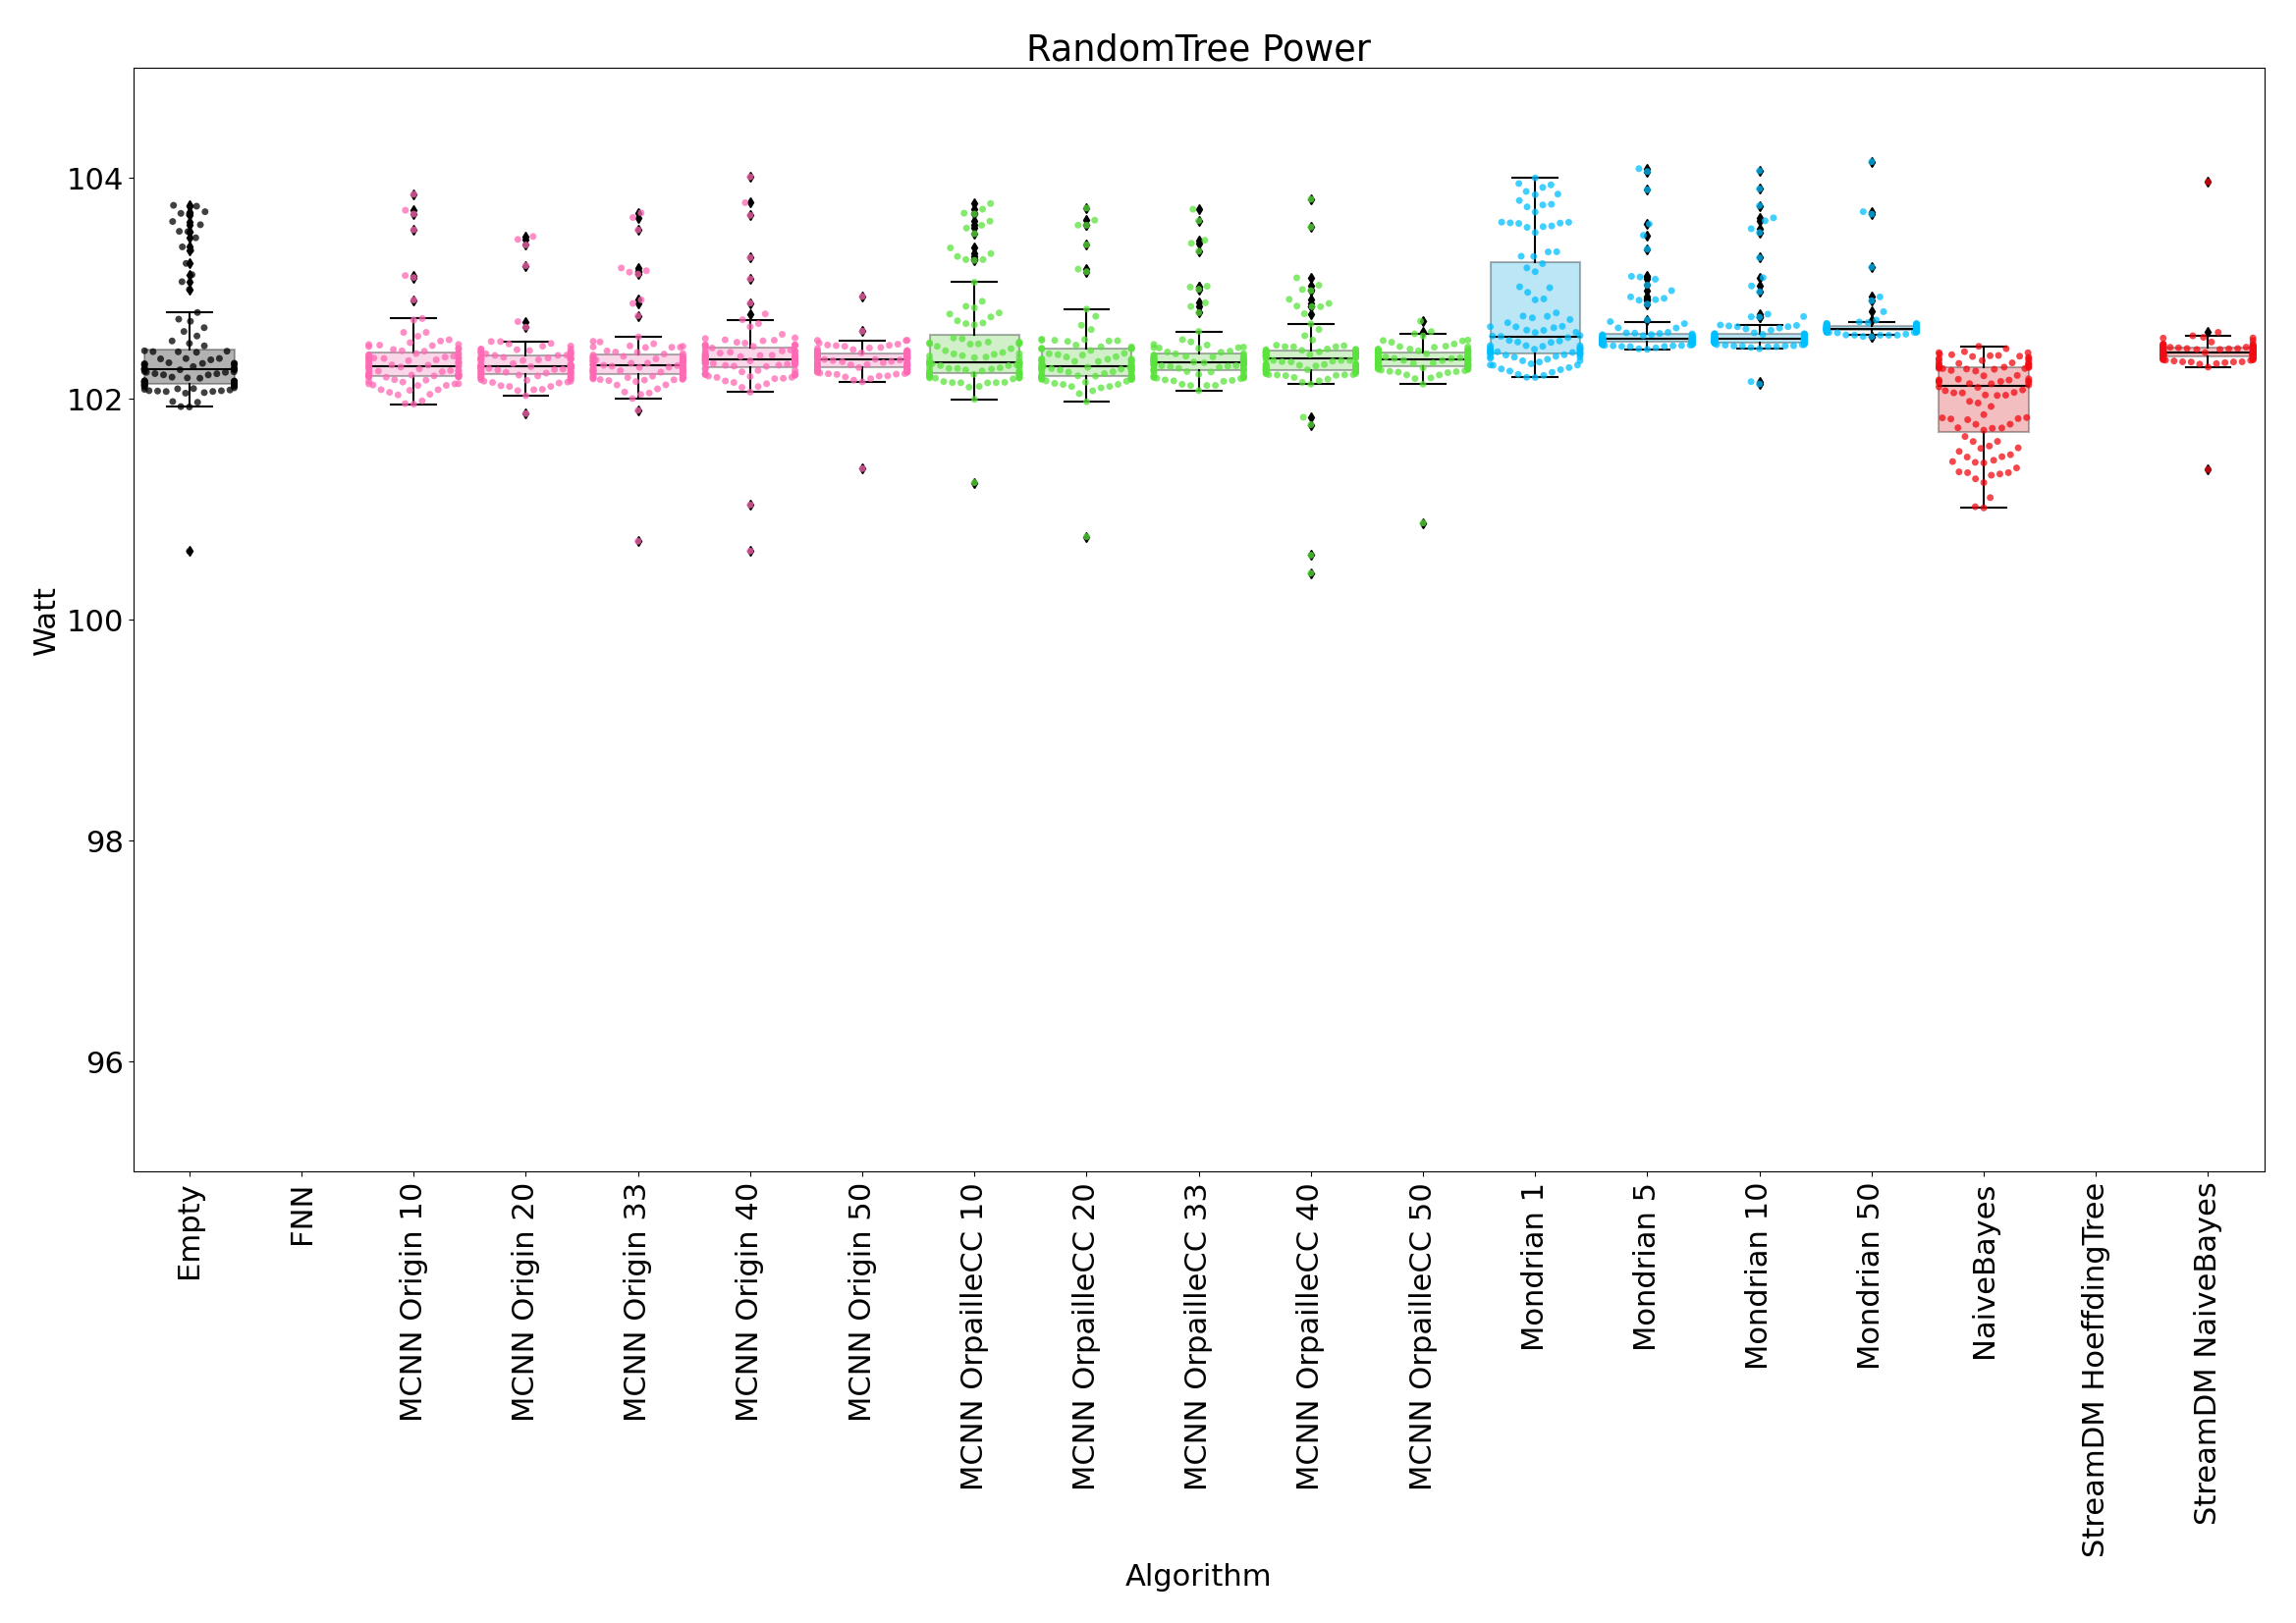
\includegraphics[width=\linewidth]{figures/results/dataset_3_watt.png}
		\caption{RandomTree}
		\label{fig:power-dataset_3}
	\end{subfigure}
	\caption{Power usage for four datasets.}
	\label{fig:power}
\end{figure*}
\subsection{Power}
\label{sec:result-power}
Figure~\ref{fig:power} shows the power usage of each classifier on four
datasets. Since all classifiers exhibit comparable power consumptions, close to
102~W, we decided to show only four of them. Figure~\ref{fig:power-drift} also
shows that the concept drift does not influence the power consumption.

This observation is explainable by two factors. The platform used is too powerful
and it was already working at minimal power. Indeed, to ensure no disturbance
by a background process, we run the classifier on an isolated cluster node with
eight cores. Therefore, the power difference on one core is not noticeable.

Another reason is the dataset size. Indeed, the slowest run is about
10 seconds with 50 Mondrian trees on \recofitdataset dataset.  Such short
execution does not leave the time for the CPU to switch P-states because it
barely warms a core.
\TG{you should explain why your results are still relevant and how they are expected to generalize on 
connected objects.}


\subsection{Runtime}
Figure~\ref{fig:runtime} shows the runtime of classifiers for the two real
datasets. The
\mondrianforest is the slowest classifier, in particular for 50 trees. The
second slowest classifier is the \hoeffdingtree, with a runtime comparable to the
\mondrianforest with 10 trees. The \hoeffdingtree is followed by the two \naivebayes
implementations, which is not surprising since \naivebayes classifiers are used
in the leaves of the \hoeffdingtree. The \mcnn classifiers are the fastest
ones, with a runtime very close to the empty classifier.

We observe that the runtime of StreamDM's \naivebayes is comparable to
 OrpailleCC's. This suggests that the performance of the two
 libraries is similar, which justifies our comparision of \hoeffdingtree
 and \mondrianforest.

\begin{figure*}
	\begin{subfigure}[t]{.49\linewidth}
		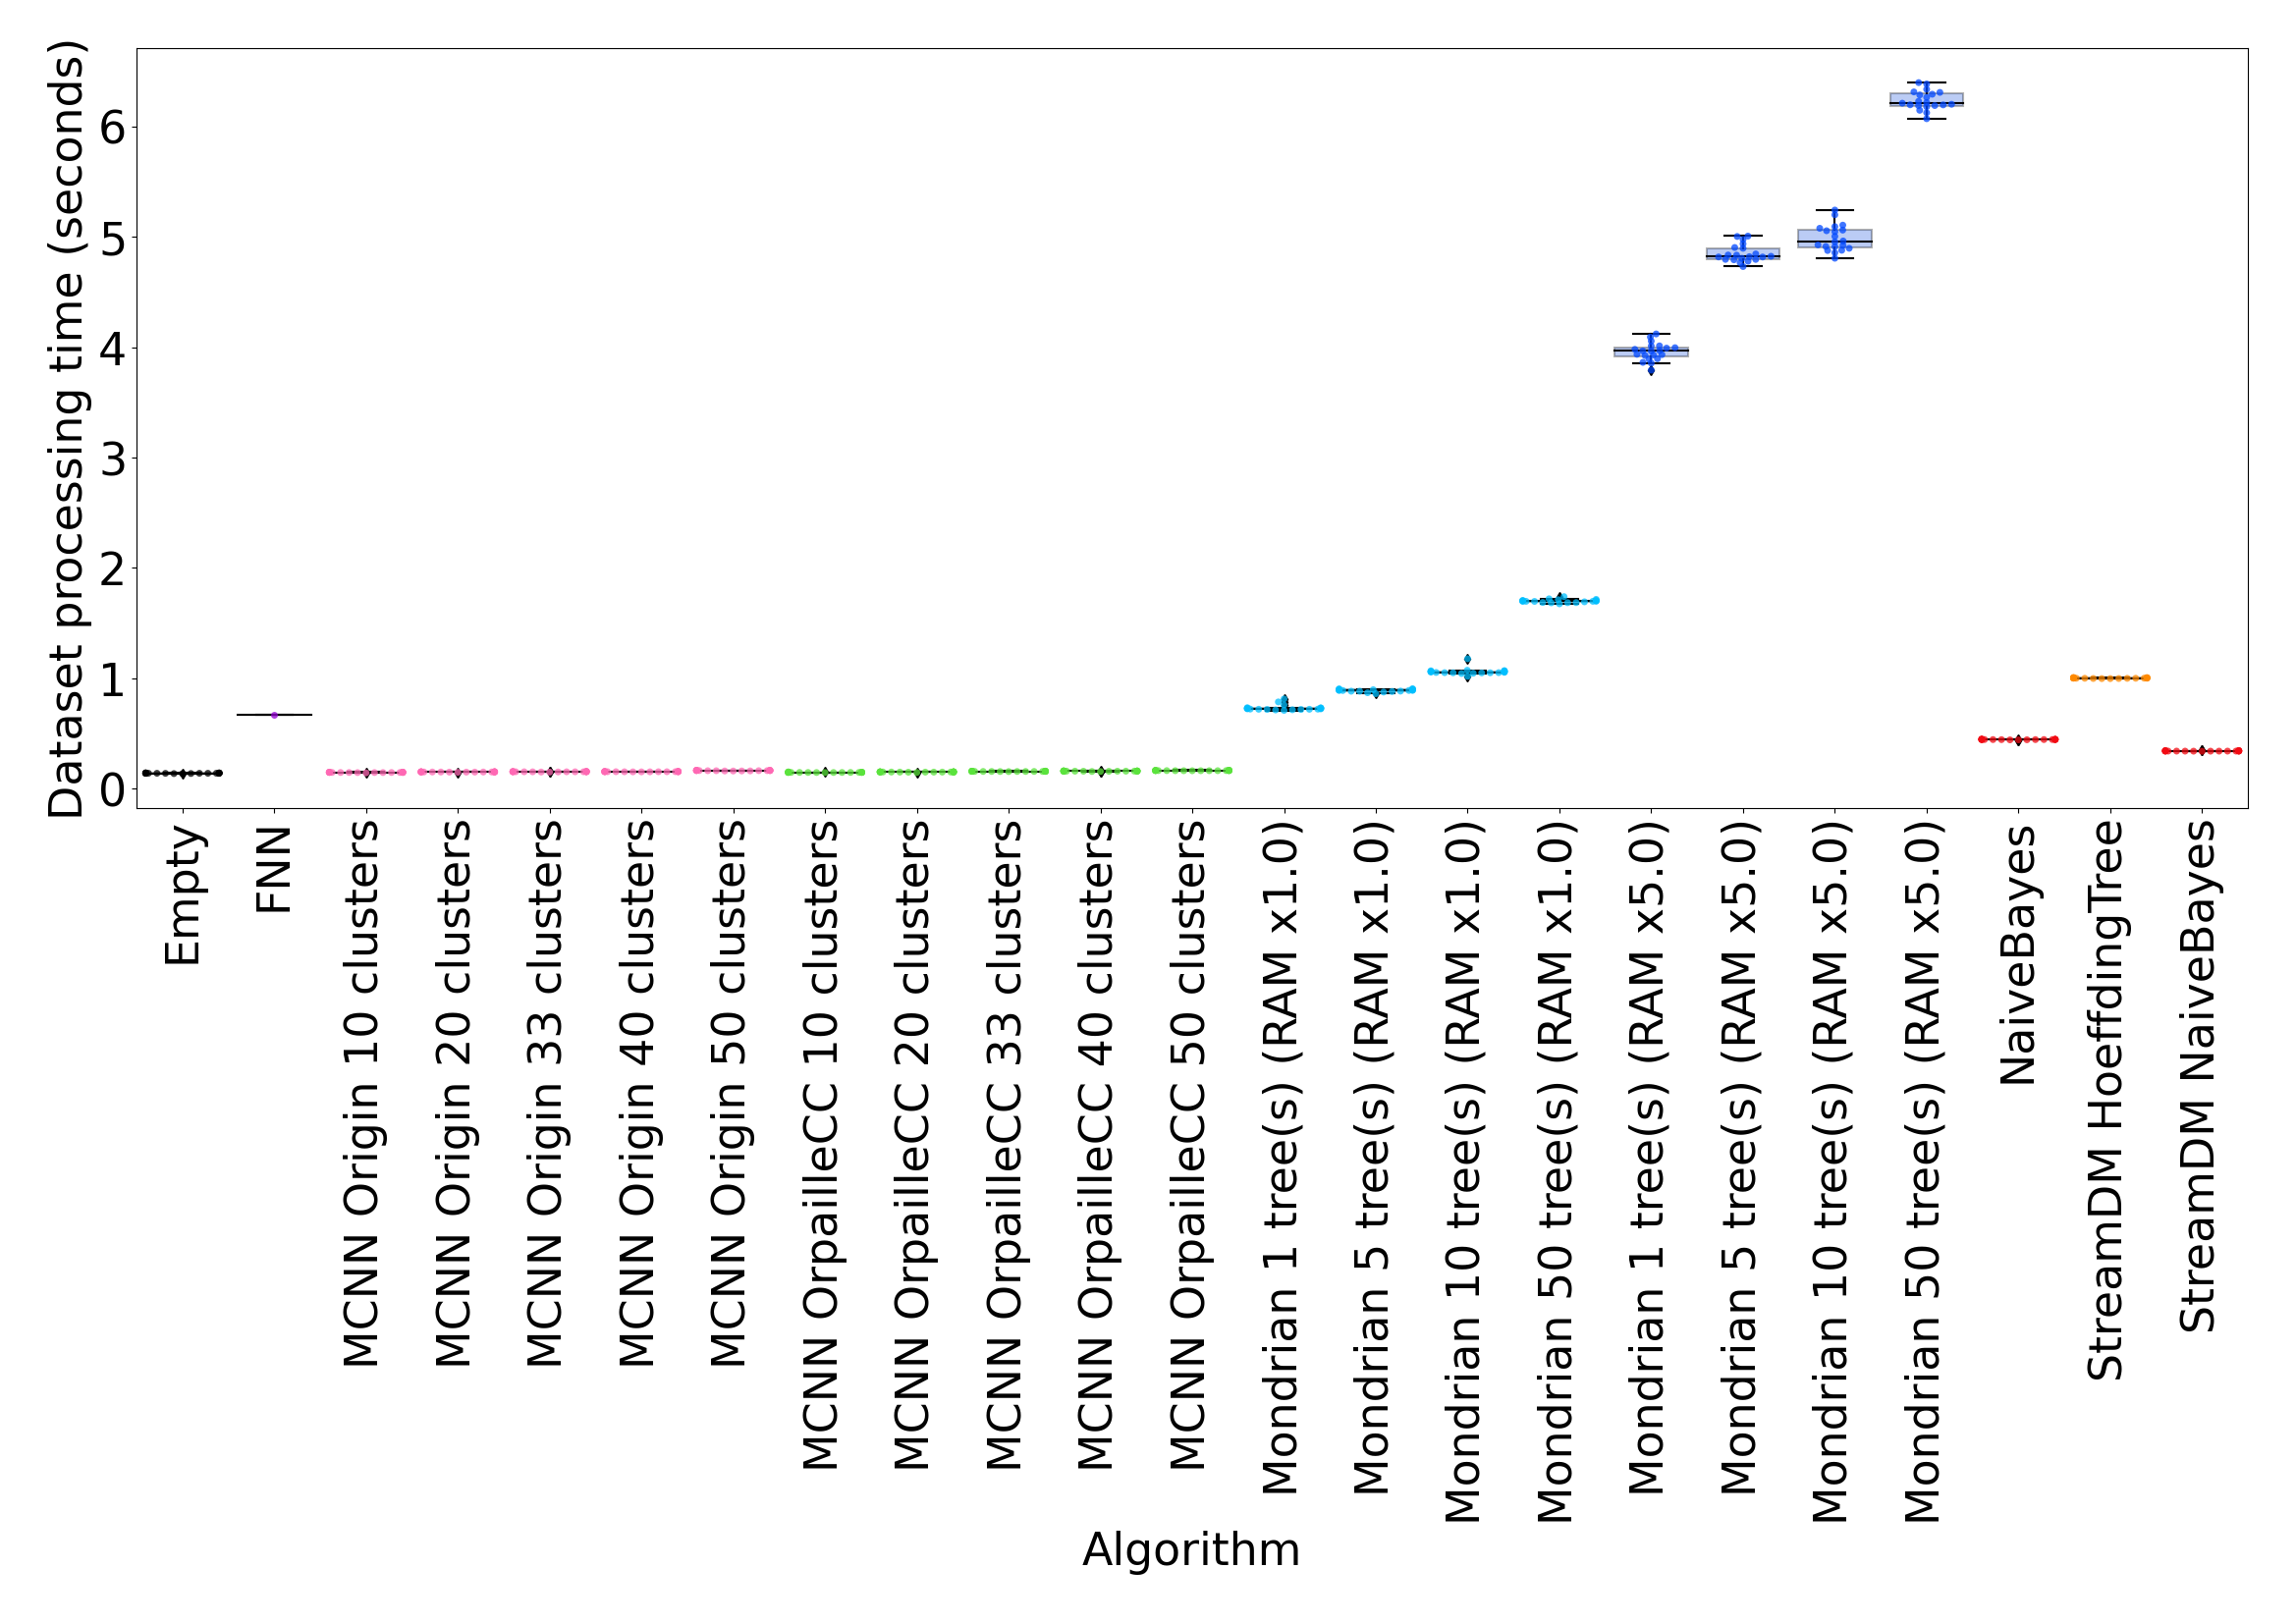
\includegraphics[width=\linewidth]{figures/results/banos_6_runtime.png}
		\caption{\banosdataset}
		\label{fig:runtime-banos}
	\end{subfigure}
	\hfill
	\begin{subfigure}[t]{.49\linewidth}
		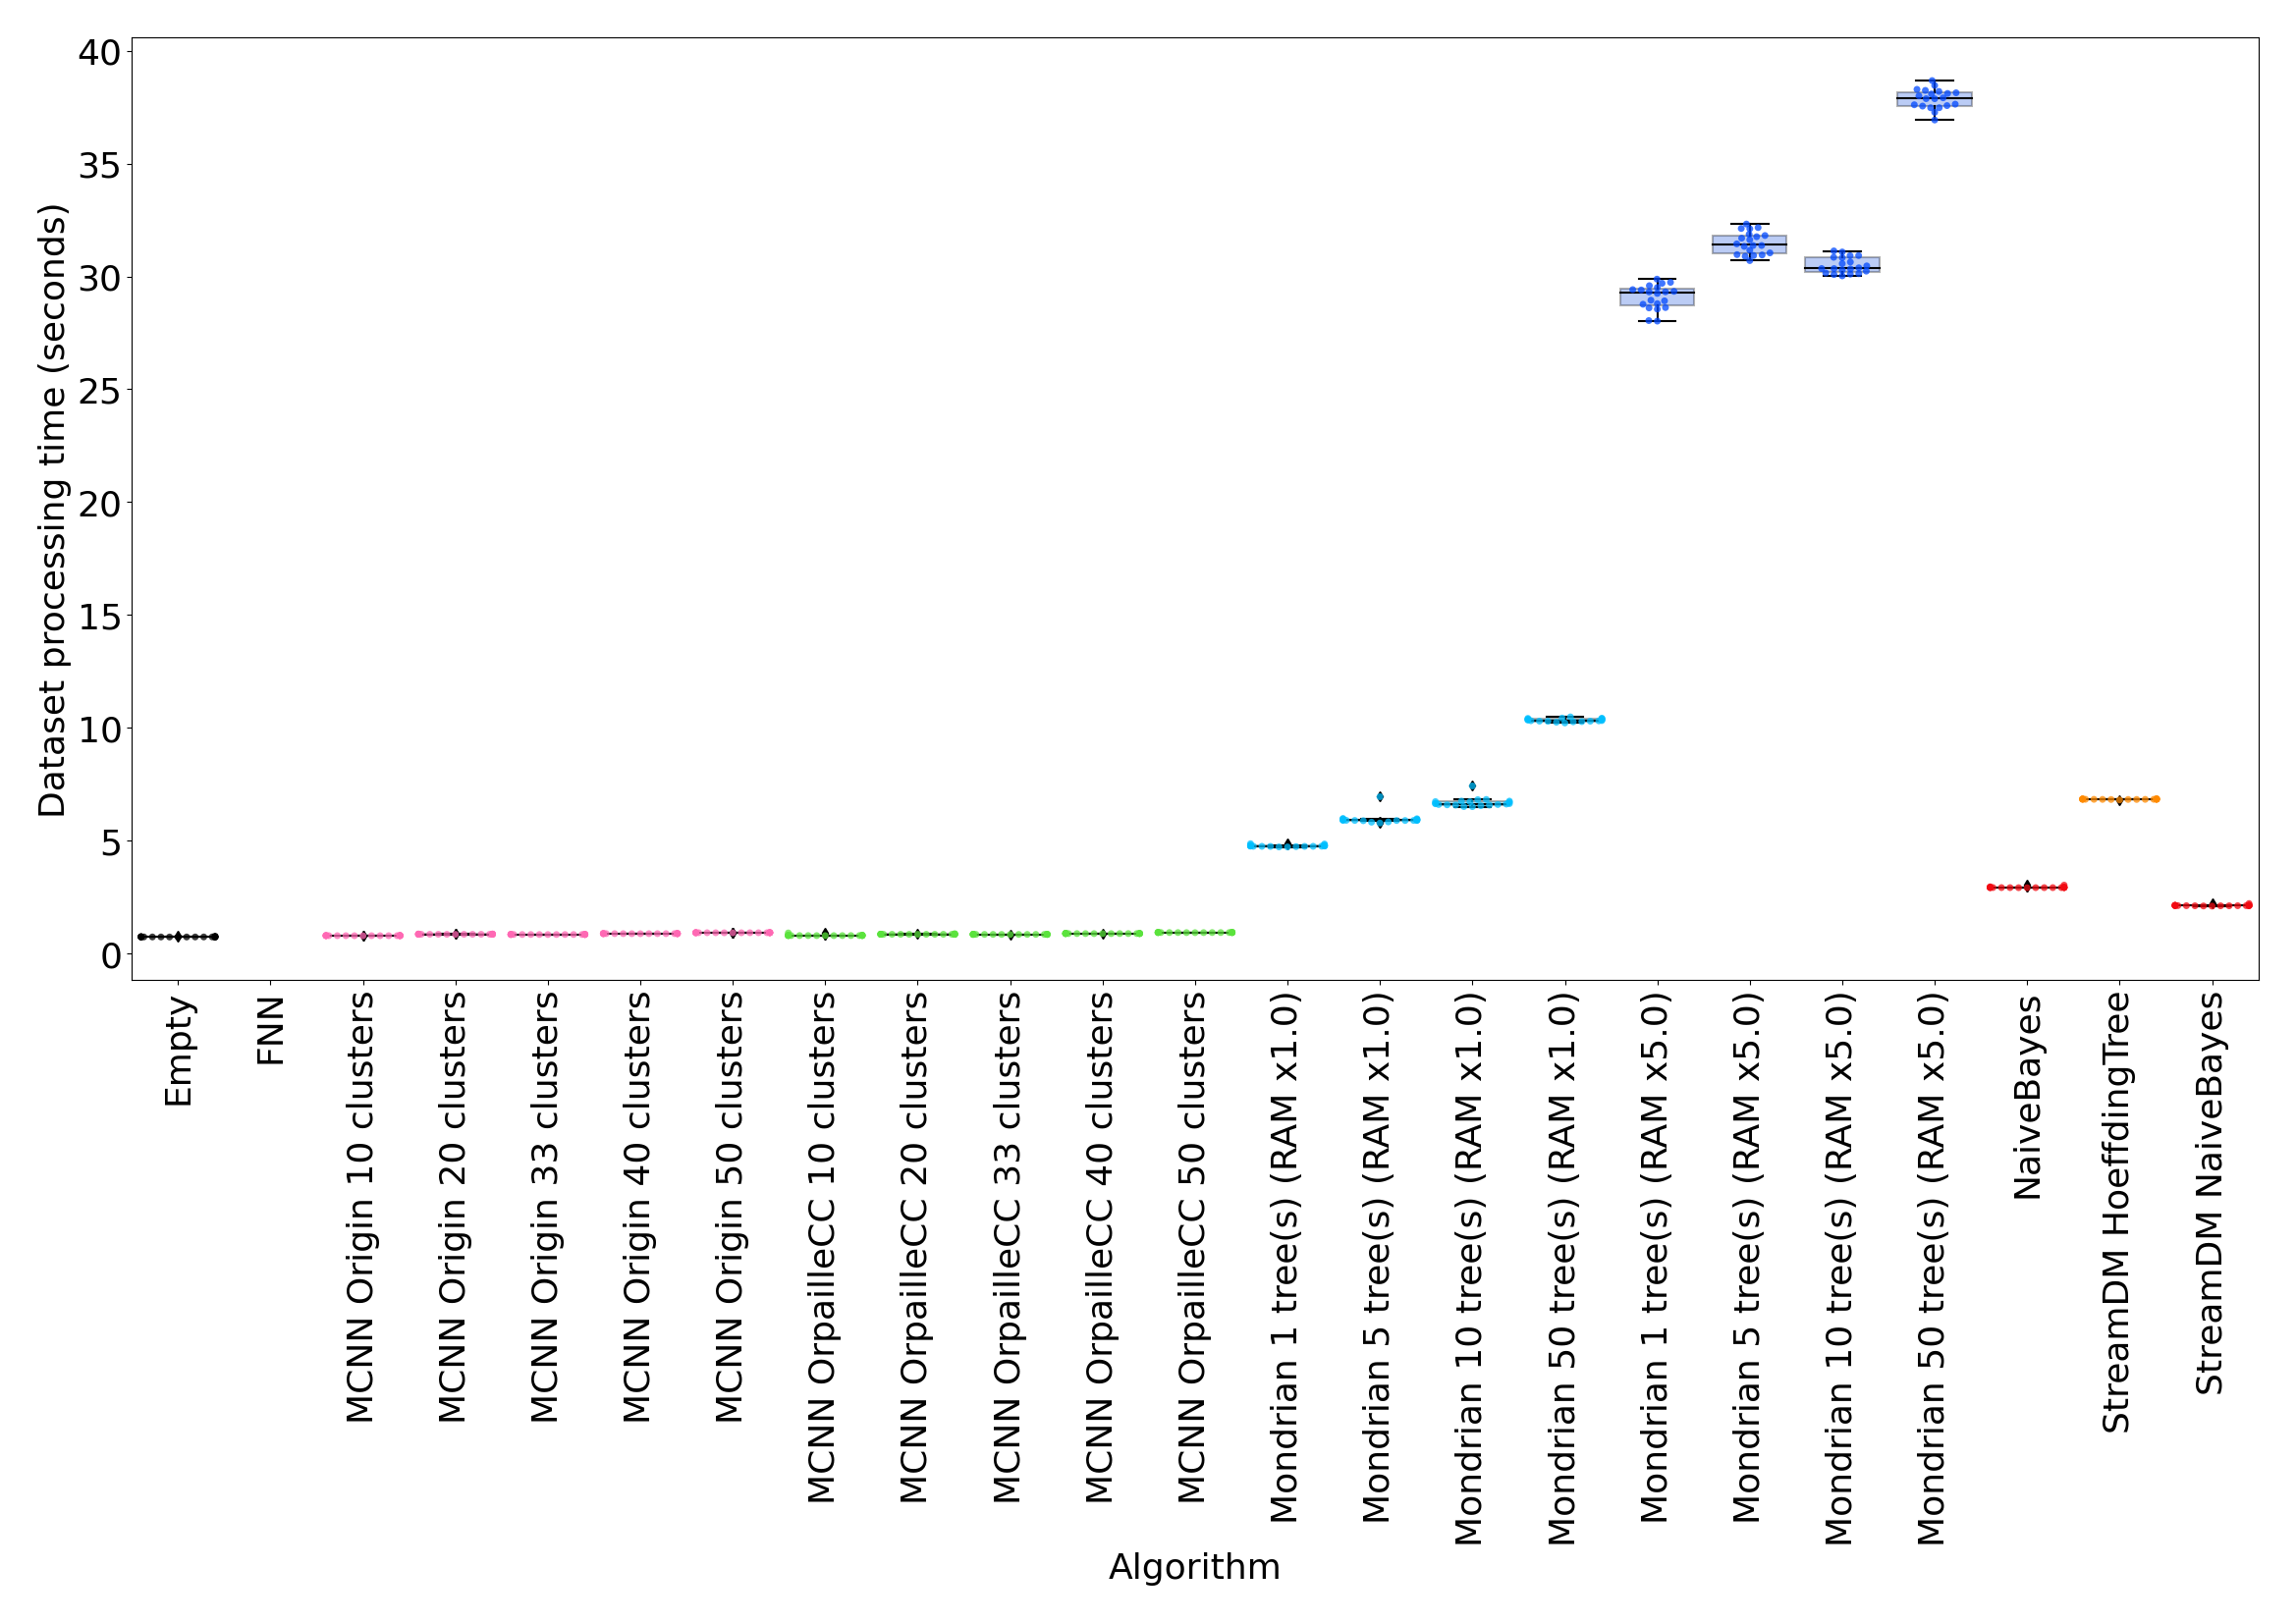
\includegraphics[width=\linewidth]{figures/results/recofit_6_runtime.png}
		\caption{\recofitdataset}
		\label{fig:runtime-recofit}
	\end{subfigure}
	\caption{Runtime with the two real datasets (20 repetitions).}
	\label{fig:runtime}
\end{figure*}

\subsection{Memory}
\label{sec:result-memory}
Figure~\ref{fig:memory} shows the evolution of the memory footprint for the
\banosdataset dataset. Because we focus on the classifiers footprint, the
figure only shows the memory difference between the classifiers and the empty
classifier. 

Memory footprint is similar across all datasets and all classifiers, due to the
fact that most algorithms follow a bounded memory policy or have a constant
space complexity.  The only exception is the \hoeffdingtree that constantly
selects new splits depending on new data points. The \mondrianforest has the
same behavior but the OrpailleCC implementation includes a memory bound, which
makes its memory footprint constant. Note that the concept drift does not
increase the memory footprint of the \hoeffdingtree.


\TG{it looks like the hoeffding tree consumes way more memory, but isnt it a
side effect of using streamDM? Maybe all memory consumptions should be computed by reference 
to the naive bayes baseline. }

\begin{figure}
	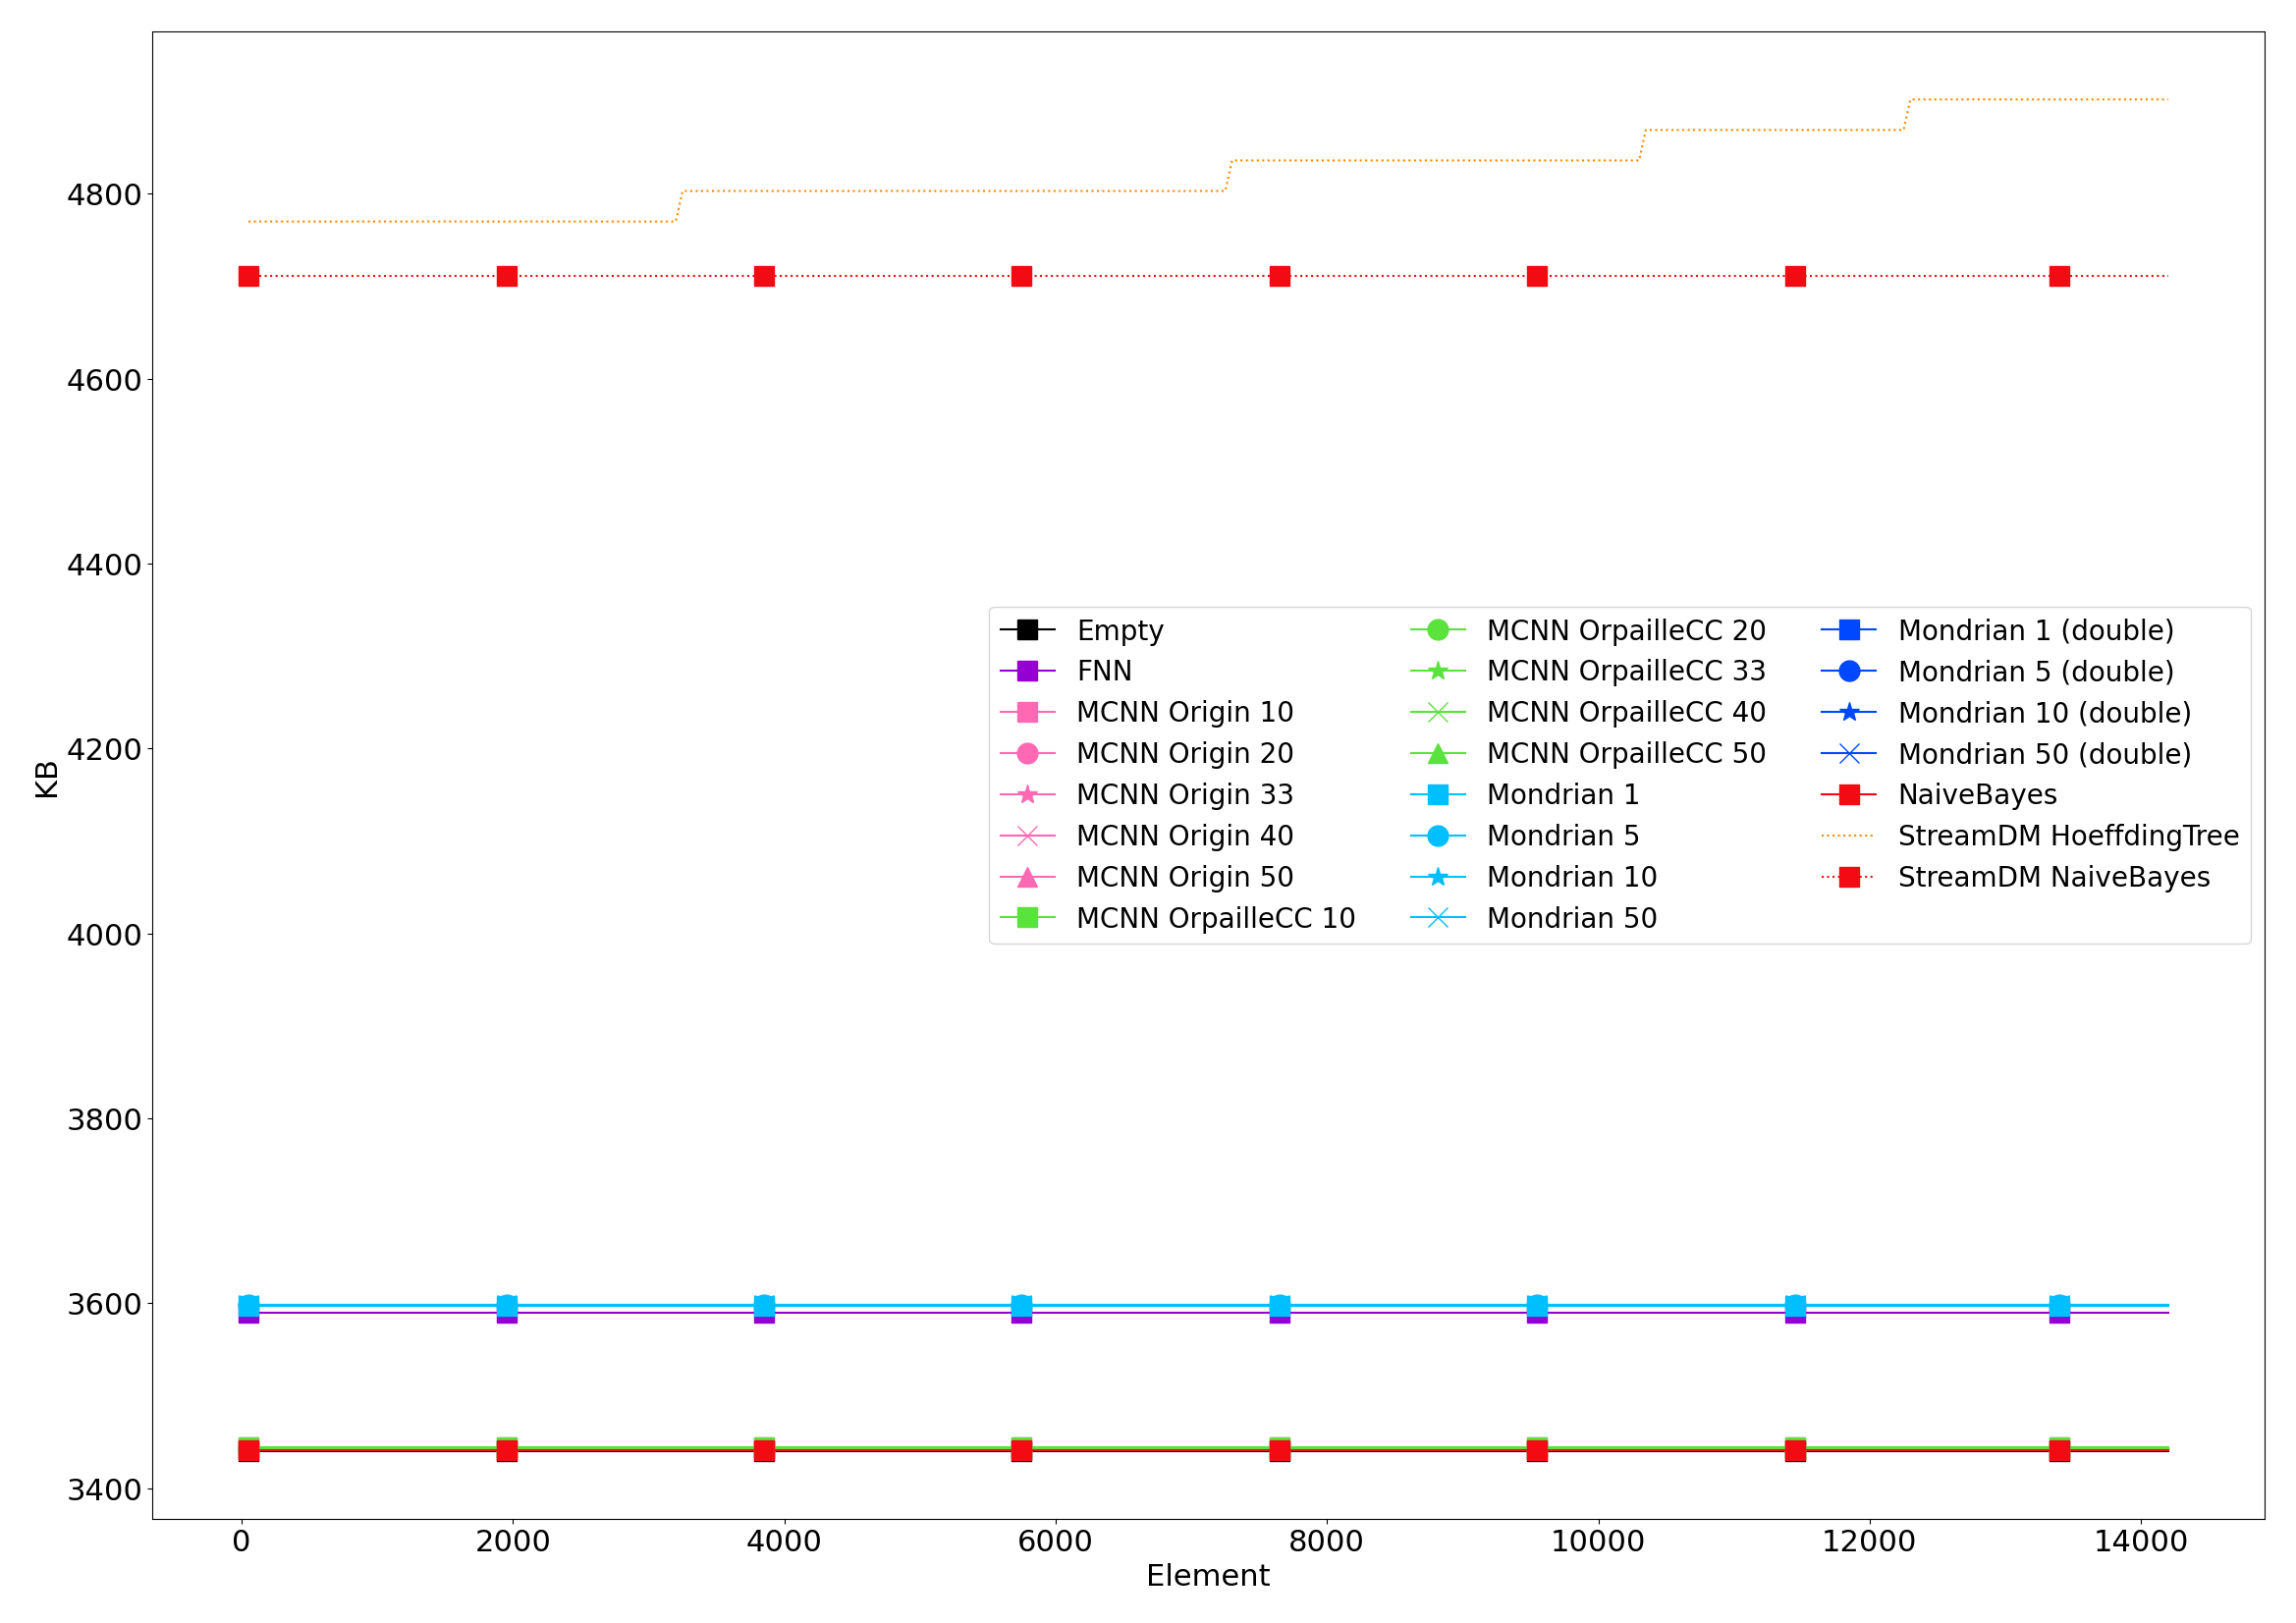
\includegraphics[width=\linewidth]{figures/results/banos_3_memory.png}
	\caption{Memory footprint of the classifiers relatively to the empty
	classifier, measured on the \banosdataset dataset. The memory footprint of the empty
	classifier is slightly above 3.439KB.}
	\label{fig:memory}
\end{figure}


\subsection{Micro-Cluster Nearest Neighbor Hyperparameters}

Figure~\ref{fig:mcnn-tuning-error} shows the impact of the error threshold
in the \mcnn classifiers with different cluster counts. The error
threshold of \mcnn has little impact on the classification performance. For
20 and 40 clusters, the best-performing threshold is either 2 or 4, meaning
that a cluster may do 2 or 4 errors before being split. For 10 clusters,
all error thresholds perform equally.

\begin{figure}
	 \begin{subfigure}[b]{0.49\textwidth}
		 \centering
		 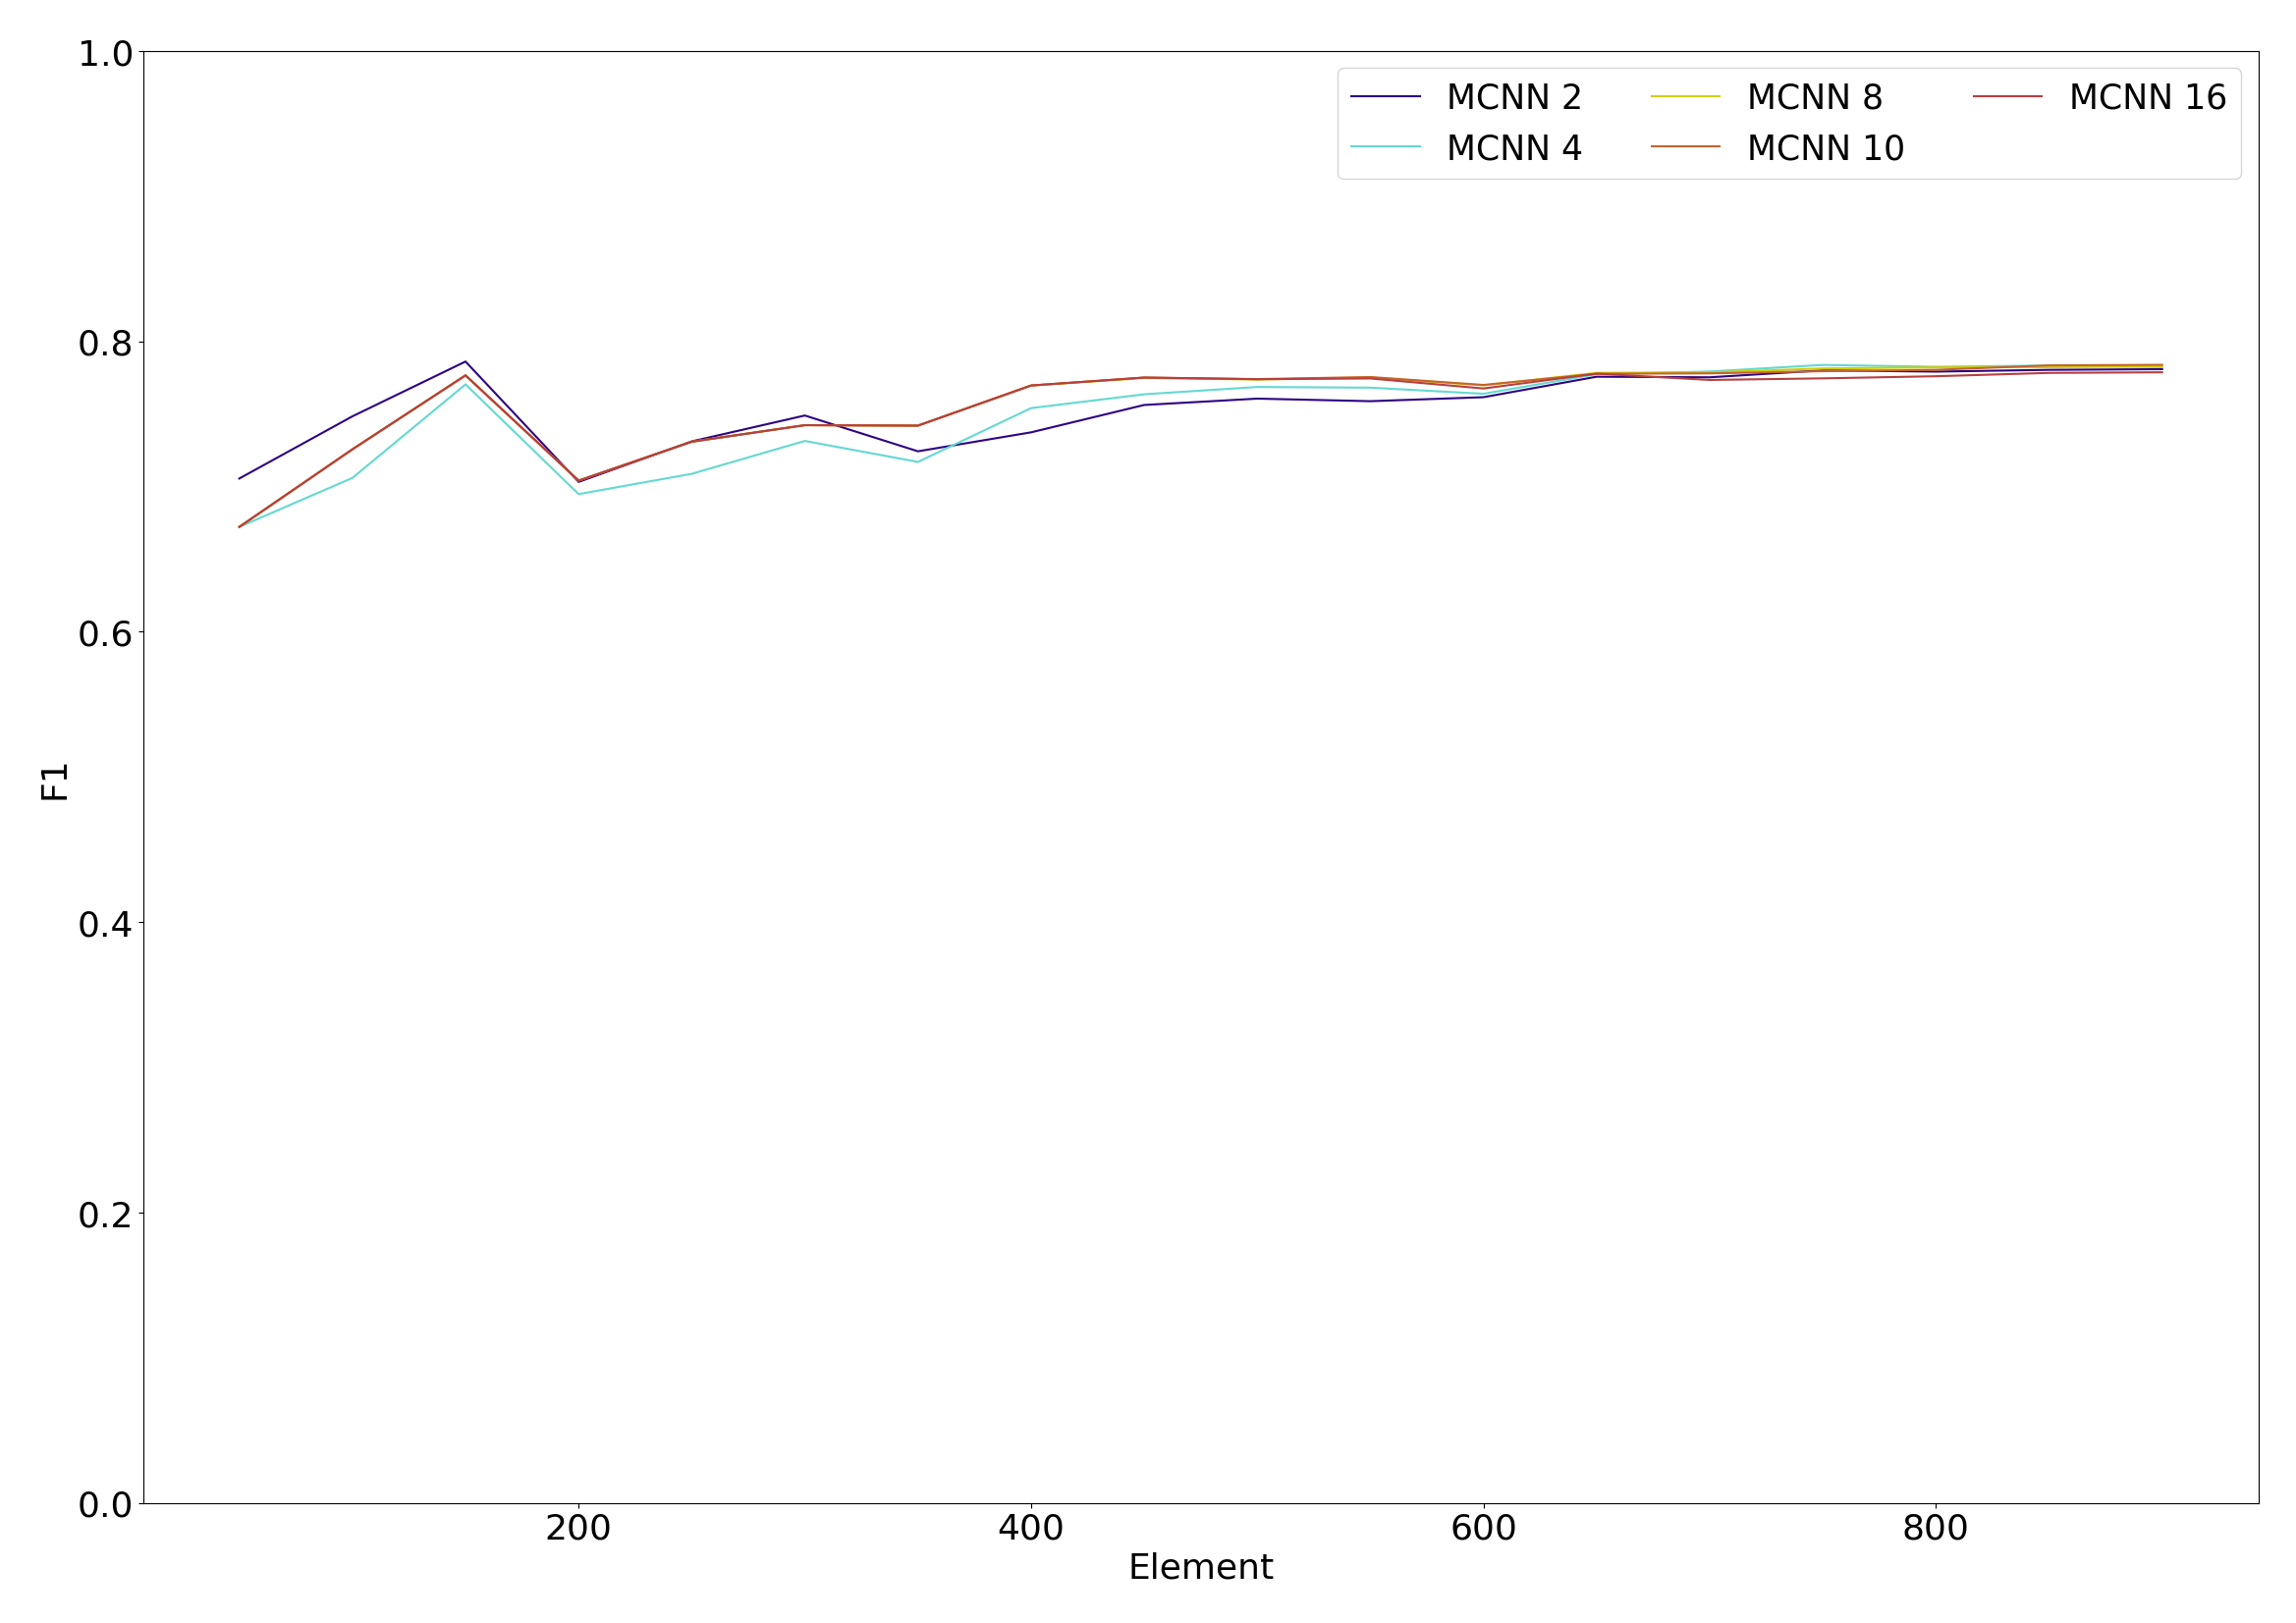
\includegraphics[width=\linewidth]{figures/calibration_mcnn_40.png}
		 \caption{40 clusters}
	 \end{subfigure}
	 \begin{subfigure}[b]{0.49\textwidth}
		 \centering
		 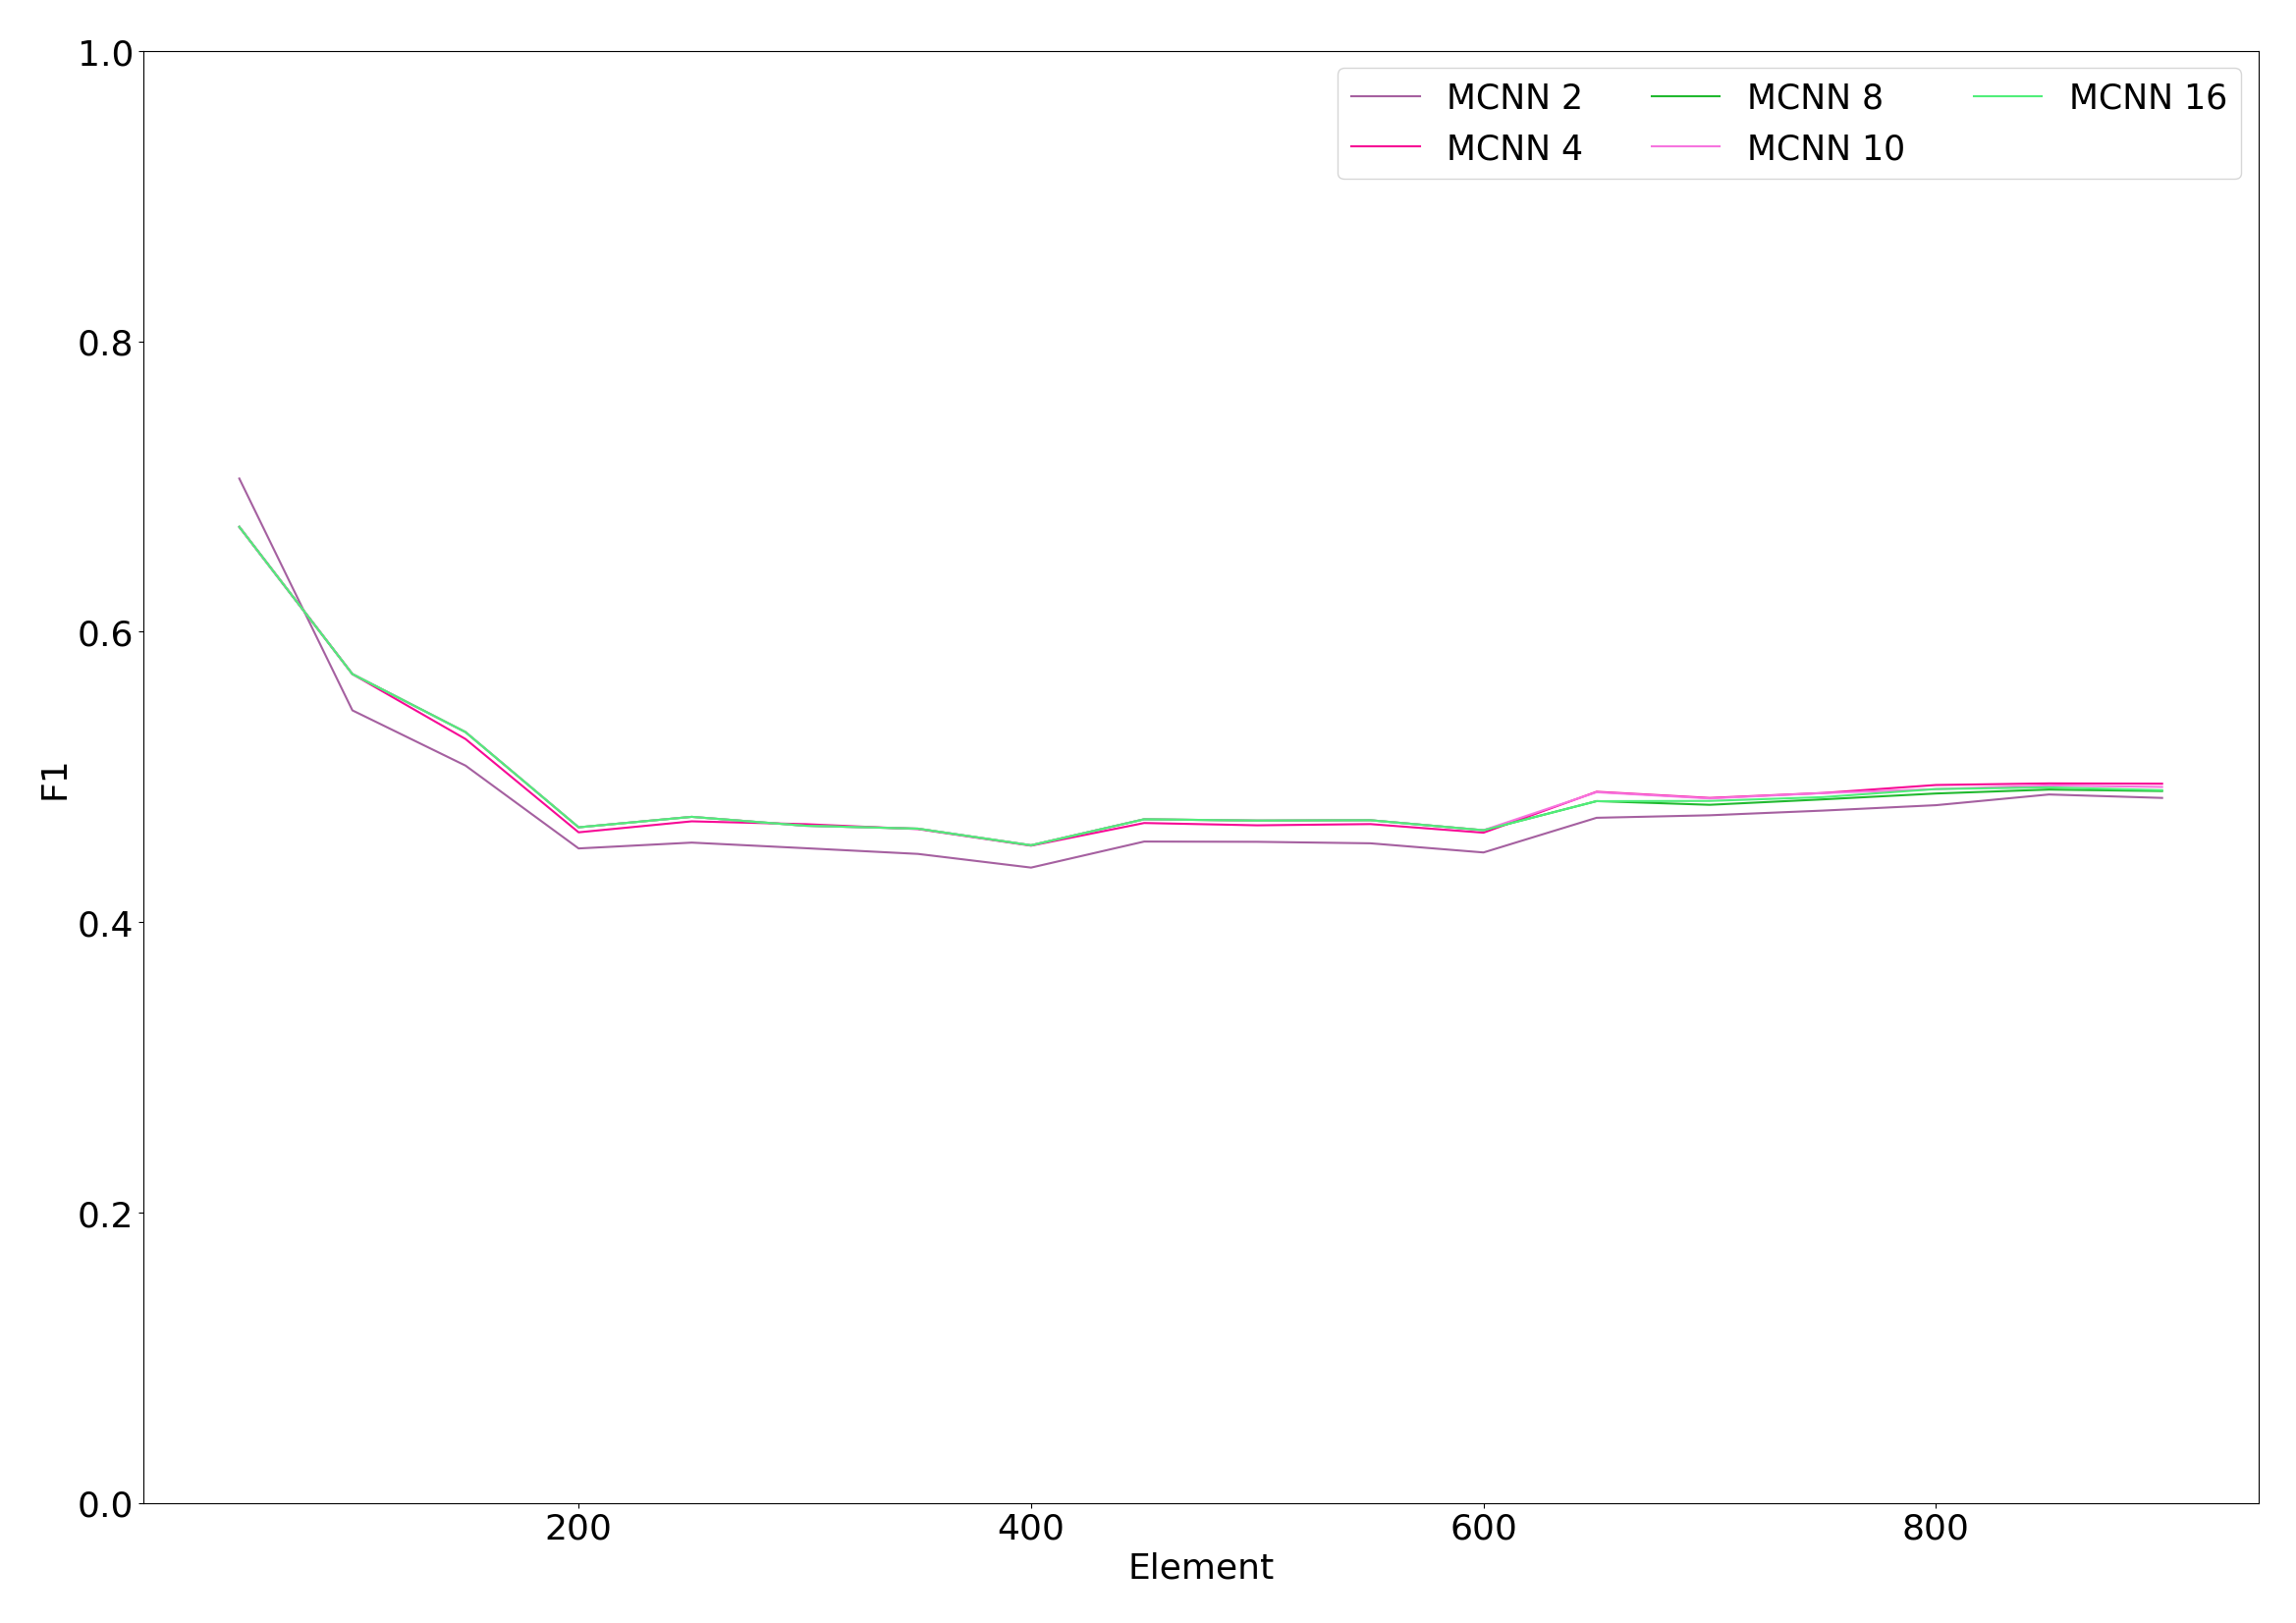
\includegraphics[width=\linewidth]{figures/calibration_mcnn_20.png}
		 \caption{20 clusters}
	 \end{subfigure}
	 \begin{subfigure}[b]{0.49\textwidth}
		 \centering
		 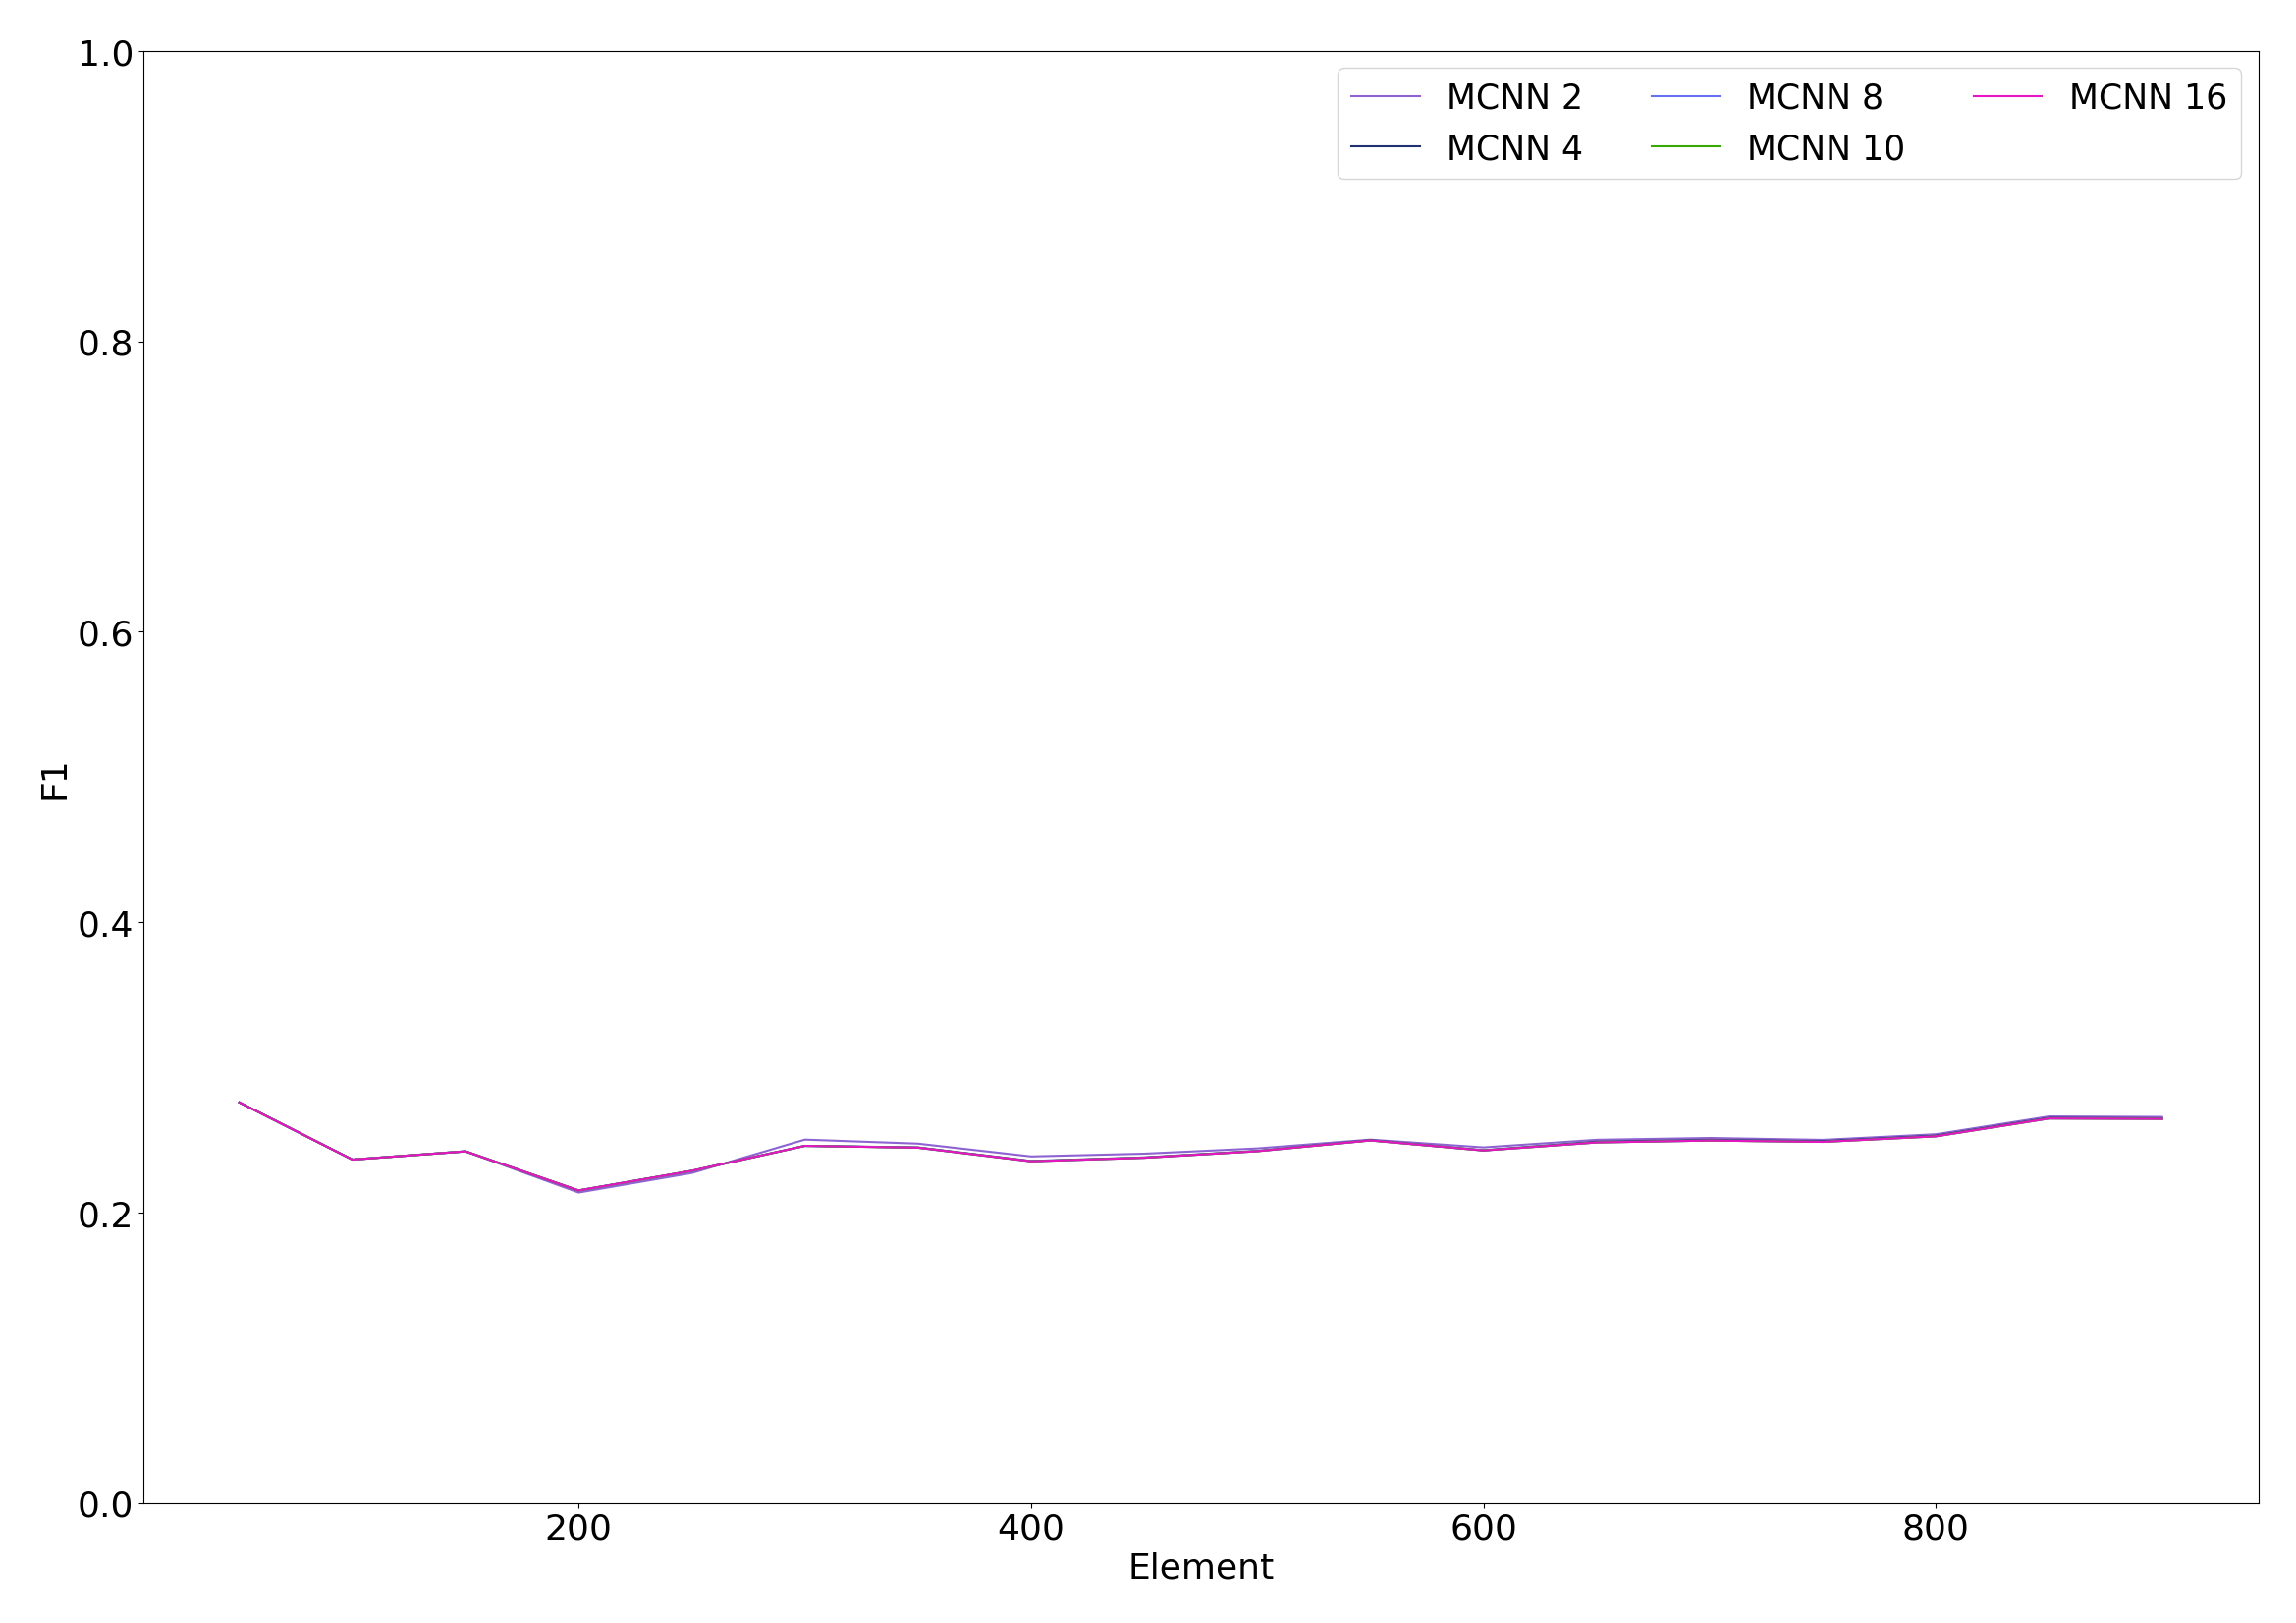
\includegraphics[width=\linewidth]{figures/calibration_mcnn_10.png}
		 \caption{10 clusters}
	 \end{subfigure}
	\caption{Error threshold tuning of \mcnn with first subject of \banosdataset dataset.}
	\label{fig:mcnn-tuning-error}
\end{figure}

\subsection{\mondrianforest Hyperparameters}

Figure~\ref{fig:mondrian-tuning} shows the impact of the \mondrianforest hyperparameters on
the classification performance. 

The base count hyperparameter (Figure~\ref{fig:mondrian-base-count}) has a
very substantial impact on classification performance; the smallest value
(0.0) results in the best performance. On the contrary, the
budget hyperparameter (Figure~\ref{fig:mondrian-budget}) only has a
moderate impact on classification; the best value is 0.2. Finally, the discount hyperparameter
(Figure~\ref{fig:mondrian-discount}) has a negligible impact on the
performance; the best-performing value is 0.1.

\begin{figure}
	 \centering
	 \begin{subfigure}[b]{0.49\textwidth}
		\centering
		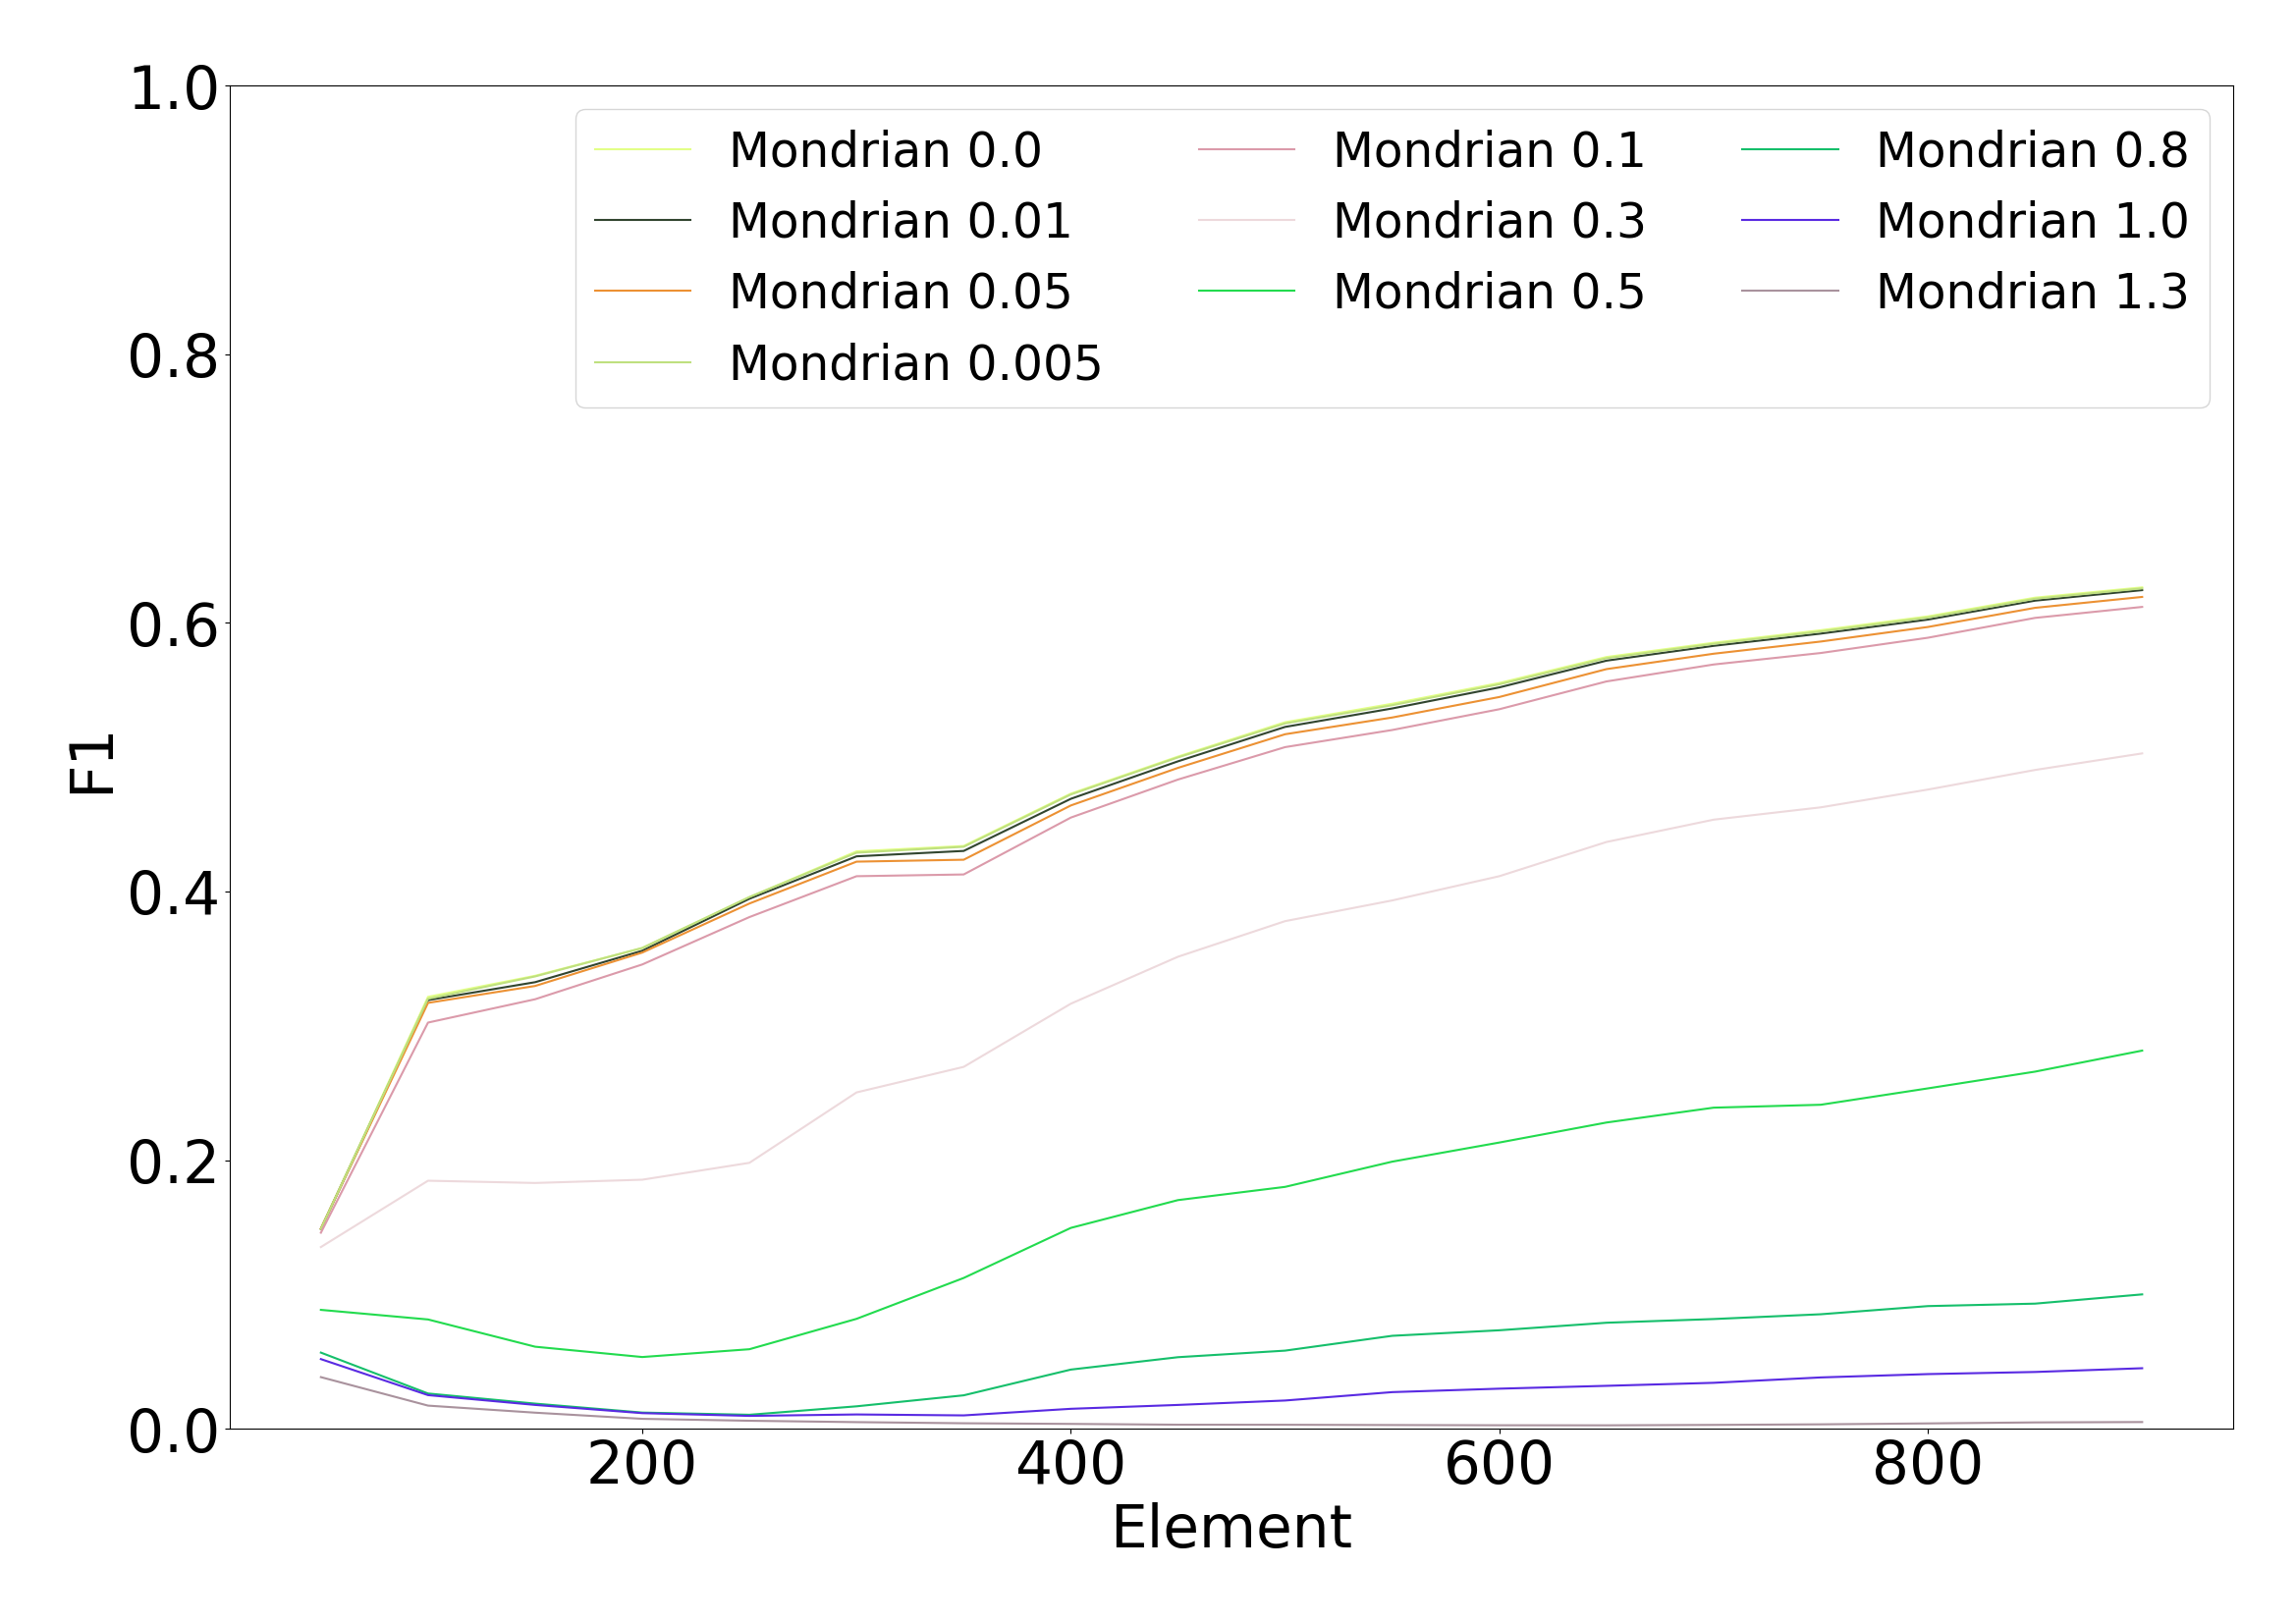
\includegraphics[width=\textwidth]{figures/calibration_mondrian_base.png}
		\caption{Impact of the base count with 10 trees, a budget of $1.0$, and a discount factor of $0.2$.} 
		\label{fig:mondrian-base-count}
	\end{subfigure}
	\hfill
	 \begin{subfigure}[b]{0.49\textwidth}
		 \centering
		 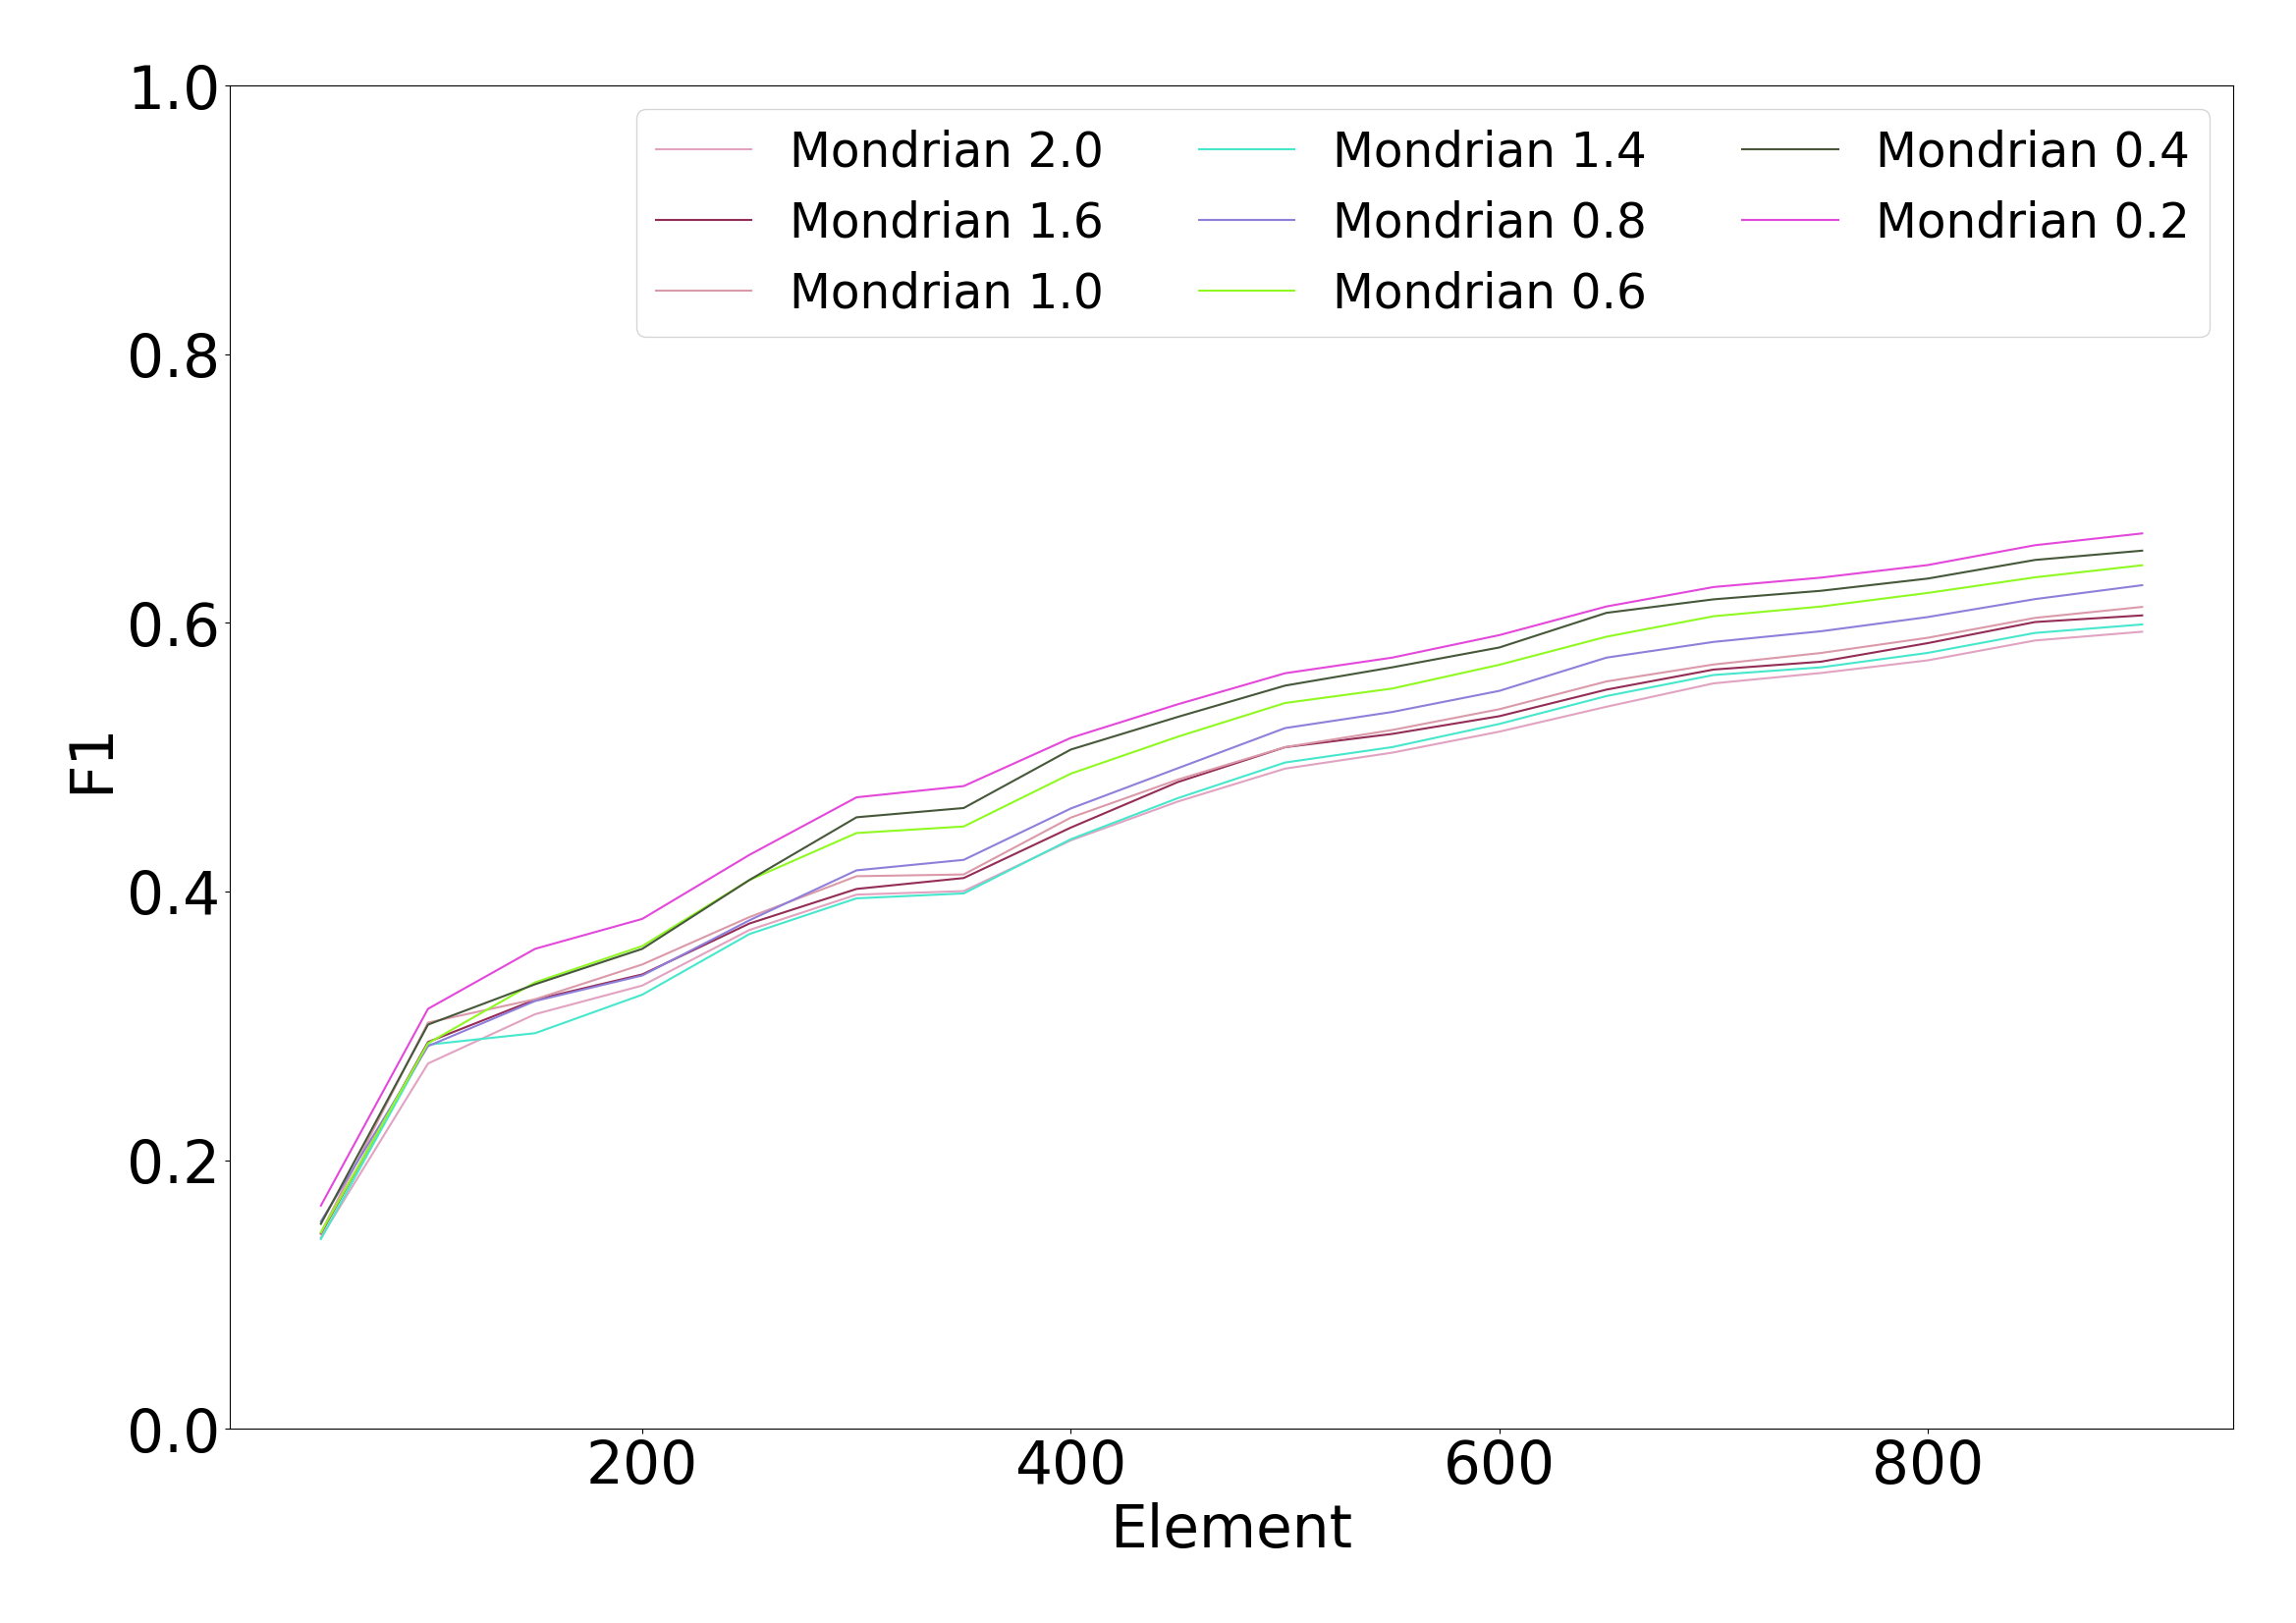
\includegraphics[width=\textwidth]{figures/calibration_mondrian_lifetime.png}
		 \caption{Impact of the budget with 10 trees, a base count of $0.1$, and discount factor of $0.2$.}
		 \label{fig:mondrian-budget}
	 \end{subfigure}
	 \hfill
	 \begin{subfigure}[b]{0.49\textwidth}
		 \centering
		 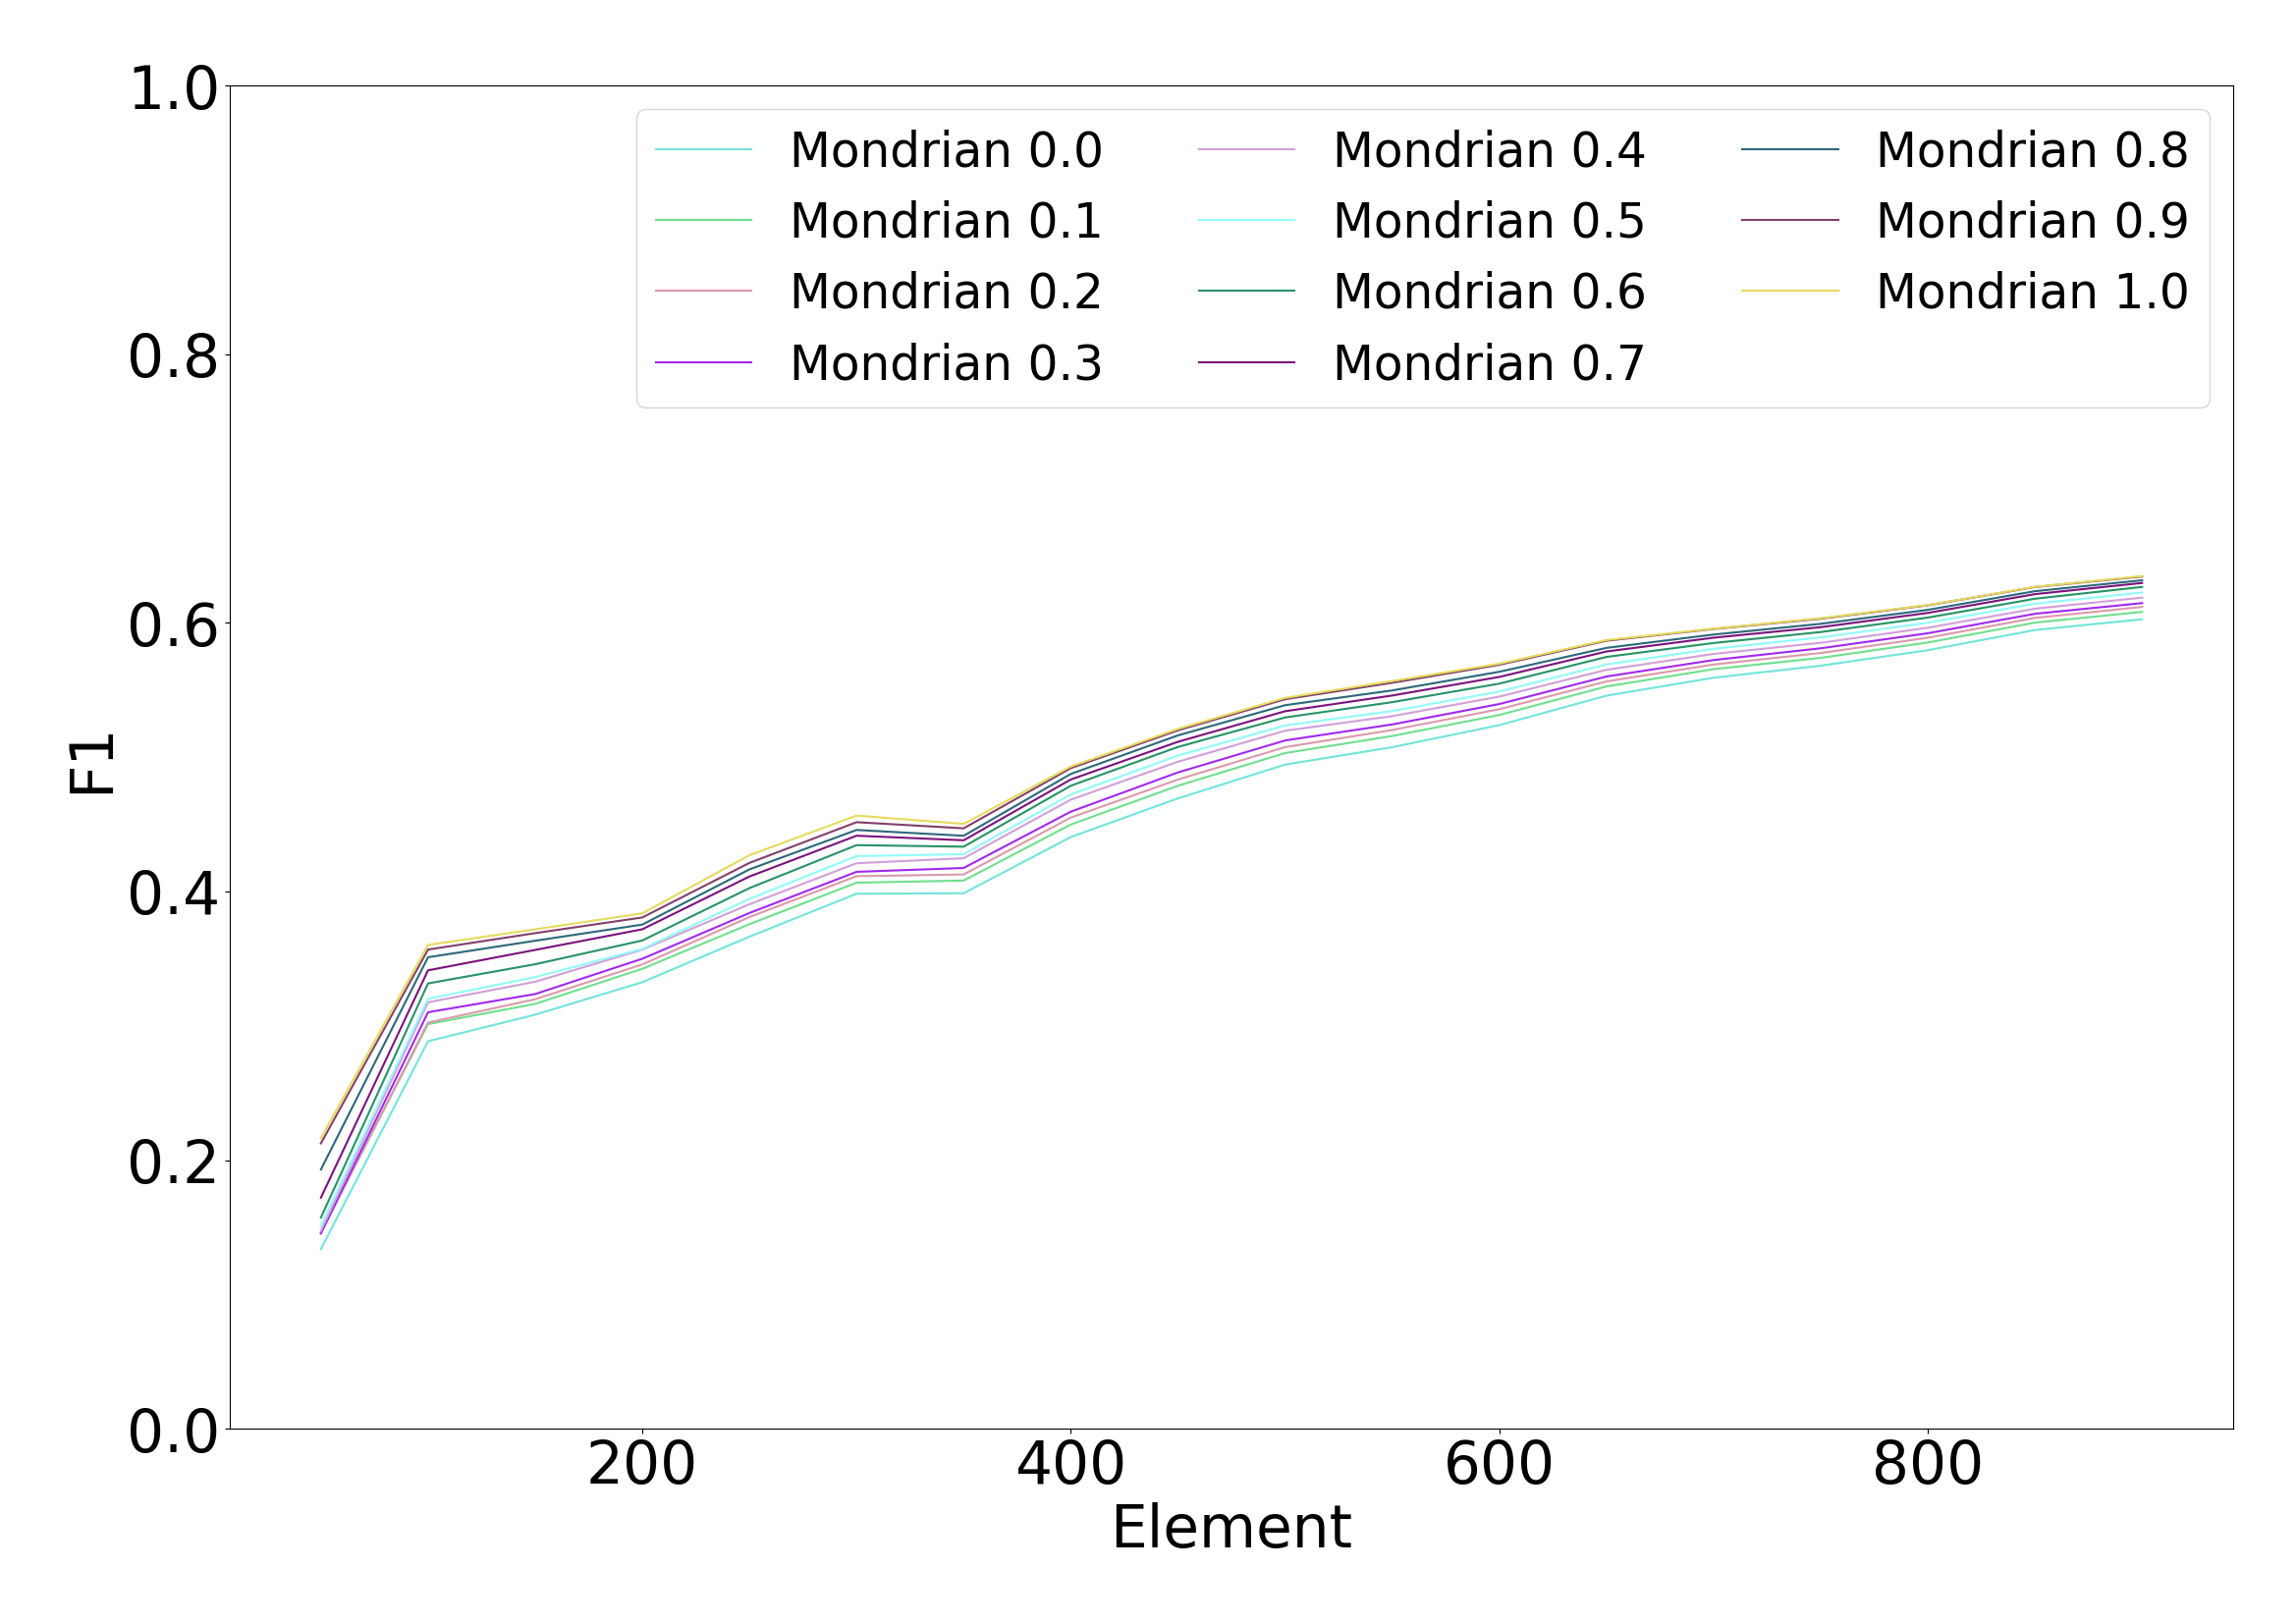
\includegraphics[width=\textwidth]{figures/calibration_mondrian_discount.png}
		 \caption{Impact of the discount factor with 10 trees, a budget of $1.0$, and a base count of $0.1$.}
		 \label{fig:mondrian-discount}
	 \end{subfigure}
		\caption{Hyperparameters tuning for Mondrian with first subject of \banosdataset dataset.}
		\label{fig:mondrian-tuning}
\end{figure}


